%% abtex2-modelo-trabalho-academico.tex, v-1.9.5 laurocesar
%% Copyright 2012-2015 by abnTeX2 group at http://www.abntex.net.br/ 
%%
%% This work may be distributed and/or modified under the
%% conditions of the LaTeX Project Public License, either version 1.3
%% of this license or (at your option) any later version.
%% The latest version of this license i\draw[red,fill=red] (3.5,-2.5) circle (2ex);s in
%%   http://www.latex-project.org/lppl.txt
%% and version 1.3 or later is part of all distributions of LaTeX
%% version 2005/12/01 or later.
%%
%% This work has the LPPL maintenance status `maintained'.
%% 
%% The Current Maintainer of this work is the abnTeX2 team, led
%% by Lauro César Araujo. Further information are available on 
%% http://www.abntex.net.br/
%%
%% This work consists of the files abntex2-modelo-trabalho-academico.tex,
%% abntex2-modelo-include-dissertationdissertationcomandos and abntex2-modelo-references.bib
%%

% ------------------------------------------------------------------------
% ------------------------------------------------------------------------
% abnTeX2: Modelo de Trabalho Academico (tese de doutorado, dissertacao de
% mestrado e trabalhos monograficos em geral) em conformidade com 
% ABNT NBR 14724:2011: Informacao e documentacao - Trabalhos academicos -
% Apresentacao
% ------------------------------------------------------------------------
% ------------------------------------------------------------------------

\documentclass[
	% -- opções da classe memoir --
	12pt,				% tamanho da fonte
	openright,		nsubseteq	% capítulos começam em pág ímpar (insere página vazia caso preciso)
	twoside,			% para impressão em verso e anverso. Oposto a oneside
	a4paper,			% tamanho do papel. 
	% -- opções da classe abntex2 --
	%chapter=TITLE,		% títulos de capítulos convertidos em letras maiúsculas
	%section=TITLE,		% títulos de seções convertidos em letras maiúsculas
	%subsection=TITLE,	% títulos de subseções convertidos em letras maiúsculas
	%subsubsection=TITLE,% títulos de subsubseções convertidos em letras maiúsculas
	% -- opções do pacote babel --
	english,			% idioma adicional para hifenização
	french,				% idioma adicional para hifenização
	spanish,			% idioma adicional para hifenização
	brazil				% o último idioma é o principal do documento
	]{abntex2}

% ---
% Pacotes básicos 
% ---
\usepackage{lmodern}			% Usa a fonte Latin Modern			
\usepackage[T1]{fontenc}		% Selecao de codigos de fonte.
\usepackage[utf8]{inputenc}		% Codificacao do documento (conversão automática dos acentos)
\usepackage{lastpage}			% Usado pela Ficha catalográfica
\usepackage{indentfirst}		% Indenta o primeiro parágrafo de cada seção.
\usepackage{color}				% Controle das cores
\usepackage{graphicx}			% Inclusão de gráficos
\usepackage{microtype} 			% para melhorias de justificação
% ---

\usepackage{longtable}	

\usepackage{multirow}

% ---
% Pacotes adicionais, usados apenas no âmbito do Modelo Canônico do abnteX2
% ---
\usepackage{lipsum}				% para geração de dummy text
% ---

% ---
% Pacotes de citações
% ---
\usepackage[english,hyperpageref]{backref}	 % Paginas com as citações na bibl
\usepackage[alf]{abntex2cite}	% Citações padrão ABNT

%for formula references
\usepackage{amsmath}

% Pacotes %triangledown
\usepackage{latexsym}
\usepackage{amssymb}
\usepackage{amsfonts}
\usepackage{amsthm}

\usepackage[linesnumbered,ruled,vlined]{algorithm2e}

%langle
\usepackage{scalerel}

%draw 8 tile puzzle
\usepackage{forest}
\usetikzlibrary[calc]

% to shrink figures
\usepackage{tikz-qtree}

% for letters
\usepackage{mathcomp}
\DeclareMathAlphabet{\mathpzc}{OT1}{pzc}{m}{it}


% draw lines
\usepackage{tikz}
\usetikzlibrary{arrows}
\usetikzlibrary{decorations.pathreplacing} 

% -- square with colors
\usepackage{xcolor}

% -- crossover
\usepackage{xr}

% work with columns of table
\usepackage{array}

% cartesian plane
%\usepackage{tkz-euclide}
\usepackage{tikz}
\usepackage{verbatim}

% symbols
\usepackage{pifont}

\providecommand{\shortcite}[1]{\cite{#1}}

% to draw thing horizontally
\usepackage{lscape}

% Theorems
\newtheorem{theorem}{Theorem}[section]
\newtheorem{corollary}{Corollary}[theorem]
\newtheorem{lemma}[theorem]{Lemma}
\newtheorem{definition}{Definition}[section]
% --- 
% CONFIGURAÇÕES DE PACOTES
% --- 

% limits underneath
\DeclareMathOperator*{\argminA}{arg\,min} % Jan Hlavacek
\DeclareMathOperator*{\argminB}{argmin}   % Jan Hlavacek
\DeclareMathOperator*{\argminC}{\arg\min}   % rbp

  % impressao do nome do capitulo - part
  \renewcommand{\printpartname}{%
   \chaptitlefont
   {Chapter}%
  }

\addto\captionsenglish{
	\renewcommand{\orientadorname}{Orientador:}
	\renewcommand{\coorientadorname}{Co-orientador:}
}
% ---
% Configurações do pacote backref
% Usado sem a opção hyperpageref de backref
\renewcommand{\backrefpagesname}{Citado na(s) página(s):~}
% Texto padrão antes do número das páginas
\renewcommand{\backref}{}
% Define os textos da citação
\renewcommand*{\backrefalt}[4]{
	\ifcase #1 %
		Nenhuma citação no texto.%
	\or
		Citado na página #2.%
	\else
		Citado #1 vezes nas páginas #2.%
	\fi}%
% ---

% -- Square with colors

\newcommand\crule[3][white]{\textcolor{#1}{\rule{#2}{#3}}}
\newcommand\sanit[3][white]{\color{#1}{\rule{#2}{#3}}}

% ---
% Configuracao de forest
%draw 8 tile puzzle
\newcommand{\ninepuzzle}[1]{%
\begin{tikzpicture}
    \foreach [count=\i] \val in {#1} { 
        \draw[fill=white, draw=black]  let \n{row}={int(mod(\i -1, 3))}, \n{col}={ int( ( \i - 1 ) / (-3) ) } in 
            (\n{row}, \n{col}) rectangle  +(1,1) 
            +(0.5, 0.5) node{\val};
            %\filldraw[fill=green, draw=blue];
    }
\end{tikzpicture}%    
}

%draw small 8 tile puzzle for DFS
\newcommand{\ninepuzzlesmall}[2]{%
\begin{tikzpicture}[scale = 0.4]
	\draw [decorate,xshift=4pt,yshift=28pt] node [black,midway,yshift=0.5cm] 
{\footnotesize \huge{#2}};
    \foreach [count=\i] \val in {#1} {
        \draw[fill=white, draw=black]  let \n{row}={int(mod(\i -1, 3))}, \n{col}={ int( ( \i - 1 ) / (-3) ) } in 
            (\n{row}, \n{col}) rectangle  +(1,1) 
            +(0.5, 0.5) node{\val};
            %\filldraw[fill=green, draw=blue];
    }
\end{tikzpicture}%    
}

%draw small 8 tile puzzle for BFS
\newcommand{\ninepuzzlesmallbfs}[2]{%
\begin{tikzpicture}[scale = 0.4]
	\draw [decorate,xshift=4pt,yshift=28pt] node [black,midway,yshift=0.5cm] 
{\footnotesize \huge{#2}};
    \foreach [count=\i] \val in {#1} {
        \draw[fill=white, draw=black]  let \n{row}={int(mod(\i -1, 3))}, \n{col}={ int( ( \i - 1 ) / (-3) ) } in 
            (\n{row}, \n{col}) rectangle  +(1,1) 
            +(0.5, 0.5) node{\val};
            %\filldraw[fill=green, draw=blue];
    }
\end{tikzpicture}%    
}

\newcommand{\ninepuzzlets}[1]{%
\begin{tikzpicture}
    \foreach [count=\i] \val/\colone in {#1} { 
        \draw[fill=\colone, draw=black]  let \n{row}={int(mod(\i -1, 3))}, \n{col}={ int( ( \i - 1 ) / (-3) ) } in 
            (\n{row}, \n{col}) rectangle  +(1,1) 
            +(0.5, 0.5) node{\val};
            %\filldraw[fill=green, draw=blue];
    }
\end{tikzpicture}%    
}

% --block worlds
\newcommand{\blockworlds}[1]{%
\begin{tikzpicture}
    \foreach [count=\i] \val/\colone in {#1} { 
        \draw[fill=\colone, draw=black]  let \n{row}={int(mod(\i -1, 3))}, \n{col}={ int( ( \i - 1 ) / (-3) ) } in 
            (\n{row}, \n{col}) rectangle  +(2,2) 
            +(0.5, 0.5) node[font=\large\bfseries,text width=-1em, color=black]{\huge \val};
    }
\end{tikzpicture}%    
}
% --end block worlds

% --block worlds
\newcommand{\blockworldsunordered}[1]{%
\begin{tikzpicture}
    \foreach [count=\i] \val/\colone in {#1} { 
        \draw[fill=\colone, draw=black]  let \n{row}={int(mod(2*\i , 1))}, \n{col}={ int( ( 2*\i  ) / (-1) ) } in 
            (\n{row}, \n{col}) rectangle  +(2,2) 
            +(0.5, 0.5) node[font=\large\bfseries,text width=-1em, color=black]{\huge \val};
    }
\end{tikzpicture}%    
}
% --end block worlds
\newsavebox\myboxa
\newsavebox\myboxb
\newsavebox\myboxc

% begin DFS

\newsavebox\myboxone
\newsavebox\myboxtwo
\newsavebox\myboxthree
\newsavebox\myboxfour
\newsavebox\myboxfive
\newsavebox\myboxsix
\newsavebox\myboxseven
\newsavebox\myboxeight
\newsavebox\myboxnine
\newsavebox\myboxten
\newsavebox\myboxeleven
\newsavebox\myboxtwelve
\newsavebox\myboxthirteen
\newsavebox\myboxfourteen
\newsavebox\myboxfifteen
\newsavebox\myboxsixteen
\newsavebox\myboxseventeen
\newsavebox\myboxeighteen
\newsavebox\myboxnineteen
\newsavebox\myboxtwenty
\newsavebox\myboxtwentyone
\newsavebox\myboxtwentytwo
\newsavebox\myboxtwentythree
\newsavebox\myboxtwentyfour
\newsavebox\myboxtwentyfive
\newsavebox\myboxtwentysix
\newsavebox\myboxtwentyseven
\newsavebox\myboxtwentyeight
\newsavebox\myboxtwentynine
\newsavebox\myboxthirty
\newsavebox\myboxthirtyone

\savebox\myboxone{\ninepuzzlesmall{2,8,3,1,6,4,7, ,5}{1}}
\savebox\myboxtwo{\ninepuzzlesmall{2,8,3,1,6,4, ,7,5}{2}}
\savebox\myboxthree{\ninepuzzlesmall{2,8,3, ,6,4,1,7,5}{3}}
\savebox\myboxfour{\ninepuzzlesmall{ ,8,3,2,6,4,1,7,5}{4}}
\savebox\myboxfive{\ninepuzzlesmall{8, ,3,2,6,4,1,7,5}{5}}
\savebox\myboxsix{\ninepuzzlesmall{8,3, ,2,6,4,1,7,5}{6}}
\savebox\myboxseven{\ninepuzzlesmall{8,6,3,2, ,4,1,7,5}{7}}
\savebox\myboxeight{\ninepuzzlesmall{2,8,3,6, ,4,1,7,5}{8}}
\savebox\myboxnine{\ninepuzzlesmall{2, ,3,6,8,4,1,7,5}{9}}
\savebox\myboxten{\ninepuzzlesmall{ ,2,3,6,8,4,1,7,5}{10}}
\savebox\myboxeleven{\ninepuzzlesmall{2,3, ,6,8,4,1,7,5}{11}}
\savebox\myboxtwelve{\ninepuzzlesmall{2,8,3,6,4, ,1,7,5}{12}}
\savebox\myboxthirteen{\ninepuzzlesmall{2,8, ,6,4,3,1,7,5}{13}}
\savebox\myboxfourteen{\ninepuzzlesmall{2,8,3,6,4,5,1,7, }{14}}
\savebox\myboxfifteen{\ninepuzzlesmall{2,8,3,6,7,4,1, ,5}{15}}
\savebox\myboxsixteen{\ninepuzzlesmall{2,8,3,6,7,4, ,1,5}{16}}
\savebox\myboxseventeen{\ninepuzzlesmall{2,8,3,6,7,4,1,5, }{17}}
\savebox\myboxeighteen{\ninepuzzlesmall{2,8,3,1, ,4,7,6,5}{18}}
\savebox\myboxnineteen{\ninepuzzlesmall{2,8,3, ,1,4,7,6,5}{19}}
\savebox\myboxtwenty{\ninepuzzlesmall{ ,8,3,2,1,4,7,6,5}{20}}
\savebox\myboxtwentyone{\ninepuzzlesmall{8, ,3,2,1,4,7,6,5}{21}}
\savebox\myboxtwentytwo{\ninepuzzlesmall{8,3, ,2,1,4,7,6,5}{22}}
\savebox\myboxtwentythree{\ninepuzzlesmall{8,1,3,2, ,4,7,6,5}{23}}
\savebox\myboxtwentyfour{\ninepuzzlesmall{2,8,3,7,1,4, ,6,5}{24}}
\savebox\myboxtwentyfive{\ninepuzzlesmall{2,8,3,7,1,4,6, ,5}{25}}
\savebox\myboxtwentysix{\ninepuzzlesmall{2,8,3,7, ,4,6,1,5}{26}}
\savebox\myboxtwentyseven{\ninepuzzlesmall{2,8,3,7,1,4,6,5, }{27}}
\savebox\myboxtwentyeight{\ninepuzzlesmall{2, ,3,1,8,4,7,6,5}{28}}
\savebox\myboxtwentynine{\ninepuzzlesmall{ ,2,3,1,8,4,7,6,5}{29}}
\savebox\myboxthirty{\ninepuzzlesmall{1,2,3, ,8,4,7,6,5}{30}}
\savebox\myboxthirtyone{\ninepuzzlesmall{1,2,3,8, ,4,7,6,5}{31}}

% end DFS

% begin BFS

\newsavebox\myboxbfsone
\newsavebox\myboxbfstwo
\newsavebox\myboxbfsthree
\newsavebox\myboxbfsfour
\newsavebox\myboxbfsfive
\newsavebox\myboxbfssix
\newsavebox\myboxbfsseven
\newsavebox\myboxbfseight
\newsavebox\myboxbfsnine
\newsavebox\myboxbfsten
\newsavebox\myboxbfseleven
\newsavebox\myboxbfstwelve
\newsavebox\myboxbfsthirteen
\newsavebox\myboxbfsfourteen
\newsavebox\myboxbfsfifteen
\newsavebox\myboxbfssixteen
\newsavebox\myboxbfsseventeen
\newsavebox\myboxbfseighteen
\newsavebox\myboxbfsnineteen
\newsavebox\myboxbfstwenty
\newsavebox\myboxbfstwentyone
\newsavebox\myboxbfstwentytwo
\newsavebox\myboxbfstwentythree
\newsavebox\myboxbfstwentyfour
\newsavebox\myboxbfstwentyfive
\newsavebox\myboxbfstwentysix
\newsavebox\myboxbfstwentyseven
\newsavebox\myboxbfstwentyeight
\newsavebox\myboxbfstwentynine
\newsavebox\myboxbfsthirty
\newsavebox\myboxbfsthirtyone
\newsavebox\myboxbfsthirtytwo
\newsavebox\myboxbfsthirtythree
\newsavebox\myboxbfsthirtyfour
\newsavebox\myboxbfsthirtyfive
\newsavebox\myboxbfsthirtysix
\newsavebox\myboxbfsthirtyseven
\newsavebox\myboxbfsthirtyeight
\newsavebox\myboxbfsthirtynine
\newsavebox\myboxbfsforty
\newsavebox\myboxbfsfortyone
\newsavebox\myboxbfsfortytwo
\newsavebox\myboxbfsfortythree
\newsavebox\myboxbfsfortyfour
\newsavebox\myboxbfsfortyfive
\newsavebox\myboxbfsfortysix


\savebox\myboxbfsone{\ninepuzzlesmallbfs{2,8,3,1,6,4,7, ,5}{1}}
\savebox\myboxbfstwo{\ninepuzzlesmallbfs{2,8,3,1,6,4, ,7,5}{2}}
\savebox\myboxbfsthree{\ninepuzzlesmallbfs{2,8,3,1, ,4,7,6,5}{3}}
\savebox\myboxbfsfour{\ninepuzzlesmallbfs{2,8,3,1,6,4,7,5, }{4}}
\savebox\myboxbfsfive{\ninepuzzlesmallbfs{2,8,3, ,6,4,1,7,5}{5}}
\savebox\myboxbfssix{\ninepuzzlesmallbfs{2,8,3, ,1,4,7,6,5}{6}}
\savebox\myboxbfsseven{\ninepuzzlesmallbfs{2, ,3,1,8,4,7,6,5}{7}}
\savebox\myboxbfseight{\ninepuzzlesmallbfs{2,8,3,1,4, ,7,6,5}{8}}
\savebox\myboxbfsnine{\ninepuzzlesmallbfs{2,8,3,1,6, ,7,5,4}{9}}
\savebox\myboxbfsten{\ninepuzzlesmallbfs{ ,8,3,2,6,4,1,7,5}{10}}
\savebox\myboxbfseleven{\ninepuzzlesmallbfs{2,8,3,6, ,4,1,7,5}{11}}
\savebox\myboxbfstwelve{\ninepuzzlesmallbfs{ ,8,3,2,1,4,7,6,5}{12}}
\savebox\myboxbfsthirteen{\ninepuzzlesmallbfs{2,8,3,7,1,4, ,6,5}{13}}
\savebox\myboxbfsfourteen{\ninepuzzlesmallbfs{ ,2,3,1,8,4,7,6,5}{14}}
\savebox\myboxbfsfifteen{\ninepuzzlesmallbfs{2,3, ,1,8,4,7,6,5}{15}}
\savebox\myboxbfssixteen{\ninepuzzlesmallbfs{2,8, ,1,4,3,7,6,5}{16}}
\savebox\myboxbfsseventeen{\ninepuzzlesmallbfs{2,8,3,1,4,5,7,6, }{17}}
\savebox\myboxbfseighteen{\ninepuzzlesmallbfs{2,8,3,1, ,6,7,5,4}{18}}
\savebox\myboxbfsnineteen{\ninepuzzlesmallbfs{2,8, ,1,6,3,7,5,4}{19}}
\savebox\myboxbfstwenty{\ninepuzzlesmallbfs{8, ,3,2,6,4,1,7,5}{20}}
\savebox\myboxbfstwentyone{\ninepuzzlesmallbfs{2, ,3,6,8,4,1,7,5}{21}}
\savebox\myboxbfstwentytwo{\ninepuzzlesmallbfs{2,8,3,6,4, ,1,7,5}{22}}
\savebox\myboxbfstwentythree{\ninepuzzlesmallbfs{2,8,3,6,7,4,1, ,5}{23}}
\savebox\myboxbfstwentyfour{\ninepuzzlesmallbfs{8, ,3,2,1,4,7,6,5}{24}}
\savebox\myboxbfstwentyfive{\ninepuzzlesmallbfs{2,8,3,7,1,4,6, ,5}{25}}
\savebox\myboxbfstwentysix{\ninepuzzlesmallbfs{1,2,3, ,8,4,7,6,5}{26}}
\savebox\myboxbfstwentyseven{\ninepuzzlesmallbfs{2,3,4,1,8, ,7,6,5}{27}}
\savebox\myboxbfstwentyeight{\ninepuzzlesmallbfs{2, ,8,1,4,3,7,6,5}{28}}
\savebox\myboxbfstwentynine{\ninepuzzlesmallbfs{2,8,3,1,4,5,7, ,6}{29}}
\savebox\myboxbfsthirty{\ninepuzzlesmallbfs{2,8,3, ,1,6,7,5,4}{30}}
\savebox\myboxbfsthirtyone{\ninepuzzlesmallbfs{2, ,3,1,8,6,7,5,4}{31}}
\savebox\myboxbfsthirtytwo{\ninepuzzlesmallbfs{2,8,3,1,5,6,7, ,4}{32}}
\savebox\myboxbfsthirtythree{\ninepuzzlesmallbfs{2, ,8,1,6,3,7,5,4}{33}}
\savebox\myboxbfsthirtyfour{\ninepuzzlesmallbfs{8,3, ,2,6,4,1,7,5}{34}}
\savebox\myboxbfsthirtyfive{\ninepuzzlesmallbfs{8,6,3,2, ,4,1,7,5}{35}}
\savebox\myboxbfsthirtysix{\ninepuzzlesmallbfs{ ,2,3,6,8,4,1,7,5}{36}}
\savebox\myboxbfsthirtyseven{\ninepuzzlesmallbfs{2,3, ,6,8,4,1,7,5}{37}}
\savebox\myboxbfsthirtyeight{\ninepuzzlesmallbfs{2,8, ,6,4,3,1,7,5}{38}}
\savebox\myboxbfsthirtynine{\ninepuzzlesmallbfs{2,8,3,6,4,5,1,7, }{39}}
\savebox\myboxbfsforty{\ninepuzzlesmallbfs{2,8,3,6,7,4, ,1,5}{40}}
\savebox\myboxbfsfortyone{\ninepuzzlesmallbfs{2,8,3,6,7,4,1,5, }{41}}
\savebox\myboxbfsfortytwo{\ninepuzzlesmallbfs{8,3, ,2,1,4,7,6,5}{42}}
\savebox\myboxbfsfortythree{\ninepuzzlesmallbfs{8,1,3,2, ,4,7,6,5}{43}}
\savebox\myboxbfsfortyfour{\ninepuzzlesmallbfs{2,8,3,7, ,4,6,1,5}{44}}
\savebox\myboxbfsfortyfive{\ninepuzzlesmallbfs{2,8,3,7,1,4,6,5, }{45}}
\savebox\myboxbfsfortysix{\ninepuzzlesmallbfs{1,2,3,8, ,4,7,6,5}{46}}
% end BFS

\newsavebox\myboxcenter
\newsavebox\myboxcornerone
\newsavebox\myboxcornertwo
\newsavebox\myboxcornerthree
\newsavebox\myboxcornerfour
\newsavebox\myboxmediumleft
\newsavebox\myboxmediumup
\newsavebox\myboxmediumright
\newsavebox\myboxmediumdown

% -- block worlds
\newsavebox\myboxblockgreenone
\newsavebox\myboxblockbluetwo
\newsavebox\myboxblockredthree

\newsavebox\myboxblockteststar
\newsavebox\myboxblocktestend
% -- end block worlds

\savebox\myboxa{\ninepuzzle{4,1,2,8, ,3,5,7,6}}
\savebox\myboxb{\ninepuzzle{1,2,3,4,5,6,7,8, }}
\savebox\myboxc{\ninepuzzlets{C/cyan,E/yellow,C/cyan,E/yellow,M/white,E/yellow,C/cyan,E/yellow,C/cyan}}
% -- center
\savebox\myboxcenter{\ninepuzzlets{/red,/red,/red,/red,/white,/red,/red,/red,/red}}

% --corner left up = one

\savebox\myboxcornerone{\ninepuzzlets{/white,/red,/red,/red,/red,/red,/red,/red,/red}}

% -- medium left and medium up

\savebox\myboxmediumleft{\ninepuzzlets{/red,/red,/red,/white,/red,/red,/red,/red,/red}}
\savebox\myboxmediumup{\ninepuzzlets{/red,/white,/red,/red,/red,/red,/red,/red,/red}}

% -- corner three and corner two
\savebox\myboxcornerthree{\ninepuzzlets{/red,/red,/red,/red,/red,/red,/white,/red,/red}}
\savebox\myboxcornertwo{\ninepuzzlets{/red,/red,/white,/red,/red,/red,/red,/red,/red}}

% -- medium right and medium down

\savebox\myboxmediumdown{\ninepuzzlets{/red,/red,/red,/red,/red,/red,/red,/white,/red}}
\savebox\myboxmediumright{\ninepuzzlets{/red,/red,/red,/red,/red,/white,/red,/red,/red}}

% -- corner four

\savebox\myboxcornerfour{\ninepuzzlets{/red,/red,/red,/red,/red,/red,/red,/red,/white}}

% end type system

% -- block worlds
\savebox\myboxblockgreenone{\blockworlds{1/green}}
\savebox\myboxblockbluetwo{\blockworlds{2/blue}}
\savebox\myboxblockredthree{\blockworlds{3/red}}

\savebox\myboxblockteststar{\blockworldsunordered{1/green,2/blue}}
\savebox\myboxblocktestend{\blockworldsunordered{3/red,2/blue,1/green}}
% -- end block worlds


% -- draw eclipse
\newcommand{\boundellipse}[3]% center, xdim, ydim
{(#1) ellipse (#2 and #3)
}

% -- draw lines
\def\checkmark{\tikz\fill[scale=0.4](0,.35) -- (.25,0) -- (1,.7) -- (.25,.15) -- cycle;}
\tikzset{
  every point/.style = {circle, inner sep={.75\pgflinewidth}, opacity=1, draw, solid, fill=white},
  point/.style={insert path={node[every point, #1]{}}}, point/.default={},
  colored point/.style = {point={fill=#1}},
  point name/.style = {insert path={coordinate (#1)}},
  inherit/.style = {point/.style={insert path={node[circle, inner sep={.75\pgflinewidth}, draw, fill, #1]{}}}}
}

% New commands to keep things tidy.
\newcommand{\ket}[1]{$\left|#1\right\rangle$}
\newcommand{\Om}[1]{\small $\omega_{#1}$}
\newcommand{\De}[1]{$\Delta_{#1}$}
\newcommand{\Ga}[1]{$\Gamma_{#1}$}
\newcommand{\Vpi}[1]{$\varphi_{#1}$}

% set width of columns in table
\newcolumntype{L}[1]{>{\raggedright\let\newline\\\arraybackslash\hspace{0pt}}m{#1}}
\newcolumntype{C}[1]{>{\centering\let\newline\\\arraybackslash\hspace{0pt}}m{#1}}
\newcolumntype{R}[1]{>{\raggedleft\let\newline\\\arraybackslash\hspace{0pt}}m{#1}}

% --

% ---
% Informações de dados para CAPA e FOLHA DE ROSTO
% ---
\titulo{On Selecting Of \\Heuristics Functions For Domain Independent-Planning.}
\autor{Marvin Abisrror Zarate}
\local{Brasil}
\data{2016, v-1.9.5}
\orientador{Levi Henrique Santana de Lelis}
\coorientador{Santiago Franco}
\instituicao{%
  Universidade de Viçosa -- UFV
  \par
  Centro de Ciencias Exactas e Tecnologicas (CCE)
  \par
  Programa de Pós-Graduação}
\tipotrabalho{Tese (Mestrado)}
% O preambulo deve conter o tipo do trabalho, o objetivo, 
% o nome da instituição e a área de concentração 
\preambulo{Dissertação apresentada à Universidade Federal de Viçosa, como
parte das exigências do Programa de Pós-Graduação em Ciência da Computação,
para a obtenção do título de \textit{Magister Scientiae}.}
% ---


% ---
% Configurações de aparência do PDF final

% alterando o aspecto da cor azul
\definecolor{blue}{RGB}{41,5,195}

% informações do PDF
\makeatletter
\hypersetup{
     	%pagebackref=true,
		pdftitle={\@title}, 
		pdfauthor={\@author},
    	pdfsubject={\imprimirpreambulo},
	    pdfcreator={LaTeX with abnTeX2},
		pdfkeywords={abnt}{latex}{abntex}{abntex2}{trabalho acadêmico}, 
		colorlinks=true,       		% false: boxed links; true: colored links
    	linkcolor=blue,          	% color of internal links
    	citecolor=blue,        		% color of links to bibliography
    	filecolor=magenta,      		% color of file links
		urlcolor=blue,
		bookmarksdepth=4
}
\makeatother
% --- 

% --- 
% Espaçamentos entre linhas e parágrafos 
% --- 

% O tamanho do parágrafo é dado por:
\setlength{\parindent}{1.3cm}

% Controle do espaçamento entre um parágrafo e outro:
\setlength{\parskip}{0.2cm}  % tente também \onelineskip

% ---
% compila o indice
% ---
\makeindex
% ---

% ----
% Início do documento
% ----
\begin{document}

% Seleciona o idioma do documento (conforme pacotes do babel)
%\selectlanguage{english}
\selectlanguage{english}

% Retira espaço extra obsoleto entre as frases.
\frenchspacing 

% ----------------------------------------------------------
% ELEMENTOS PRÉ-TEXTUAIS
% ----------------------------------------------------------
% \pretextual

% ---
% Capa
% ---
\imprimircapa
% ---

% ---
% Folha de rosto
% (o * indica que haverá a ficha bibliográfica)
% ---
\imprimirfolhaderosto*
% ---

% ---
% Inserir a ficha bibliografica
% ---

% Isto é um exemplo de Ficha Catalográfica, ou ``Dados internacionais de
% catalogação-na-publicação''. Você pode utilizar este modelo como referência. 
% Porém, provavelmente a biblioteca da sua universidade lhe fornecerá um PDF
% com a ficha catalográfica definitiva após a defesa do trabalho. Quando estiver
% com o documento, salve-o como PDF no diretório do seu projeto e substitua todo
% o conteúdo de implementação deste arquivo pelo comando abaixo:
%
% \begin{fichacatalografica}
%     \includepdf{fig_ficha_catalografica.pdf}
% \end{fichacatalografica}

\begin{fichacatalografica}
	\sffamily
	\vspace*{\fill}					% Posição vertical
	\begin{center}					% Minipage Centralizado
	\fbox{\begin{minipage}[c][8cm]{13.5cm}		% Largura
	\small
	\imprimirautor
	%Sobrenome, Nome do autor
	
	\hspace{0.5cm} \imprimirtitulo  / \imprimirautor. --
	\imprimirlocal, \imprimirdata-
	
	\hspace{0.5cm} \pageref{LastPage} p. : il. (algumas color.) ; 30 cm.\\
	
	\hspace{0.5cm} \imprimirorientadorRotulo~\imprimirorientador\\
	
	\hspace{0.5cm}
	\parbox[t]{\textwidth}{\imprimirtipotrabalho~--~\imprimirinstituicao,
	\imprimirdata.}\\
	
	\hspace{0.5cm}
		1. Palavra-chave1.
		2. Palavra-chave2.
		2. Palavra-chave3.
		I. Orientador.
		II. Universidade xxx.
		III. Faculdade de xxx.
		IV. Título 			
	\end{minipage}}
	\end{center}
\end{fichacatalografica}
% ---

% ---
% Inserir errata
% ---
\if false
\begin{errata}
Elemento opcional da \citeonline[4.2.1.2]{NBR14724:2011}. Exemplo:

\vspace{\onelineskip}

FERRIGNO, C. R. A. \textbf{Tratamento de neoplasias ósseas apendiculares com
reimplantação de enxerto ósseo autólogo autoclavado associado ao plasma
rico em plaquetas}: estudo crítico na cirurgia de preservação de membro em
cães. 2011. 128 f. Tese (Livre-Docência) - Faculdade de Medicina Veterinária e
Zootecnia, Universidade de São Paulo, São Paulo, 2011.

\begin{table}[htb]
\center
\footnotesize
\begin{tabular}{|p{1.4cm}|p{1cm}|p{3cm}|p{3cm}|}
  \hline
   \textbf{Folha} & \textbf{Linha}  & \textbf{Onde se lê}  & \textbf{Leia-se}  \\
    \hline
    1 & 10 & auto-conclavo & autoconclavo\\
   \hline
\end{tabular}
\end{table}

\end{errata}
% ---
\fi

% ---
% Inserir folha de aprovação
% ---

% Isto é um exemplo de Folha de aprovação, elemento obrigatório da NBR
% 14724/2011 (seção 4.2.1.3). Você pode utilizar este modelo até a aprovação
% do trabalho. Após isso, substitua todo o conteúdo deste arquivo por uma
% imagem da página assinada pela banca com o comando abaixo:
%
% \includepdf{folhadeaprovacao_final.pdf}
%
\begin{folhadeaprovacao}

  \begin{center}
    {\ABNTEXchapterfont\large\imprimirautor}

    \vspace*{\fill}\vspace*{\fill}
    \begin{center}
      \ABNTEXchapterfont\bfseries\Large\imprimirtitulo
    \end{center}
    \vspace*{\fill}
    
    \hspace{.45\textwidth}
    \begin{minipage}{.5\textwidth}
        \imprimirpreambulo
    \end{minipage}%
    \vspace*{\fill}
   \end{center}
        
   Trabalho aprovado. \imprimirlocal, 24 de novembro de 2012:

   \assinatura{\textbf{\imprimirorientador} \\ Orientador} 
   \assinatura{\textbf{Professor} \\ Convidado 1}
   \assinatura{\textbf{Professor} \\ Convidado 2}
   %\assinatura{\textbf{Professor} \\ Convidado 3}
   %\assinatura{\textbf{Professor} \\ Convidado 4}
      
   \begin{center}
    \vspace*{0.5cm}
    {\large\imprimirlocal}
    \par
    {\large\imprimirdata}
    \vspace*{1cm}
  \end{center}
  
\end{folhadeaprovacao}
% ---

% ---
% Dedicatória
% ---
\begin{dedicatoria}
   \vspace*{\fill}
   \centering
   \noindent
   \textit{ This dissertation is dedicated to my Mother.} \vspace*{\fill}
\end{dedicatoria}
% ---

% ---
% Agradecimentos
% ---
\begin{agradecimentos}
I would like to express my sincere gratitude to my advisor PhD. Levi Henrique Santana de Lelis, for the continuous support and guidance during the dissertation process. His valuable advice, patience and encouragement have been of great
importance for this work. \\

Besides my advisor, I would like to thank to my co$-$advisor: PhD. Santiago Franco for his insightful feedback, interest and tough questions.

To the professors of the DTI, particularly the Master Degree program with all its members, played an invaluable role in my graduate education. \\

Last, but not least, I would like to thank my Mother.
\end{agradecimentos}
% ---

% ---
% Epígrafe
% ---
\begin{epigrafe}
    \vspace*{\fill}
	\begin{flushright}
		\textit{``Não vos amoldeis às estruturas deste mundo, \\
		mas transformai-vos pela renovação da mente, \\
		a fim de distinguir qual é a vontade de Deus: \\
		o que é bom, o que Lhe é agradável, o que é perfeito.\\
		(Bíblia Sagrada, Romanos 12, 2)}
	\end{flushright}
\end{epigrafe}
% ---

% ---
% RESUMOS
% ---

% resumo em português
\setlength{\absparsep}{18pt} % ajusta o espaçamento dos parágrafos do resumo
\begin{resumo}
In this dissertation we present greedy methods for selecting a subset of heuristics functions from a large set of heuristics with the objective of reducing the running time of search algorithms.

Holte et al. (\citeyear{holte2006maximizing}) showed that search can be faster if several smaller pattern databases are used instead of one large pattern database. We introduce greedy methods for selecting a subset of the most promising heuristics from a large set of heuristic functions to guide the A$\sp{*}$ search algorithm. If the heuristics are consistent, our method is able to make near-optimal subset selections with respect to the resulting A$\sp{*}$ search tree size usually within 10\% from optimal. In addition to being consistent, if all heuristics have the same evaluation time, our subset is good with respect to the resulting A$\sp{*}$ running time. We implemented our method in Fast Downward and showed empirically that it produces heuristics which outperform the state-of-the-art planners in the International Planning Competition benchmarks.

 \textbf{Key-words}: Heuristics selection; A$\sp{*}$
\end{resumo}

\iffalse
% resumo em inglês
\begin{resumo}[Abstract]
 \begin{otherlanguage*}{english}
   This is the english abstract.

   \vspace{\onelineskip}
 
   \noindent 
   \textbf{Keywords}: latex. abntex. text editoration.
 \end{otherlanguage*}
\end{resumo}

% resumo em francês 
\begin{resumo}[Résumé]
 \begin{otherlanguage*}{french}
    Il s'agit d'un résumé en français.
 
   \textbf{Mots-clés}: latex. abntex. publication de textes.
 \end{otherlanguage*}
\end{resumo}

% resumo em espanhol
\begin{resumo}[Resumen]
 \begin{otherlanguage*}{spanish}
   Este es el resumen en español.
  
   \textbf{Palabras clave}: latex. abntex. publicación de textos.
 \end{otherlanguage*}
\end{resumo}
\fi
% ---

% ---
% inserir lista de ilustrações
% ---
\pdfbookmark[0]{\listfigurename}{lof}
\listoffigures*
\cleardoublepage
% ---

% ---
% inserir lista de tabelas
% ---
\pdfbookmark[0]{\listtablename}{lot}
\listoftables*
\cleardoublepage
% ---

% ---
% inserir lista de abreviaturas e siglas
% ---
%\begin{siglas}
%  \item[ABNT] Associação Brasileira de Normas Técnicas
%  \item[abnTeX] ABsurdas Normas para TeX
%\end{siglas}
% ---

% ---
% inserir lista de símbolos
% ---
%\begin{simbolos}
%  \item[$ \Gamma $] Letra grega Gama
%  \item[$ \Lambda $] Lambda
%  \item[$ \zeta $] Letra grega minúscula zeta
%  \item[$ \in $] Pertence
%\end{simbolos}
% ---

% ---
% inserir o sumario
% ---
\pdfbookmark[0]{\contentsname}{toc}
\tableofcontents*
\cleardoublepage
% ---



% ----------------------------------------------------------
% ELEMENTOS TEXTUAIS
% ----------------------------------------------------------
\textual

% ----------------------------------------------------------
% Introdução (exemplo de capítulo sem numeração, mas presente no Sumário)
% ----------------------------------------------------------
\if false
\chapter*[Introduction]{Introduction}
\addcontentsline{toc}{chapter}{Introduction}
% ----------------------------------------------------------

\noindent
State space search algorithms have been used to solve important real$-$world problems, such as: Robotics, domain-independent planning, chemical compounds discovery, bin packing, sequence alignment, automating layouts of sewers, and network routing, amount others. In this dissertation we study methods for selecting a subset of heuristic functions while minimizing the search tree size and the running time of search algorithm.

\fi
% ----------------------------------------------------------
% PARTE
% ----------------------------------------------------------
\part{Introduction}
% ----------------------------------------------------------

% ---
% Capitulo com exemplos de comandos inseridos de arquivo externo 
% ---
%% abtex2-modelo-include-comandos.tex, v-1.9.5 laurocesar
%% Copyright 2012-2015 by abnTeX2 group at http://www.abntex.net.br/ 
%%
%% This work may be distributed and/or modified under the
%% conditions of the LaTeX Project Public License, either version 1.3
%% of this license or (at your option) any later version.
%% The latest version of this license is in
%%   http://www.latex-project.org/lppl.txt
%% and version 1.3 or later is part of all distributions of LaTeX
%% version 2005/12/01 or later.
%%
%% This work has the LPPL maintenance status `maintained'.
%% 
%% The Current Maintainer of this work is the abnTeX2 team, led
%% by Lauro César Araujo. Further information are available on 
%% http://www.abntex.net.br/
%%
%% This work consists of the files abntex2-modelo-include-comandos.tex
%% and abntex2-modelo-img-marca.pdf
%%

% ---
% Este capítulo, utilizado por diferentes exemplos do abnTeX2, ilustra o uso de
% comandos do abnTeX2 e de LaTeX.
% ---

%\chapter{Resultados de comandos}\label{cap_exemplos}
\chapter{About the Problem}\label{aboutTheProblem}

\iffalse
\chapterprecis{The purpose of this section if to motivate the problem.}\index{sinopse de capítulo}
\fi

State space search algorithms have been used to solve important real$-$world problems, such as: Robotics, domain-independent planning, chemical compounds discovery, bin packing, sequence alignment, automating layouts of sewers, and network routing, amount others. In this dissertation we study methods for selecting a subset of heuristic functions while minimizing the search tree size and the running time of search algorithm.\\

We are interested in selection of heuristics from a large set of heuristics because Holte et al., (\citeyear{holte2006maximizing}) showed that search can be faster if several smaller pattern databases are used instead of one large pattern database. In fact, we believe that each heuristic can give us valuable information about the solution of the problem. For example, one heuristic could be helpfull in some area of the search tree and other heuristics do not. Then, instead of using one heuristic to find the solution, would be the best to use the most promising heuristics from a large set of heuristics with the objective to find the solution of the problem.\\

\section{Problem Formulation}
\if false
\cite{lelis2013predicting} defines the search space and search tree in the following way: Let the \textit{underlying search tree} (\textit{UST}) be the full brute$-$force tree created from a connected, undirected and implicitely defined \textit{underlying search graph} (\textit{USG}) describing a state space. Some search algorithms expand a subtree of the \textit{UST} while searching for a solution (\textsf{e.g.,} a portion of the \textit{UST} might not be expanded due to heuristic guidance); they call this subtree the \textit{expanded search tree} \textit{(EST)}.\\

In this dissertation our methods require to estimate the size of the subgraph expanded by an algorithm searching the \textit{USG}; and the subgraph expanded recieve the name of expanded search graph \textit{ESG}.\\

Let $G = (N,E)$ be a graph representing an \textit{ESG} where $N$ is its set of states and for each $n \in N\  op(n) = {op_{i}|(n, n_i) \in E}$ is its set of operators. The term edges and operators are used interchangeably and work as a successor function which recieves as input a state and action and returns another state.\\
\fi

We use search algorithm to solve problems or find the solution knowing the sequence of actions that goes from the start state to the goal state. To solve the problem is required the use of search algorithms. Two well know search algorithms are Depth First Search (\texttt{DFS}) and Breadth First Search (\texttt{BFS}). \texttt{DFS} looks for the solution traversing the search space exploring the nodes in each branch before backtracking up to find the solution (See Figure \ref{fig:dfs_solution}). \texttt{BFS} looks for the solution exploring the nodes in the first level, before moving to the next level of nodes. Both search algorithms have the characteristic that generate a larger search space during the search. The search space that these algorithms generate are called Brute force search tree (\texttt{BFST}).\\


\iftrue

\begin{landscape}

\begin{figure}[htb]
\centering
\begin{forest}
for tree={
  parent anchor=south,
  child anchor=north,
}
[\usebox\myboxone
  [\usebox\myboxtwo
    [\usebox\myboxthree
		[\usebox\myboxfour
			[\usebox\myboxfive
				[\usebox\myboxsix]
				[\usebox\myboxseven]			
			]
		]
		[\usebox\myboxeight
			[\usebox\myboxnine
				[\usebox\myboxten]
				[\usebox\myboxeleven]			
			]
			[\usebox\myboxtwelve
				[\usebox\myboxthirteen]
				[\usebox\myboxfourteen]			
			]
			[\usebox\myboxfifteen
				[\usebox\myboxsixteen]
				[\usebox\myboxseventeen]
			]		
		]  
    ]
  ]
  [\usebox\myboxeighteen
	[\usebox\myboxnineteen
		[\usebox\myboxtwenty
			[\usebox\myboxtwentyone
				[\usebox\myboxtwentytwo]
				[\usebox\myboxtwentythree]			
			]		
		]
		[\usebox\myboxtwentyfour
			[\usebox\myboxtwentyfive
				[\usebox\myboxtwentysix]
				[\usebox\myboxtwentyseven]			
			]		
		]	
	]
	[\usebox\myboxtwentyeight
		[\usebox\myboxtwentynine
			[\usebox\myboxthirty
				[\usebox\myboxthirtyone]
			]		
		]	
	]  
  ]
]
\end{forest}
\caption{Solving 8 tile puzzle using DFS <http://www.slideshare.net/praveenkumar33449138/ai-ch2>.} \label{fig:dfs_solution}
\end{figure}


\begin{figure}[htb]
\centering
\begin{forest}
for tree={
  parent anchor=south,
  child anchor=north,
}
[\usebox\myboxbfsone
  [\usebox\myboxbfstwo
	[\usebox\myboxbfsfive
		[\usebox\myboxbfsten
			[\usebox\myboxbfstwenty
				[\usebox\myboxbfsthirtyfour]
				[\usebox\myboxbfsthirtyfive]			
			]		
		]
		[\usebox\myboxbfseleven
			[\usebox\myboxbfstwentyone
				[\usebox\myboxbfsthirtysix]
				[\usebox\myboxbfsthirtyseven]			
			]
			[\usebox\myboxbfstwentytwo
				[\usebox\myboxbfsthirtyeight]
				[\usebox\myboxbfsthirtynine]			
			]
			[\usebox\myboxbfstwentythree
				[\usebox\myboxbfsforty]
				[\usebox\myboxbfsfortyone]			
			]		
		]	
	]  
  ]
  [\usebox\myboxbfsthree
	[\usebox\myboxbfssix
		[\usebox\myboxbfstwelve
			[\usebox\myboxbfstwentyfour
				[\usebox\myboxbfsfortytwo]
				[\usebox\myboxbfsfortythree]			
			]		
		]
		[\usebox\myboxbfsthirteen
			[\usebox\myboxbfstwentyfive
				[\usebox\myboxbfsfortyfour]
				[\usebox\myboxbfsfortyfive]			
			]		
		]	
	]
	[\usebox\myboxbfsseven
		[\usebox\myboxbfsfourteen
			[\usebox\myboxbfstwentysix
				[\usebox\myboxbfsfortysix]			
			]		
		]
		[\usebox\myboxbfsfifteen
			[\usebox\myboxbfstwentyseven]		
		]	
	]
	[\usebox\myboxbfseight
		[\usebox\myboxbfssixteen
			[\usebox\myboxbfstwentyeight]		
		]
		[\usebox\myboxbfsseventeen
			[\usebox\myboxbfstwentynine]		
		]	
	]  
  ]
  [\usebox\myboxbfsfour
	[\usebox\myboxbfsnine
		[\usebox\myboxbfseighteen
			[\usebox\myboxbfsthirty]
			[\usebox\myboxbfsthirtyone]
			[\usebox\myboxbfsthirtytwo]
		]
		[\usebox\myboxbfsnineteen
			[\usebox\myboxbfsthirtythree]		
		]
	]  
  ]
]
\end{forest}
\caption{Solving 8 tile puzzle using BFS <http://www.slideshare.net/praveenkumar33449138/ai-ch2>.} \label{fig:dfs_solution}
\end{figure}




\end{landscape}

\fi

There are other type of algorithms called heuristic search algorithms, which are algorithms that requires the use of heuristics. The heuristic is the estimation of the distance for one node in the search tree to get the goal state. The heuristic search algorithms generate smaller search tree in comparison to the \texttt{BFST}, because the heuristic guides the search to more promising parts of the state space or near to the objective. Also, by reducing the search tree size, the heuristic function guidance might also reduce the overall running time of the algorithm.

There are different approaches to create heuristics, such as: Pattern Databases (\texttt{PDBs}) Haslum et al., (\citeyear{haslum2007domain}), and Genetic Algorithm Edelkamp,  (\citeyear{edelkamp2007automated}). We call these systems Heuristic Generators. And one of the approaches that have showed most successfull results in heuristic generation is the \texttt{PDBs}. The way how \texttt{PDBs} works is the following: The search space of the problem is abstracted, obtaining the remaining problem ``pattern‘’, which is small enough to be solved optimally by blind exhaustive search. The results are stored in a table which are the heuristic function for the original search space.\\

There exists many ways to take advantage of a large set of heuristic functions. For example: Holte et al., (\citeyear{holte2006maximizing}) showed that search can be faster if several smaller \texttt{PDBs} are used instead of one large pattern database. In addition Domshlak; Karpas; Markovitch, (\citeyear{domshlak2010max}) and Tolpin et al.,  (\citeyear{tolpin2013towards}) showed that evaluating the heuristic lazily, only when they are essential to a decision to be made in the search process is worthy in comparison to take the maximum of the set of heuristics. Then, using all the heuristics do not guarantees to solve the major number of problems in a limit time.
% ---
\section{Aim and Objectives}
\subsection{Aim}
\noindent
The objective of this dissertation is to develop meta-reasoning approaches for selecting heuristics functions from a large set of heuristics with the goal of reducing the running time of the search algorithms employing these functions.

\subsection{Objectives}
\noindent

\begin{itemize}
  \item Demostrate that the problem of finding the optimal subset of heuristics $\zeta\sp{*}$ of size $N$ for a given problem task is supermodular respect the size of the search tree.
  
  \item Develop an approach to find a subset of heuristics from a large pool of heuristics $\zeta$ that optimize the number of nodes expanded in the process of search.
  
  \item Develop an approach for selecting a subset of heuristics functions based on the size of the search tree and running time.

  \item Compare \texttt{SS} algorithm for predicting the search tree size of Iterative-Deepening A* (IDA*).
  
  \item Use \texttt{SS} as our utility function.

\end{itemize}
% ---
\section{Scope, Limitations, and Delimitations}
\noindent
We implemented our method in Fast Downward Helmert,  (\citeyear{helmert2006fast}) and we test our methods on the 2011 International Planning Competition (\texttt{IPC}) domain instances.\\

\section{Justification}
\noindent
Domain-independent planning has obtained interesting results using heuristic search approach in problem solving. Using a proper heuristic to find the solution of the problem will represent in a reduction in the running time.\\

We use heuristic generators in order to create a large set of heuristics and obtain the most promosing heuristics to solve problems.\\

We believe that our idea of selecting heuristics using the size of the search tree and the running time will help us to solve more problems.

\section{Hypothesis}
\noindent
We test the following hypothesis:
\begin{itemize}
\item \textbf{H1:} Test that the greedy algorithms are effective for selecting a subset of heuristics to guide search.

\item \textbf{H2:} Test that \texttt{SS} is an effective prediction method to our meta-reasoning.
\end{itemize}

\section{Contribution of the Dissertation}
\noindent
The main contributions of this Dissertation are:
\begin{itemize}
\item Provide a meta-reasoning approach for selecting heuristic functions while minimizing the number of nodes expanded by the selecting heuristics.

\item Provide a meta-reasoning approach for selecting heuristic functions while minimizing the running time of the search. 
\end{itemize}

\section{Organization of the Dissertation}
\noindent
The Dissertation is organized as follows: 
\begin{enumerate}
\item In Chapter I, the background of the dissertation is provided. Which also includes our motivation and the scope definition.
\item In Chapter II, we review the state of the art in selection of heuristic functions.
\item In Chapter III, we introduce Random Greedy Heuristic Selection (\texttt{RGHS}) and the prediction methods. 
\item In Chapter IV, we explain the results obtained by using \texttt{RGHS} and compare it with other planner systems.
\item We conclude in Chapter V.
\end{enumerate}

In the next chapter, the domain 8$-$tile$-$puzzle is used to understand the concepts that will be helpful for the other chapters. \\

\clearpage
%%% abtex2-modelo-include-comandos.tex, v-1.9.5 laurocesar
%% Copyright 2012-2015 by abnTeX2 group at http://www.abntex.net.br/ 
%%
%% This work may be distributed and/or modified under the
%% conditions of the LaTeX Project Public License, either version 1.3
%% of this license or (at your option) any later version.
%% The latest version of this license is in
%%   http://www.latex-project.org/lppl.txt
%% and version 1.3 or later is part of all distributions of LaTeX
%% version 2005/12/01 or later.
%%
%% This work has the LPPL maintenance status `maintained'.
%% 
%% The Current Maintainer of this work is the abnTeX2 team, led
%% by Lauro César Araujo. Further information are available on 
%% http://www.abntex.net.br/
%%
%% This work consists of the files abntex2-modelo-include-comandos.tex
%% and abntex2-modelo-img-marca.pdf
%%

% ---
% Este capítulo, utilizado por diferentes exemplos do abnTeX2, ilustra o uso de
% comandos do abnTeX2 e de LaTeX.
% ---
 
\chapter{Resultados de comandos}\label{cap_exemplos}

\chapterprecis{Isto é uma sinopse de capítulo. A ABNT não traz nenhuma
normatização a respeito desse tipo de resumo, que é mais comum em romances 
e livros técnicos.}\index{sinopse de capítulo}

% ---
\section{Codificação dos arquivos: UTF8}
% ---

A codificação de todos os arquivos do \abnTeX\ é \texttt{UTF8}. É necessário que
você utilize a mesma codificação nos documentos que escrever, inclusive nos
arquivos de base bibliográficas |.bib|.

% ---
\section{Citações diretas}
\label{sec-citacao}
% ---

\index{citações!diretas}Utilize o ambiente \texttt{citacao} para incluir
citações diretas com mais de três linhas:

\begin{citacao}
As citações diretas, no texto, com mais de três linhas, devem ser
destacadas com recuo de 4 cm da margem esquerda, com letra menor que a do texto
utilizado e sem as aspas. No caso de documentos datilografados, deve-se
observar apenas o recuo \cite[5.3]{NBR10520:2002}.
\end{citacao}

Use o ambiente assim:

\begin{verbatim}
\begin{citacao}
As citações diretas, no texto, com mais de três linhas [...] deve-se observar
apenas o recuo \cite[5.3]{NBR10520:2002}.
\end{citacao}
\end{verbatim}

O ambiente \texttt{citacao} pode receber como parâmetro opcional um nome de
idioma previamente carregado nas opções da classe (\autoref{sec-hifenizacao}). Nesse
caso, o texto da citação é automaticamente escrito em itálico e a hifenização é
ajustada para o idioma selecionado na opção do ambiente. Por exemplo:

\begin{verbatim}
\begin{citacao}[english]
Text in English language in italic with correct hyphenation.
\end{citacao}
\end{verbatim}

Tem como resultado:

\begin{citacao}[english]
Text in English language in italic with correct hyphenation.
\end{citacao}

\index{citações!simples}Citações simples, com até três linhas, devem ser
incluídas com aspas. Observe que em \LaTeX as aspas iniciais são diferentes das
finais: ``Amor é fogo que arde sem se ver''.

% ---
\section{Notas de rodapé}
% ---

As notas de rodapé são detalhadas pela NBR 14724:2011 na seção 5.2.1\footnote{As
notas devem ser digitadas ou datilografadas dentro das margens, ficando
separadas do texto por um espaço simples de entre as linhas e por filete de 5
cm, a partir da margem esquerda. Devem ser alinhadas, a partir da segunda linha
da mesma nota, abaixo da primeira letra da primeira palavra, de forma a destacar
o expoente, sem espaço entre elas e com fonte menor
\citeonline[5.2.1]{NBR14724:2011}.}\footnote{Caso uma série de notas sejam
criadas sequencialmente, o \abnTeX\ instrui o \LaTeX\ para que uma vírgula seja
colocada após cada número do expoente que indica a nota de rodapé no corpo do
texto.}\footnote{Verifique se os números do expoente possuem uma vírgula para
dividi-los no corpo do texto.}. 


% ---
\section{Tabelas}
% ---

\index{tabelas}A \autoref{tab-nivinv} é um exemplo de tabela construída em
\LaTeX.

\begin{table}[htb]
\ABNTEXfontereduzida
\caption[Níveis de investigação]{Níveis de investigação.}
\label{tab-nivinv}
\begin{tabular}{p{2.6cm}|p{6.0cm}|p{2.25cm}|p{3.40cm}}
  %\hline
   \textbf{Nível de Investigação} & \textbf{Insumos}  & \textbf{Sistemas de Investigação}  & \textbf{Produtos}  \\
    \hline
    Meta-nível & Filosofia\index{filosofia} da Ciência  & Epistemologia &
    Paradigma  \\
    \hline
    Nível do objeto & Paradigmas do metanível e evidências do nível inferior &
    Ciência  & Teorias e modelos \\
    \hline
    Nível inferior & Modelos e métodos do nível do objeto e problemas do nível inferior & Prática & Solução de problemas  \\
   % \hline
\end{tabular}
\legend{Fonte: \citeonline{van86}}
\end{table}

Já a \autoref{tabela-ibge} apresenta uma tabela criada conforme o padrão do
\citeonline{ibge1993} requerido pelas normas da ABNT para documentos técnicos e
acadêmicos.

\begin{table}[htb]
\IBGEtab{%
  \caption{Um Exemplo de tabela alinhada que pode ser longa
  ou curta, conforme padrão IBGE.}%
  \label{tabela-ibge}
}{%
  \begin{tabular}{ccc}
  \toprule
   Nome & Nascimento & Documento \\
  \midrule \midrule
   Maria da Silva & 11/11/1111 & 111.111.111-11 \\
  \midrule 
   João Souza & 11/11/2111 & 211.111.111-11 \\
  \midrule 
   Laura Vicuña & 05/04/1891 & 3111.111.111-11 \\
  \bottomrule
\end{tabular}%
}{%
  \fonte{Produzido pelos autores.}%
  \nota{Esta é uma nota, que diz que os dados são baseados na
  regressão linear.}%
  \nota[Anotações]{Uma anotação adicional, que pode ser seguida de várias
  outras.}%
  }
\end{table}


% ---
\section{Figuras}
% ---

\index{figuras}Figuras podem ser criadas diretamente em \LaTeX,
como o exemplo da \autoref{fig_circulo}.

\begin{figure}[htb]
	\caption{\label{fig_circulo}A delimitação do espaço}
	\begin{center}
	    \setlength{\unitlength}{5cm}
		\begin{picture}(1,1)
		\put(0,0){\line(0,1){1}}
		\put(0,0){\line(1,0){1}}
		\put(0,0){\line(1,1){1}}
		\put(0,0){\line(1,2){.5}}
		\put(0,0){\line(1,3){.3333}}
		\put(0,0){\line(1,4){.25}}
		\put(0,0){\line(1,5){.2}}
		\put(0,0){\line(1,6){.1667}}
		\put(0,0){\line(2,1){1}}
		\put(0,0){\line(2,3){.6667}}
		\put(0,0){\line(2,5){.4}}
		\put(0,0){\line(3,1){1}}
		\put(0,0){\line(3,2){1}}
		\put(0,0){\line(3,4){.75}}
		\put(0,0){\line(3,5){.6}}
		\put(0,0){\line(4,1){1}}
		\put(0,0){\line(4,3){1}}
		\put(0,0){\line(4,5){.8}}
		\put(0,0){\line(5,1){1}}
		\put(0,0){\line(5,2){1}}
		\put(0,0){\line(5,3){1}}
		\put(0,0){\line(5,4){1}}
		\put(0,0){\line(5,6){.8333}}
		\put(0,0){\line(6,1){1}}
		\put(0,0){\line(6,5){1}}
		\end{picture}
	\end{center}
	\legend{Fonte: os autores}
\end{figure}

Ou então figuras podem ser incorporadas de arquivos externos, como é o caso da
\autoref{fig_grafico}. Se a figura que ser incluída se tratar de um diagrama, um
gráfico ou uma ilustração que você mesmo produza, priorize o uso de imagens
vetoriais no formato PDF. Com isso, o tamanho do arquivo final do trabalho será
menor, e as imagens terão uma apresentação melhor, principalmente quando
impressas, uma vez que imagens vetorias são perfeitamente escaláveis para
qualquer dimensão. Nesse caso, se for utilizar o Microsoft Excel para produzir
gráficos, ou o Microsoft Word para produzir ilustrações, exporte-os como PDF e
os incorpore ao documento conforme o exemplo abaixo. No entanto, para manter a
coerência no uso de software livre (já que você está usando \LaTeX e \abnTeX),
teste a ferramenta \textsf{InkScape}\index{InkScape}
(\url{http://inkscape.org/}). Ela é uma excelente opção de código-livre para
produzir ilustrações vetoriais, similar ao CorelDraw\index{CorelDraw} ou ao Adobe
Illustrator\index{Adobe Illustrator}. De todo modo, caso não seja possível
utilizar arquivos de imagens como PDF, utilize qualquer outro formato, como
JPEG, GIF, BMP, etc. Nesse caso, você pode tentar aprimorar as imagens
incorporadas com o software livre \textsf{Gimp}\index{Gimp}
(\url{http://www.gimp.org/}). Ele é uma alternativa livre ao Adobe
Photoshop\index{Adobe Photoshop}.

\begin{figure}[htb]
	\caption{\label{fig_grafico}Gráfico produzido em Excel e salvo como PDF}
	\begin{center}
	    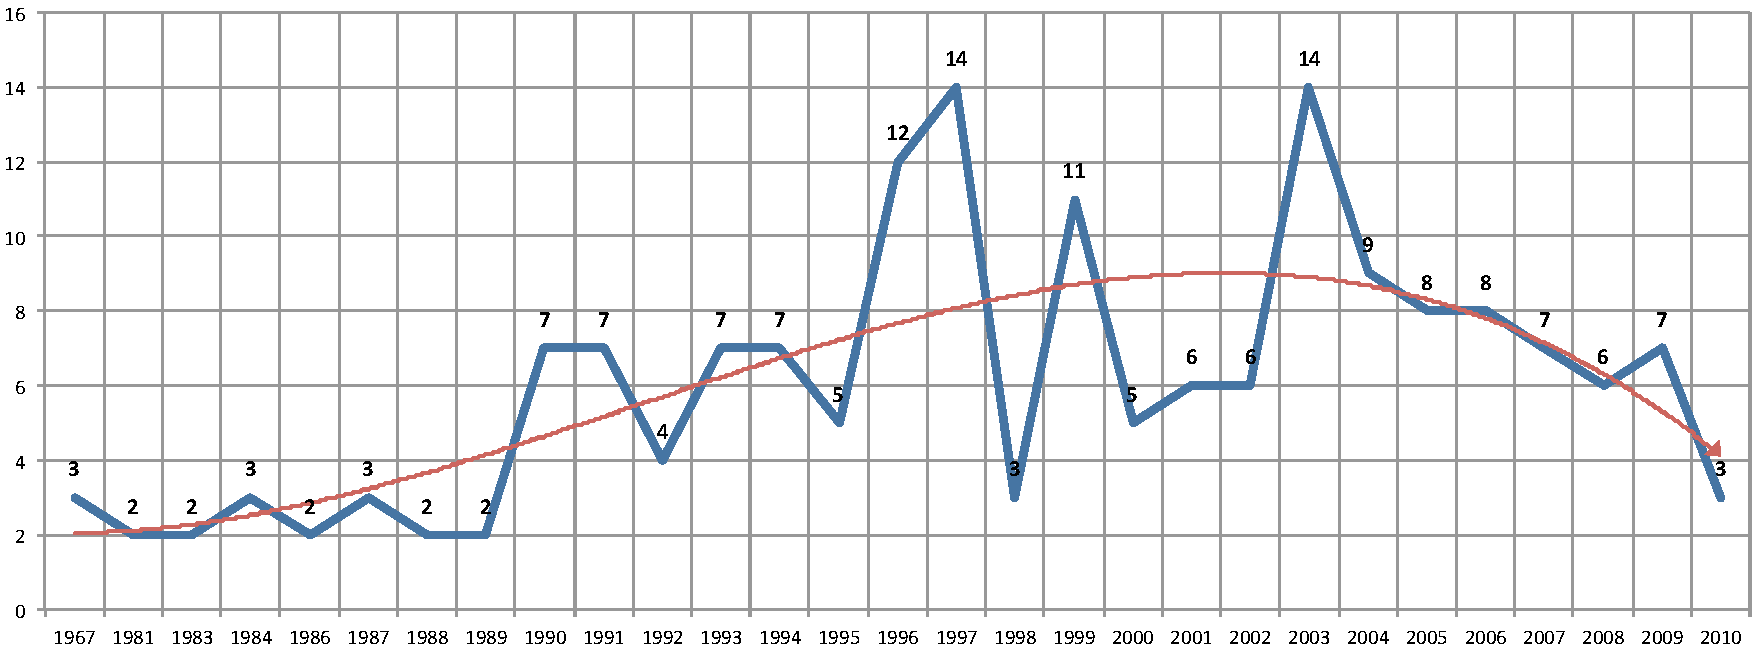
\includegraphics[scale=0.5]{abntex2-modelo-img-grafico.pdf}
	\end{center}
	\legend{Fonte: \citeonline[p. 24]{araujo2012}}
\end{figure}

% ---
\subsection{Figuras em \emph{minipages}}
% ---

\emph{Minipages} são usadas para inserir textos ou outros elementos em quadros
com tamanhos e posições controladas. Veja o exemplo da
\autoref{fig_minipage_imagem1} e da \autoref{fig_minipage_grafico2}.

\begin{figure}[htb]
 \label{teste}
 \centering
  \begin{minipage}{0.4\textwidth}
    \centering
    \caption{Imagem 1 da minipage} \label{fig_minipage_imagem1}
    
\includegraphics[scale=0.9]{abntex2-modelo-img-marca.pdf}
    \legend{Fonte: Produzido pelos autores}
  \end{minipage}
  \hfill
  \begin{minipage}{0.4\textwidth}
    \centering
    \caption{Grafico 2 da minipage} \label{fig_minipage_grafico2}
    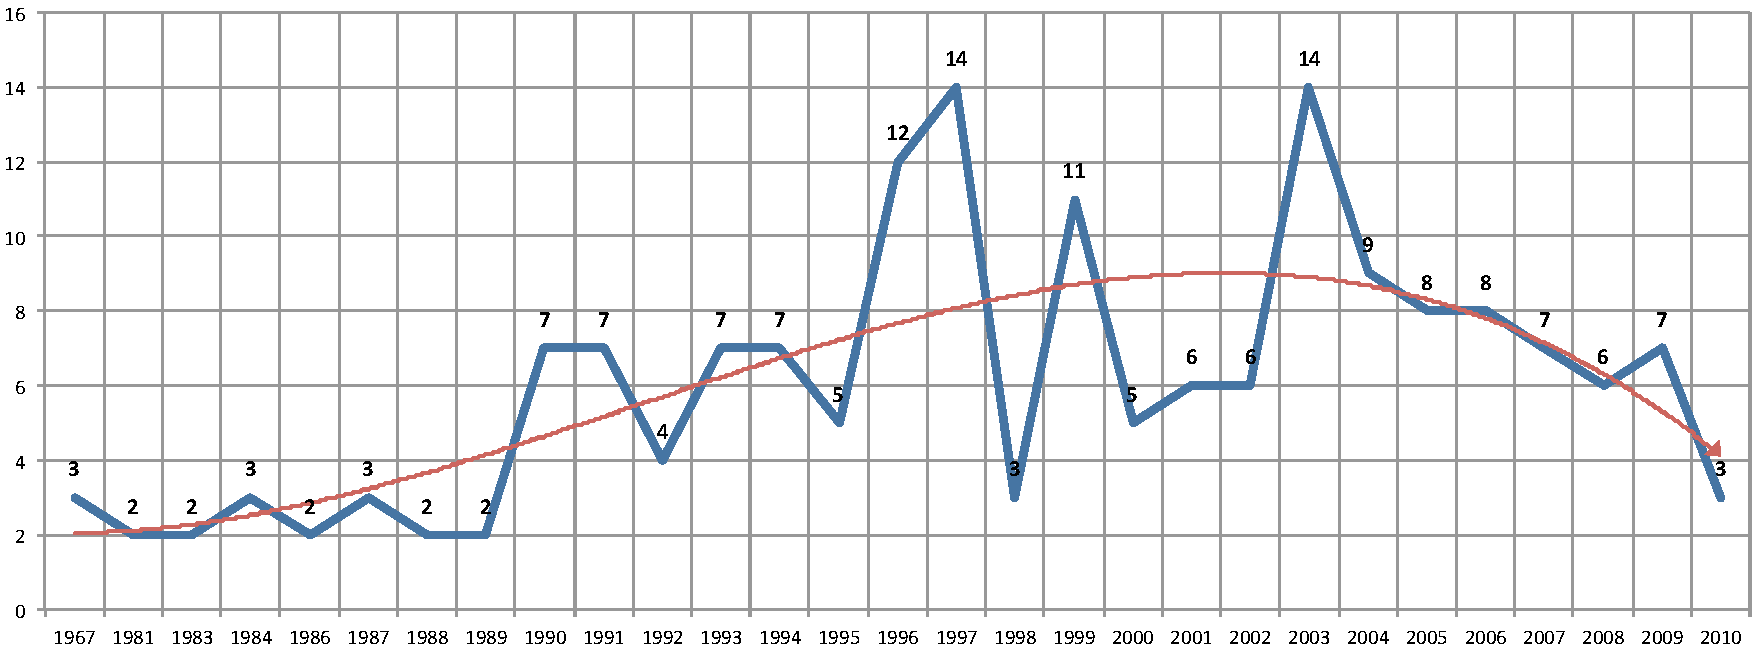
\includegraphics[scale=0.2]{abntex2-modelo-img-grafico.pdf}
    \legend{Fonte: \citeonline[p. 24]{araujo2012}}
  \end{minipage}
\end{figure}

Observe que, segundo a \citeonline[seções 4.2.1.10 e 5.8]{NBR14724:2011}, as
ilustrações devem sempre ter numeração contínua e única em todo o documento:

\begin{citacao}
Qualquer que seja o tipo de ilustração, sua identificação aparece na parte
superior, precedida da palavra designativa (desenho, esquema, fluxograma,
fotografia, gráfico, mapa, organograma, planta, quadro, retrato, figura,
imagem, entre outros), seguida de seu número de ordem de ocorrência no texto,
em algarismos arábicos, travessão e do respectivo título. Após a ilustração, na
parte inferior, indicar a fonte consultada (elemento obrigatório, mesmo que
seja produção do próprio autor), legenda, notas e outras informações
necessárias à sua compreensão (se houver). A ilustração deve ser citada no
texto e inserida o mais próximo possível do trecho a que se
refere. \cite[seções 5.8]{NBR14724:2011}
\end{citacao}

% ---
\section{Expressões matemáticas}
% ---

\index{expressões matemáticas}Use o ambiente \texttt{equation} para escrever
expressões matemáticas numeradas:

\begin{equation}
  \forall x \in X, \quad \exists \: y \leq \epsilon
\end{equation}

Escreva expressões matemáticas entre \$ e \$, como em $ \lim_{x \to \infty}
\exp(-x) = 0 $, para que fiquem na mesma linha.

Também é possível usar colchetes para indicar o início de uma expressão
matemática que não é numerada.

\[
\left|\sum_{i=1}^n a_ib_i\right|
\le
\left(\sum_{i=1}^n a_i^2\right)^{1/2}
\left(\sum_{i=1}^n b_i^2\right)^{1/2}
\]

Consulte mais informações sobre expressões matemáticas em
\url{https://github.com/abntex/abntex2/wiki/Referencias}.

% ---
\section{Enumerações: alíneas e subalíneas}
% ---

\index{alíneas}\index{subalíneas}\index{incisos}Quando for necessário enumerar
os diversos assuntos de uma seção que não possua título, esta deve ser
subdividida em alíneas \cite[4.2]{NBR6024:2012}:

\begin{alineas}

  \item os diversos assuntos que não possuam título próprio, dentro de uma mesma
  seção, devem ser subdivididos em alíneas; 
  
  \item o texto que antecede as alíneas termina em dois pontos;
  \item as alíneas devem ser indicadas alfabeticamente, em letra minúscula,
  seguida de parêntese. Utilizam-se letras dobradas, quando esgotadas as
  letras do alfabeto;

  \item as letras indicativas das alíneas devem apresentar recuo em relação à
  margem esquerda;

  \item o texto da alínea deve começar por letra minúscula e terminar em
  ponto-e-vírgula, exceto a última alínea que termina em ponto final;

  \item o texto da alínea deve terminar em dois pontos, se houver subalínea;

  \item a segunda e as seguintes linhas do texto da alínea começa sob a
  primeira letra do texto da própria alínea;
  
  \item subalíneas \cite[4.3]{NBR6024:2012} devem ser conforme as alíneas a
  seguir:

  \begin{alineas}
     \item as subalíneas devem começar por travessão seguido de espaço;

     \item as subalíneas devem apresentar recuo em relação à alínea;

     \item o texto da subalínea deve começar por letra minúscula e terminar em
     ponto-e-vírgula. A última subalínea deve terminar em ponto final, se não
     houver alínea subsequente;

     \item a segunda e as seguintes linhas do texto da subalínea começam sob a
     primeira letra do texto da própria subalínea.
  \end{alineas}
  
  \item no \abnTeX\ estão disponíveis os ambientes \texttt{incisos} e
  \texttt{subalineas}, que em suma são o mesmo que se criar outro nível de
  \texttt{alineas}, como nos exemplos à seguir:
  
  \begin{incisos}
    \item \textit{Um novo inciso em itálico};
  \end{incisos}
  
  \item Alínea em \textbf{negrito}:
  
  \begin{subalineas}
    \item \textit{Uma subalínea em itálico};
    \item \underline{\textit{Uma subalínea em itálico e sublinhado}}; 
  \end{subalineas}
  
  \item Última alínea com \emph{ênfase}.
  
\end{alineas}

% ---
\section{Espaçamento entre parágrafos e linhas}
% ---

\index{espaçamento!dos parágrafos}O tamanho do parágrafo, espaço entre a margem
e o início da frase do parágrafo, é definido por:

\begin{verbatim}
   \setlength{\parindent}{1.3cm}
\end{verbatim}

\index{espaçamento!do primeiro parágrafo}Por padrão, não há espaçamento no
primeiro parágrafo de cada início de divisão do documento
(\autoref{sec-divisoes}). Porém, você pode definir que o primeiro parágrafo
também seja indentado, como é o caso deste documento. Para isso, apenas inclua o
pacote \textsf{indentfirst} no preâmbulo do documento:

\begin{verbatim}
   \usepackage{indentfirst}      % Indenta o primeiro parágrafo de cada seção.
\end{verbatim}

\index{espaçamento!entre os parágrafos}O espaçamento entre um parágrafo e outro
pode ser controlado por meio do comando:

\begin{verbatim}
  \setlength{\parskip}{0.2cm}  % tente também \onelineskip
\end{verbatim}

\index{espaçamento!entre as linhas}O controle do espaçamento entre linhas é
definido por:

\begin{verbatim}
  \OnehalfSpacing       % espaçamento um e meio (padrão); 
  \DoubleSpacing        % espaçamento duplo
  \SingleSpacing        % espaçamento simples	
\end{verbatim}

Para isso, também estão disponíveis os ambientes:

\begin{verbatim}
  \begin{SingleSpace} ...\end{SingleSpace}
  \begin{Spacing}{hfactori} ... \end{Spacing}
  \begin{OnehalfSpace} ... \end{OnehalfSpace}
  \begin{OnehalfSpace*} ... \end{OnehalfSpace*}
  \begin{DoubleSpace} ... \end{DoubleSpace}
  \begin{DoubleSpace*} ... \end{DoubleSpace*} 
\end{verbatim}

Para mais informações, consulte \citeonline[p. 47-52 e 135]{memoir}.

% ---
\section{Inclusão de outros arquivos}\label{sec-include}
% ---

É uma boa prática dividir o seu documento em diversos arquivos, e não
apenas escrever tudo em um único. Esse recurso foi utilizado neste
documento. Para incluir diferentes arquivos em um arquivo principal,
de modo que cada arquivo incluído fique em uma página diferente, utilize o
comando:

\begin{verbatim}
   \include{documento-a-ser-incluido}      % sem a extensão .tex
\end{verbatim}

Para incluir documentos sem quebra de páginas, utilize:

\begin{verbatim}
   \input{documento-a-ser-incluido}      % sem a extensão .tex
\end{verbatim}

% ---
\section{Compilar o documento \LaTeX}
% ---

Geralmente os editores \LaTeX, como o
TeXlipse\footnote{\url{http://texlipse.sourceforge.net/}}, o
Texmaker\footnote{\url{http://www.xm1math.net/texmaker/}}, entre outros,
compilam os documentos automaticamente, de modo que você não precisa se
preocupar com isso.

No entanto, você pode compilar os documentos \LaTeX usando os seguintes
comandos, que devem ser digitados no \emph{Prompt de Comandos} do Windows ou no
\emph{Terminal} do Mac ou do Linux:

\begin{verbatim}
   pdflatex ARQUIVO_PRINCIPAL.tex
   bibtex ARQUIVO_PRINCIPAL.aux
   makeindex ARQUIVO_PRINCIPAL.idx 
   makeindex ARQUIVO_PRINCIPAL.nlo -s nomencl.ist -o ARQUIVO_PRINCIPAL.nls
   pdflatex ARQUIVO_PRINCIPAL.tex
   pdflatex ARQUIVO_PRINCIPAL.tex
\end{verbatim}

% ---
\section{Remissões internas}
% ---

Ao nomear a \autoref{tab-nivinv} e a \autoref{fig_circulo}, apresentamos um
exemplo de remissão interna, que também pode ser feita quando indicamos o
\autoref{cap_exemplos}, que tem o nome \emph{\nameref{cap_exemplos}}. O número
do capítulo indicado é \ref{cap_exemplos}, que se inicia à
\autopageref{cap_exemplos}\footnote{O número da página de uma remissão pode ser
obtida também assim:
\pageref{cap_exemplos}.}.
Veja a \autoref{sec-divisoes} para outros exemplos de remissões internas entre
seções, subseções e subsubseções.

O código usado para produzir o texto desta seção é:

\begin{verbatim}
Ao nomear a \autoref{tab-nivinv} e a \autoref{fig_circulo}, apresentamos um
exemplo de remissão interna, que também pode ser feita quando indicamos o
\autoref{cap_exemplos}, que tem o nome \emph{\nameref{cap_exemplos}}. O número
do capítulo indicado é \ref{cap_exemplos}, que se inicia à
\autopageref{cap_exemplos}\footnote{O número da página de uma remissão pode ser
obtida também assim:
\pageref{cap_exemplos}.}.
Veja a \autoref{sec-divisoes} para outros exemplos de remissões internas entre
seções, subseções e subsubseções.
\end{verbatim}

% ---
\section{Divisões do documento: seção}\label{sec-divisoes}
% ---

Esta seção testa o uso de divisões de documentos. Esta é a
\autoref{sec-divisoes}. Veja a \autoref{sec-divisoes-subsection}.

\subsection{Divisões do documento: subseção}\label{sec-divisoes-subsection}

Isto é uma subseção. Veja a \autoref{sec-divisoes-subsubsection}, que é uma
\texttt{subsubsection} do \LaTeX, mas é impressa chamada de ``subseção'' porque
no Português não temos a palavra ``subsubseção''.

\subsubsection{Divisões do documento: subsubseção}
\label{sec-divisoes-subsubsection}

Isto é uma subsubseção.

\subsubsection{Divisões do documento: subsubseção}

Isto é outra subsubseção.

\subsection{Divisões do documento: subseção}\label{sec-exemplo-subsec}

Isto é uma subseção.

\subsubsection{Divisões do documento: subsubseção}

Isto é mais uma subsubseção da \autoref{sec-exemplo-subsec}.


\subsubsubsection{Esta é uma subseção de quinto
nível}\label{sec-exemplo-subsubsubsection}

Esta é uma seção de quinto nível. Ela é produzida com o seguinte comando:

\begin{verbatim}
\subsubsubsection{Esta é uma subseção de quinto
nível}\label{sec-exemplo-subsubsubsection}
\end{verbatim}

\subsubsubsection{Esta é outra subseção de quinto nível}\label{sec-exemplo-subsubsubsection-outro}

Esta é outra seção de quinto nível.


\paragraph{Este é um parágrafo numerado}\label{sec-exemplo-paragrafo}

Este é um exemplo de parágrafo nomeado. Ele é produzida com o comando de
parágrafo:

\begin{verbatim}
\paragraph{Este é um parágrafo nomeado}\label{sec-exemplo-paragrafo}
\end{verbatim}

A numeração entre parágrafos numeradaos e subsubsubseções são contínuas.

\paragraph{Esta é outro parágrafo numerado}\label{sec-exemplo-paragrafo-outro}

Esta é outro parágrafo nomeado.

% ---
\section{Este é um exemplo de nome de seção longo. Ele deve estar
alinhado à esquerda e a segunda e demais linhas devem iniciar logo abaixo da
primeira palavra da primeira linha}
% ---

Isso atende à norma \citeonline[seções de 5.2.2 a 5.2.4]{NBR14724:2011} 
 e \citeonline[seções de 3.1 a 3.8]{NBR6024:2012}.

% ---
\section{Diferentes idiomas e hifenizações}
\label{sec-hifenizacao}
% ---

Para usar hifenizações de diferentes idiomas, inclua nas opções do documento o
nome dos idiomas que o seu texto contém. Por exemplo (para melhor
visualização, as opções foram quebras em diferentes linhas):

\begin{verbatim}
\documentclass[
	12pt,
	openright,
	twoside,
	a4paper,
	english,
	french,
	spanish,
	brazil
	]{abntex2}
\end{verbatim}

O idioma português-brasileiro (\texttt{brazil}) é incluído automaticamente pela
classe \textsf{abntex2}. Porém, mesmo assim a opção \texttt{brazil} deve ser
informada como a última opção da classe para que todos os pacotes reconheçam o
idioma. Vale ressaltar que a última opção de idioma é a utilizada por padrão no
documento. Desse modo, caso deseje escrever um texto em inglês que tenha
citações em português e em francês, você deveria usar o preâmbulo como abaixo:

\begin{verbatim}
\documentclass[
	12pt,
	openright,
	twoside,
	a4paper,
	french,
	brazil,
	english
	]{abntex2}
\end{verbatim}

A lista completa de idiomas suportados, bem como outras opções de hifenização,
estão disponíveis em \citeonline[p.~5-6]{babel}.

Exemplo de hifenização em inglês\footnote{Extraído de:
\url{http://en.wikibooks.org/wiki/LaTeX/Internationalization}}:

\begin{otherlanguage*}{english}
\textit{Text in English language. This environment switches all language-related
definitions, like the language specific names for figures, tables etc. to the other
language. The starred version of this environment typesets the main text
according to the rules of the other language, but keeps the language specific
string for ancillary things like figures, in the main language of the document.
The environment hyphenrules switches only the hyphenation patterns used; it can
also be used to disallow hyphenation by using the language name
`nohyphenation'.}
\end{otherlanguage*}

Exemplo de hifenização em francês\footnote{Extraído de:
\url{http://bigbrowser.blog.lemonde.fr/2013/02/17/tu-ne-tweeteras-point-le-vatican-interdit-aux-cardinaux-de-tweeter-pendant-le-conclave/}}:

\begin{otherlanguage*}{french}
\textit{Texte en français. Pas question que Twitter ne vienne faire une
concurrence déloyale à la traditionnelle fumée blanche qui marque l'élection
d'un nouveau pape. Pour éviter toute fuite précoce, le Vatican a donc pris un
peu d'avance, et a déjà interdit aux cardinaux qui prendront part au vote
d'utiliser le réseau social, selon Catholic News Service. Une mesure valable
surtout pour les neuf cardinaux – sur les 117 du conclave – pratiquants très
actifs de Twitter, qui auront interdiction pendant toute la période de se
connecter à leur compte.}
\end{otherlanguage*}

Pequeno texto em espanhol\footnote{Extraído de:
\url{http://internacional.elpais.com/internacional/2013/02/17/actualidad/1361102009_913423.html}}:

\foreignlanguage{spanish}{\textit{Decenas de miles de personas ovacionan al pontífice en su
penúltimo ángelus dominical, el primero desde que anunciase su renuncia. El Papa se
centra en la crítica al materialismo}}.

O idioma geral do texto por ser alterado como no exemplo seguinte:

\begin{verbatim}
  \selectlanguage{english}
\end{verbatim}

Isso altera automaticamente a hifenização e todos os nomes constantes de
referências do documento para o idioma inglês. Consulte o manual da classe
\cite{abntex2classe} para obter orientações adicionais sobre internacionalização de
documentos produzidos com \abnTeX.

A \autoref{sec-citacao} descreve o ambiente \texttt{citacao} que pode receber
como parâmetro um idioma a ser usado na citação.

% ---
\section{Consulte o manual da classe \textsf{abntex2}}
% ---

Consulte o manual da classe \textsf{abntex2} \cite{abntex2classe} para uma
referência completa das macros e ambientes disponíveis. 

Além disso, o manual possui informações adicionais sobre as normas ABNT
observadas pelo \abnTeX\ e considerações sobre eventuais requisitos específicos
não atendidos, como o caso da \citeonline[seção 5.2.2]{NBR14724:2011}, que
especifica o espaçamento entre os capítulos e o início do texto, regra
propositalmente não atendida pelo presente modelo.

% ---
\section{Referências bibliográficas}
% ---

A formatação das referências bibliográficas conforme as regras da ABNT são um
dos principais objetivos do \abnTeX. Consulte os manuais
\citeonline{abntex2cite} e \citeonline{abntex2cite-alf} para obter informações
sobre como utilizar as referências bibliográficas.

%-
\subsection{Acentuação de referências bibliográficas}
%-

Normalmente não há problemas em usar caracteres acentuados em arquivos
bibliográficos (\texttt{*.bib}). Porém, como as regras da ABNT fazem uso quase
abusivo da conversão para letras maiúsculas, é preciso observar o modo como se
escreve os nomes dos autores. Na ~\autoref{tabela-acentos} você encontra alguns
exemplos das conversões mais importantes. Preste atenção especial para `ç' e `í'
que devem estar envoltos em chaves. A regra geral é sempre usar a acentuação
neste modo quando houver conversão para letras maiúsculas.

\begin{table}[htbp]
\caption{Tabela de conversão de acentuação.}
\label{tabela-acentos}

\begin{center}
\begin{tabular}{ll}\hline\hline
acento & \textsf{bibtex}\\
à á ã & \verb+\`a+ \verb+\'a+ \verb+\~a+\\
í & \verb+{\'\i}+\\
ç & \verb+{\c c}+\\
\hline\hline
\end{tabular}
\end{center}
\end{table}


% ---
\section{Precisa de ajuda?}
% ---

Consulte a FAQ com perguntas frequentes e comuns no portal do \abnTeX:
\url{https://github.com/abntex/abntex2/wiki/FAQ}.

Inscreva-se no grupo de usuários \LaTeX:
\url{http://groups.google.com/group/latex-br}, tire suas dúvidas e ajude
outros usuários.

Participe também do grupo de desenvolvedores do \abnTeX:
\url{http://groups.google.com/group/abntex2} e faça sua contribuição à
ferramenta.

% ---
\section{Você pode ajudar?}
% ---

Sua contribuição é muito importante! Você pode ajudar na divulgação, no
desenvolvimento e de várias outras formas. Veja como contribuir com o \abnTeX\
em \url{https://github.com/abntex/abntex2/wiki/Como-Contribuir}.

% ---
\section{Quer customizar os modelos do \abnTeX\ para sua instituição ou
universidade?}
% ---

Veja como customizar o \abnTeX\ em:
\url{https://github.com/abntex/abntex2/wiki/ComoCustomizar}.


% ---

% ----------------------------------------------------------
% PARTE
% ----------------------------------------------------------
\part{Literature Review}
% ----------------------------------------------------------
%% abtex2-modelo-include-comandos.tex, v-1.9.5 laurocesar
%% Copyright 2012-2015 by abnTeX2 group at http://www.abntex.net.br/ 
%%
%% This work may be distributed and/or modified under the
%% conditions of the LaTeX Project Public License, either version 1.3
%% of this license or (at your option) any later version.
%% The latest version of this license is in
%%   http://www.latex-project.org/lppl.txt
%% and version 1.3 or later is part of all distributions of LaTeX
%% version 2005/12/01 or later.
%%
%% This work has the LPPL maintenance status `maintained'.
%% 
%% The Current Maintainer of this work is the abnTeX2 team, led
%% by Lauro César Araujo. Further information are available on 
%% http://www.abntex.net.br/
%%
%% This work consists of the files abntex2-modelo-include-comandos.tex
%% and abntex2-modelo-img-marca.pdf
%%

% ---
% Este capítulo, utilizado por diferentes exemplos do abnTeX2, ilustra o uso de
% comandos do abnTeX2 e de LaTeX.
% ---
 
\chapter{Background}\label{background}
\chapterprecis{The purpose of this section is to understand the problem.}\index{sinopse de capítulo}

% ---
\section{Similar Selection Systems}
% ---

\noindent
An optimization procedure which is similar to ours is presented by \cite{raynersss13}, but their procedure maximizes the average heuristic value. By contrast, the meta$-$reasoning we are proposing minimizes the search tree size.\\

Our meta$-$reasoning requires a prediction of the number of nodes expanded by A$\sp{*}$ using any given subset. Although there are methods for accurately predicting the number of nodes expanded by Iterative Deepening$-$A$\sp{*}$ \cite{Korf85ida} (ID$A\sp{*}$). (\texttt{SS} system  \cite{lelis2013predicting}), these methods can't be easily adapted to A$\sp{*}$ because A$\sp{*}$'s duplicate pruning makes it very difficult to predict how many nodes will occur at depth $d$ of $A\sp{*}$'s search tree (the tree of nodes expanded by $A\sp{*}$). As a part of our proposal, we present \texttt{SS} for predicting the size of the search tree.

The system most similar to ours is \textbf{RIDA$\sp{*}$} \cite{BarleySantiagoOver}. \textbf{RIDA$\sp{*}$} also selects a subset from a pool of heuristics to guide the $A\sp{*}$ search. In \textbf{RIDA$\sp{*}$} this is done by starting with an empty subset and trying all combination of size one before trying the combination of size two and so on. \textbf{RIDA$\sp{*}$} stops after evaluating a fixed number of subsets. While \textbf{RIDA$\sp{*}$} is able to evaluate a set of heuristics with tens of elements, our meta$-$reasoning is able to evaluate a set of heuristics with thousands of elements.

% ---
\section{Problem definition}
% ---

A $SAS\sp{+} planning\ task$ \cite{backstrom1995complexity} is a 4 tuple $\triangledown = \{V, O, I, G\}.$ \textit{V} is a set of \textit{state variables.} Each variable \textit{v} $\in$ \textit{V} is associated with a finite domain of possible $D_{\substack{v}}$. A state is an assignment of a value to every $v \in V.$ The set of possible states, denoted \textit{V}, is therefore $D_{\substack{v_{\substack{1}}}}    \times ... \times D_{\substack{v_{\substack{2}}}}$. \textit{O} is a set of operators, where each operator $o \in O$ is triple $\{pre_{\substack{o}} , post_{\substack{o}}, cost_{\substack{o}}\}$ specifying the preconditions, postconditions (effects), and non-negative cost of \textit{o}. $pre_{\substack{o}}\ and\ post_{\substack{o}}$ are assignments of values to subsets os variables, $V_{\substack{pre_{\substack{o}}}}\ and\ V_{\substack{post_{\substack{o}}}}$, respectively. Operator \textit{o} is applicable to state \textit{s} if \textit{s} and $pre_{\substack{o}}$ agree on the assignment of values to variables in $V_{\substack{pre_{\substack{o}}}}$. The effect of \textit{o}, when applied to \textit{s}, is to set the variables in $V_{\substack{post_{\substack{o}}}}$ to the values specified in $post_{\substack{o}}$ and to set all other variables to the value they have in \textit{s}. \textit{G} is the goal condition, an assignment of values to a subset of variables, $V_{\substack{G}}$. A state is a goal state if it and \textit{G} agree on the assignment of values to the variable in $V_{\substack{G}}$. \textit{I} is the initial state, and the planning task, $\triangledown$, is to find an optimal (least-cost) sequence of operators leading from \textit{I} to a goal state. We denote the optimal solution cost of $\triangledown$ as $C\sp{*}$ \\

The state space problem illustrated in the figure \ref{fig:8tilepuzzle_begin} is a game that consists of a frame of numbered square tiles in random order with one tile missing. The puzzle also exists in other sizes, particularly the smaller 8$-$puzzle. If the size is 3$\times$3 tiles, the puzzle is called the 8$-$puzzle or 9$-$puzzle, and if 4 $\times$ 4 tiles, the puzzle is called the 15$-$puzzle or 16$-$puzzle named, respectively, for the number of tiles and the number of spaces. The object of the puzzle is to place the tiles in order by making sliding moves that use the empty space. \\

The legal operators are to slide any tile that is horizontally or vertically adjacent to the blank into the blank position. The problem is to rearrange the tiles from some random initial configuration into a particular desired goal configuration. The 8$-$puzzle contains 181,440 reachable states, the 15$-$puzzle contains about $10\sp{13}$ reachable states, and the 24$-$puzzle contains almost $10\sp{25}$ states. \\

\begin{figure}[htb]
\centering
\begin{forest}
 [\usebox\myboxa \hspace*{1.4in} \usebox\myboxb]
 $\node [xshift=-5.5cm,yshift=3.5cm] (A) at (2,0) {Initial};$
 $\node [xshift=1.5cm,yshift=3.5cm] (A) at (2,0) {Goal};$
\end{forest}
\caption{The left tile$-$puzzle is the initial distribution of tiles and the right tile$-$puzzle is the goal distribution of tiles. Each one represent a State.} \label{fig:8tilepuzzle_begin}
\end{figure}


Instead of using an algorithm of Brute force search that will analyze all the possible solutions. We can obtain heuristics from the problem of the slide tile puzzle that will help us to solve the problem.

\section{Heuristics}
State$-$space algorithms, such as A* \cite{hart1968formal}, are important in many \texttt{AI} applications. A* uses the $f(s) = g(s) + h(s)$ cost function to guide its search. Here, $g(s)$ is the cost of the path from the start state $s$, and $h(s)$ is the estimated cost$-$to$-$go from $s$ to a gial; $h(.)$ is known as the heuristic function. The heuristic is the mathematical concept that represent to the estimate distance from the node $s$ to the nearest goal state.

\begin{figure}[htb]
\centering
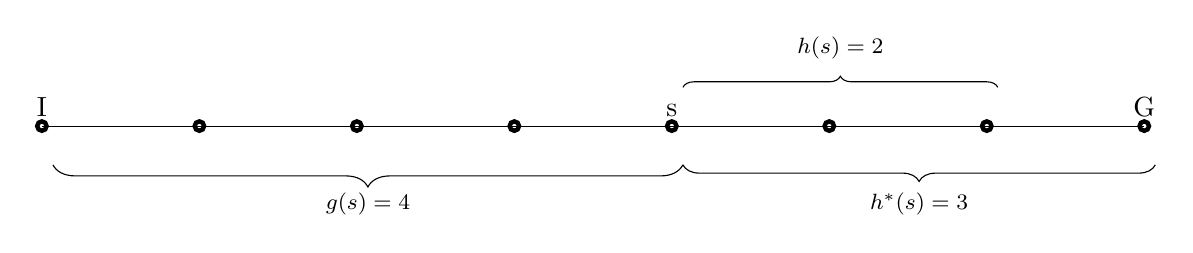
\begin{tikzpicture}
	%\draw[yshift=-1 em, ultra thick] (0,0) [point] -- (5,0) [point] -- (10,0) [point];
	\coordinate (I) at (0,0) (I) node[point=ultra thick, above] {I};
	\coordinate (I1) at (2,0) (I1) node[point=ultra thick, above] {};
	\coordinate (I2) at (4,0) (I2) node[point=ultra thick, above] {};
	\coordinate (I3) at (6,0) (I3) node[point=ultra thick, above] {};
	\coordinate (s) at (8,0) (s) node[point=ultra thick, above] {s};
	\coordinate (I4) at (10,0) (I4) node[point=ultra thick, above] {};
	\coordinate (I5) at (12,0) (I5) node[point=ultra thick, above] {};
	\coordinate (G) at (14,0) (G) node[point=ultra thick, above] {G};
	\draw (I) -- (G);	

\draw [decorate,decoration={brace,amplitude=4pt},xshift=4pt,yshift=14pt]
(8,0) -- (12,0) node [black,midway,yshift=0.5cm] 
{\footnotesize $h(s)=2$};

\draw [decorate,decoration={brace,amplitude=8pt,mirror},xshift=4pt,yshift=-14pt]
(0,0) -- (8,0) node [black,midway,yshift=-0.5cm] 
{\footnotesize $g(s)=4$};


\draw [decorate,decoration={brace,amplitude=6pt,mirror},xshift=4pt,yshift=-14pt]
(8,0) -- (14,0) node [black,midway,yshift=-0.5cm] 
{\footnotesize $h\sp{*}(s)=3$};
\end{tikzpicture}
\caption{Heuristic Search: \textit{I}: Initial State, \textit{s}: Some Sate, \textit{G}: Goal State} \label{fig:searchSpace}
\end{figure}

In the figure \ref{fig:searchSpace} the optimal distance from the Initial State $I$ to  the state $s$ is 4 and represented by $g(s)$. The $h\sp{*}(s)$ represent the optimal distance from $s$ to the Goal State $G$. And the $h(s)$ is the estimation distance from $s$ to $G$.

A heuristic function $h(s)$ estimates the cost of a solution path from $s$ to a goal state. A heuristic is admissible if $h(s) \leq h\sp{*}(s)$ for all $s \in V$, where $h\sp{*}(s)$ is the optimal cost of $s$. A heuristic is consisten iff $h(s) \leq c(s,t) + h(t)$ for all states $s$ and $t$, where $c(s,t)$ is the cost of the cheapest path from $s$ to $t$. For example, the heuristic function provided by a pattern database (\texttt{PDB}) heuristic \cite{culberson1998pattern} is admissible and consistent.

Given a set of admissible and consistent heuristics $\zeta = \{h_{1}, h_{2}, \dots, h_{M}\}$, the heuristic $h_{max}(s,\zeta) = $max$_{h \in \zeta} h(s)$ is also admissible and consistent. When describing our method we assume all heuristics to be consistent. We define $f_{max}(s, \zeta) = g(s) + h_{max}(s, \zeta)$, where $g(s)$ is the cost of the path expanded from $I$ to $s$. $g(s)$ is minimal when A$\sp{*}$ using a consistent heuristic expands $s$. We call an A$\sp{*}$ search tree the tree defined by the states expanded by A$\sp{*}$ using a consistent heuristic while solving a problem $\triangledown$.

The heuristics can be obtained from each state of the problem. For example, for the problem of the 8$-$tile$-$puzzle figure \ref{fig:8tilepuzzle_begin} we can get two heuristics.

\subsection{Out of place (O.P)}
Counts the number of objects out of place.

\begin{figure}[htb]
\centering
\begin{forest}
 [\usebox\myboxa]
 $\draw[->,xshift=4pt,yshift=14pt] (2,1) -- (4,1);$
 $\node [xshift=1cm,yshift=2cm] (A) at (2,0) {O.P=8};$
 \hspace*{1.8in} 
 %$\rightarrow$  
 [\usebox\myboxb] 
\end{forest}
\caption{Out of place heuristic} \label{fig:8tilepuzzle_oop}
\end{figure}

The tiles numbered with 4, 1, 2, 3, 6, 7, 5, 8, and 4 are out of place then each object count as 1 and the sum would be 8.

\subsection{Manhatham Distance (M.D)}
Counts the minimum number of operations to get to the goal state.

\begin{figure}[htb]
\centering
\begin{forest}
 [\usebox\myboxa]
 $\draw[->,xshift=4pt,yshift=14pt] (2,1) -- (4,1);$
 $\node [xshift=1cm,yshift=2cm] (A) at (2,0) {M.D=1O};$
 \hspace*{1.8in} 
 %$\rightarrow$  
 [\usebox\myboxb] 
\end{forest}
\caption{Manhatham distance heuristic} \label{fig:8tilepuzzle_md}
\end{figure}

The tile 4 count 1 to get to the goal position.
The tile 1 count 1 to get to the goal position.
The tile 2 count 1 to get to the goal position.
The tile 3 count 1 to get to the goal position.
The tile 6 count 1 to get to the goal position.
The tile 7 count 1 to get to the goal position.
The tile 5 count 1 to get to the goal position.
The tile 8 count 1 to get to the goal position.
Then the sum would be 10.

In order to solve the problem, we get the heuristics, which are information from the problem to solve the problem. Exists systems that can create heuristics for each problem. Those systems are called Heuristic Generators.

\section{Heuristic Generators}
Heuristic Generators works by creating abstractions of the original problem space. The approach that has showed more successful results lately is \texttt{PDB}.

\subsection{Pattern Database (PDB)}
It's obtained by abstracting away certain problem variables, so that the remaining problem ("pattern") is small enough to be solved optimally for every state by blind exhaustive search. The results stored in a table, represent a PDB for the original problem. The abstraction of the search space gives an admissible heuristic function, mapping states to lower bounds.

\section{Take advantage of Heuristics}
The heuristics generators can create hundreds or even thousand of heuristics. In fact, exists different ways to take advantage of those heuristics. For example: If we want to use all the heuristics created by the heuristic generator. It would not be a good idea to use all of them because the main problem involved would be the time to evaluate each heuristic in the search tree, it could take too much time. \\

One way to take advantage of heuristics would be to take the maximum of the set of heuristics. For example, using three different heuristics $h1, h2$ and max($h1, h2$). Heuristic $h1$ and $h2$ are based on domain abstractions and the max($h1, h2$) is the maximum heuristic value of $h1$ and $h2$. \\

Exists different approaches to take advantage from a large set of heuristics. In this dissertation we use the meta$-$reasoning based on the minimum evaluation time. \\


\section{Number of heuristics created}
Let's suppose we have to run our meta$-$reasoning using M amount of memory available. The question would be: How many heuristics our system should handle in order to avoid out of memory errors? So. one of the objectives of this tesis is to find the number of heuristics that our subset $\zeta\sp{'}$ should have.

\begin{figure}[htb]
  \centering
  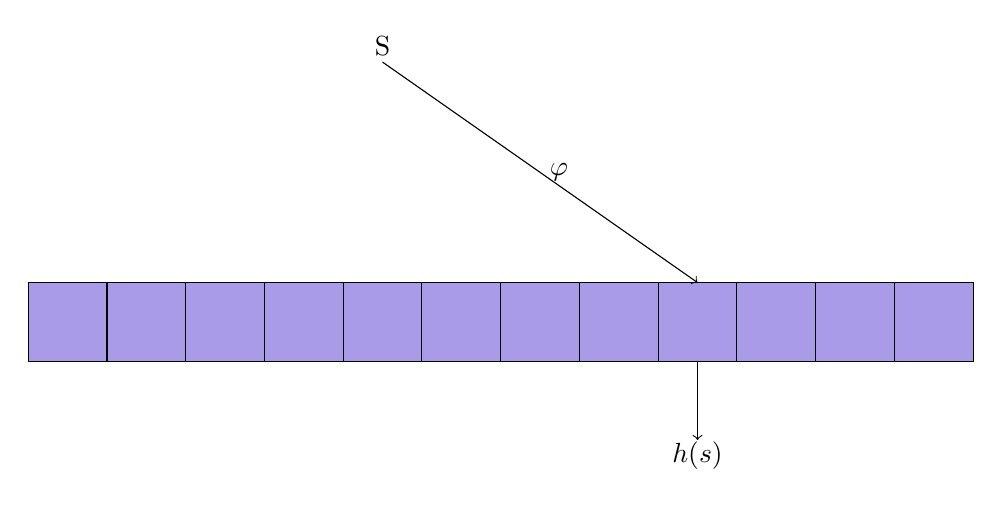
\begin{tikzpicture}
\draw[step=1cm,gray,very thin] grid (12,1);
%\draw[step=1cm,gray,very thin] (-1.9,-1.9) grid (5.9,5.9);
%\fill[blue!40!white] (0,0) rectangle (4,4);
\filldraw[fill=blue!40!white, draw=black] rectangle (12,1);
\filldraw[fill=blue!40!white, draw=black] rectangle (11,1);
\filldraw[fill=blue!40!white, draw=black] rectangle (10,1);
\filldraw[fill=blue!40!white, draw=black] rectangle (9,1);
\filldraw[fill=blue!40!white, draw=black] rectangle (8,1);
\filldraw[fill=blue!40!white, draw=black] rectangle (7,1);
\filldraw[fill=blue!40!white, draw=black] rectangle (6,1);
\filldraw[fill=blue!40!white, draw=black] rectangle (5,1);
\filldraw[fill=blue!40!white, draw=black] rectangle (4,1);
\filldraw[fill=blue!40!white, draw=black] rectangle (3,1);
\filldraw[fill=blue!40!white, draw=black] rectangle (2,1);
\filldraw[fill=blue!40!white, draw=black] rectangle (1,1);

 %$\draw[->,xshift=4pt,yshift=14pt] (2,1) -- (4,1);$
 \node [xshift=2.5cm,yshift=4cm] (A) at (2,0) {S};
 
 %\draw[->] (2.5cm,8em) -- (8cm,5em) node[midway,right] {\Om{2}};
 \draw[->] (4.5,3.8) -- (8.5,1) node[midway,right] {\Vpi{}};
 \draw[->] (8.5,0) -- (8.5,-1) node[xshift=0cm,yshift=-0.2cm] {$h(s)$};
\end{tikzpicture}
  \caption{One heuristic of size M}\label{fig:image1mem}
\end{figure}

\begin{figure}[htb]
  \centering
  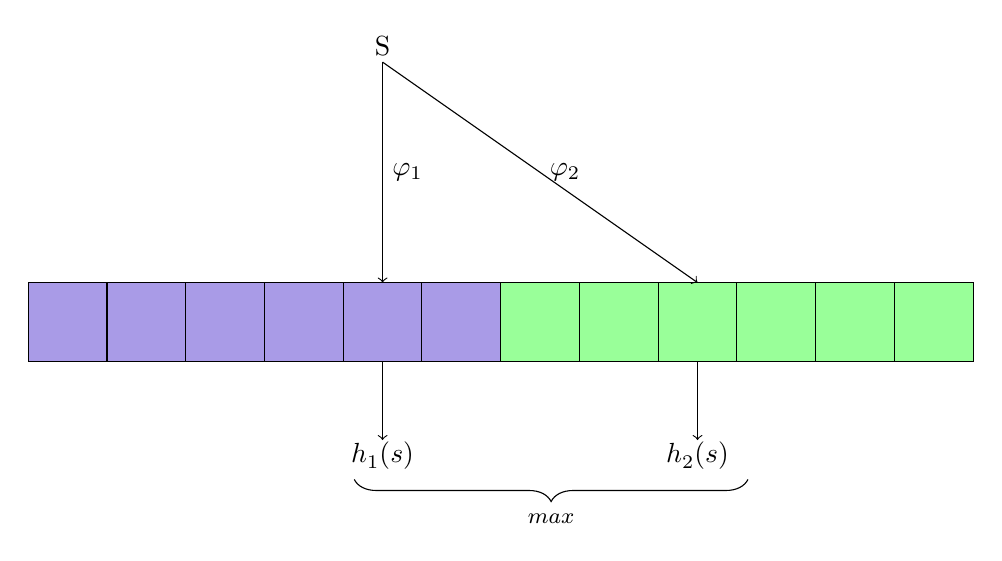
\begin{tikzpicture}
\draw[step=1cm,gray,very thin] grid (12,1);
%\draw[step=1cm,gray,very thin] (-1.9,-1.9) grid (5.9,5.9);
%\fill[blue!40!white] (0,0) rectangle (4,4);
\filldraw[fill=green!40!white, draw=black] rectangle (12,1);
\filldraw[fill=green!40!white, draw=black] rectangle (11,1);
\filldraw[fill=green!40!white, draw=black] rectangle (10,1);
\filldraw[fill=green!40!white, draw=black] rectangle (9,1);
\filldraw[fill=green!40!white, draw=black] rectangle (8,1);
\filldraw[fill=green!40!white, draw=black] rectangle (7,1);
\filldraw[fill=blue!40!white, draw=black] rectangle (6,1);
\filldraw[fill=blue!40!white, draw=black] rectangle (5,1);
\filldraw[fill=blue!40!white, draw=black] rectangle (4,1);
\filldraw[fill=blue!40!white, draw=black] rectangle (3,1);
\filldraw[fill=blue!40!white, draw=black] rectangle (2,1);
\filldraw[fill=blue!40!white, draw=black] rectangle (1,1);

 %$\draw[->,xshift=4pt,yshift=14pt] (2,1) -- (4,1);$
 \node [xshift=2.5cm,yshift=4cm] (A) at (2,0) {S};
 
 %\draw[->] (2.5cm,8em) -- (8cm,5em) node[midway,right] {\Om{2}};
 \draw[->] (4.5,3.8) -- (4.5,1) node[midway,right] {\Vpi{1}};
 \draw[->] (4.5,0) -- (4.5,-1) node[xshift=0cm,yshift=-0.2cm] {$h_{\substack{1}}(s)$};
 
 \draw[->] (4.5,3.8) -- (8.5,1) node[midway,right] {\Vpi{2}};
 \draw[->] (8.5,0) -- (8.5,-1) node[xshift=0cm,yshift=-0.2cm] {$h_{\substack{2}}(s)$};
 
 \draw[decorate,decoration={brace,amplitude=8pt,mirror},xshift=4pt,yshift=-1.5cm]
(4,0) -- (9,0) node [black,midway,yshift=-0.5cm] 
{\footnotesize $max$};
\end{tikzpicture}
  \caption{Two heuristics of size M/2}\label{fig:image2mem}
\end{figure}

\begin{figure}[htb]
  \centering
  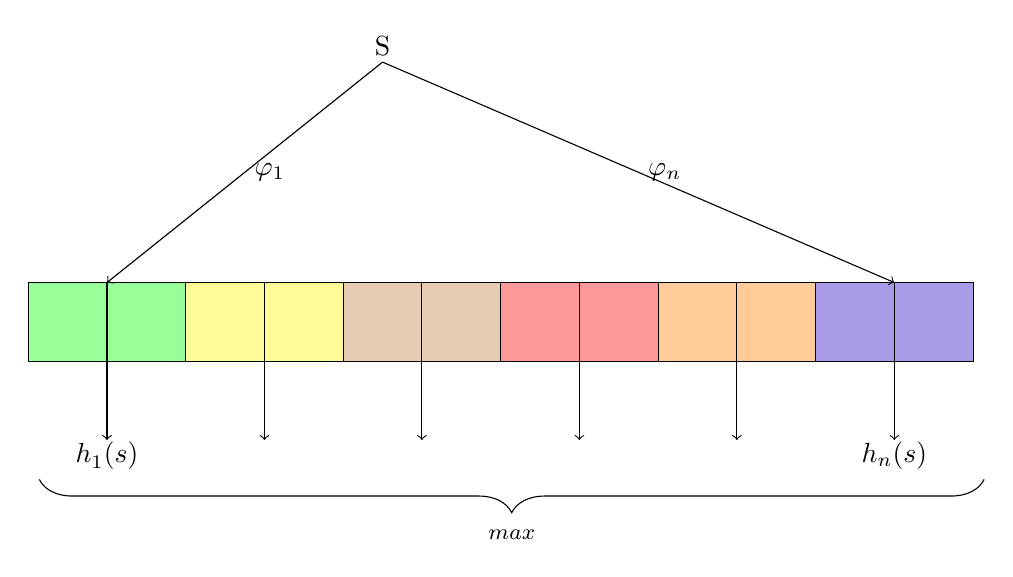
\begin{tikzpicture}
\draw[step=1cm,gray,very thin] grid (12,1);
%\draw[step=1cm,gray,very thin] (-1.9,-1.9) grid (5.9,5.9);
%\fill[blue!40!white] (0,0) rectangle (4,4);
\filldraw[fill=blue!40!white, draw=black] rectangle (12,1);
\filldraw[fill=blue!40!white, draw=black] rectangle (11,1);
\filldraw[fill=orange!40!white, draw=black] rectangle (10,1);
\filldraw[fill=orange!40!white, draw=black] rectangle (9,1);
\filldraw[fill=red!40!white, draw=black] rectangle (8,1);
\filldraw[fill=red!40!white, draw=black] rectangle (7,1);
\filldraw[fill=brown!40!white, draw=black] rectangle (6,1);
\filldraw[fill=brown!40!white, draw=black] rectangle (5,1);
\filldraw[fill=yellow!40!white, draw=black] rectangle (4,1);
\filldraw[fill=yellow!40!white, draw=black] rectangle (3,1);
\filldraw[fill=green!40!white, draw=black] rectangle (2,1);
\filldraw[fill=green!40!white, draw=black] rectangle (1,1);

 %$\draw[->,xshift=4pt,yshift=14pt] (2,1) -- (4,1);$
 \node [xshift=2.5cm,yshift=4cm] (A) at (2,0) {S};

 \draw[->] (4.5,3.8) -- (1,1) node[midway,right] {\Vpi{1}};
 \draw[->] (1,0) -- (1,-1) node[xshift=0cm,yshift=-0.2cm] {$h_{\substack{1}}(s)$};
 
 \draw[->] (4.5,3.8) -- (11,1) node[midway,right] {\Vpi{n}};
 \draw[->] (11,0) -- (11,-1) node[xshift=0cm,yshift=-0.2cm] {$h_{\substack{n}}(s)$};
 
%draw each arrow
\draw[->] (3,0) -- (3,-1) node[xshift=0cm,yshift=-0.2cm] {};
\draw[->] (5,0) -- (5,-1) node[xshift=0cm,yshift=-0.2cm] {};
\draw[->] (7,0) -- (7,-1) node[xshift=0cm,yshift=-0.2cm] {};
\draw[->] (9,0) -- (9,-1) node[xshift=0cm,yshift=-0.2cm] {}; 

 \draw[decorate,decoration={brace,amplitude=12pt,mirror},xshift=4pt,yshift=-1.5cm]
(0,0) -- (12,0) node [black,midway,yshift=-0.7cm] 
{\footnotesize $max$};
\end{tikzpicture}
  \caption{N heuristics of size M/N}\label{fig:image3mem}
\end{figure}

In the Figures \ref{fig:image2mem} and \ref{fig:image3mem} we are taking advantange of the heuristics doing the maximization of all the heuristics created.

\clearpage

\section{Heuristic Subset}
The heuristics generator systems can create a large number of heuristics. Let's suppose $|\zeta| = $ 1000 heuristics were created considering the time and memory avaiable and we want to select the best N $=$ 100 heuristics. This would be: $${1000\choose 100} = 10\sp{138} possibilities$$
So, try to select heuristics from a large set of heuristics are going to be treated as an optimization problem. Then, in order to obtain a good selection of subset of heuristics, our objective function should guarantee two properties: Monotonicity and Submodularity, that would be explained in the next Part. \\
 \bigskip

In the next Part, we will introduce the meta$-$reasoning proposed for selecting heuristics and will expand on the properties of our objective functions.\\

\clearpage
% ---
% Capitulo de revisão de literatura
% ---
%\chapter{Lorem ipsum dolor sit amet}
% ---

% ---
%\section{Aliquam vestibulum fringilla lorem}
% ---

%\lipsum[1]

%\lipsum[2-3]

% ----------------------------------------------------------
% PARTE
% ----------------------------------------------------------
\part{Approach Proposal}
% ----------------------------------------------------------
%% abtex2-modelo-include-comandos.tex, v-1.9.5 laurocesar
%% Copyright 2012-2015 by abnTeX2 group at http://www.abntex.net.br/ 
%%
%% This work may be distributed and/or modified under the
%% conditions of the LaTeX Project Public License, either version 1.3
%% of this license or (at your option) any later version.
%% The latest version of this license is in
%%   http://www.latex-project.org/lppl.txt
%% and version 1.3 or later is part of all distributions of LaTeX
%% version 2005/12/01 or later.
%%
%% This work has the LPPL maintenance status `maintained'.
%% 
%% The Current Maintainer of this work is the abnTeX2 team, led
%% by Lauro César Araujo. Further information are available on 
%% http://www.abntex.net.br/
%%
%% This work consists of the files abntex2-modelo-include-comandos.tex
%% and abntex2-modelo-img-marca.pdf
%%

% ---
% Este capítulo, utilizado por diferentes exemplos do abnTeX2, ilustra o uso de
% comandos do abnTeX2 e de LaTeX.
% ---
 
\chapter{Meta-Reasoning for selection}\label{ch:rghs}

\chapterprecis{The purpose of this section is to introduce the meta$-$reasoning proposed.}\index{sinopse de capítulo}

% ---
\section{Random Greedy Heuristic Selection (RGHS)}
\noindent
We present a random greedy algorithm selecction for approximately solving the heuristic subset selection problem while optimizing different objective functions. We consider the following general optimization problem.

\begin{equation}
\begin{split}
\textbf{minimize}_{\zeta\sp{'} \in 2\sp{|\zeta|}}\Psi(\zeta\sp{'}, \nabla) \\
\textbf{subject to} |\zeta\sp{'}| = N
\end{split}
\label{eq:equationmin}
\end{equation}

Where $\Psi(\zeta\sp{'},\nabla)$ is an objective function and $N$ is the desired subset size. $N$ could be determined by a hard constraint such as the maximum number of \texttt{PDBs} one can store in memory. According to \cite{raynersss13} it is unlikely that there is an efficient algorithm for solving Equation \ref{eq:equationmin}. We use an algorithm based on the work of \cite{buchbinder2014submodular} we call Random Greedy Heuristic Selection (\texttt{RGHS}) to approximately solve Equation \ref{eq:equationmin} for different functions $\Psi$.\\

\begin{algorithm}
\SetKwInOut{Input}{Input}
\SetKwInOut{Output}{Output}
\Input{problem $\nabla$, set  of heuristics $\zeta$, cardinality $N$}
\Output{heuristic subset $\zeta\sp{'} \subseteq \zeta$ of size $N$}

$\zeta_{0}\sp{'} \leftarrow \emptyset$

\For {i = 1 to N} {
	Let $M_{i} \subseteq \zeta\ \backslash\ \zeta_{i-1}\sp{'}$ be a subset of size $N$ minimizing $\sum_{h\in M_{i}}\Psi(\zeta_{i-1}\sp{'}\cup \{h\})\ -\ \Psi(\zeta_{i}\sp{'})$\\
	Let $h_{i}$ be a uniformly random element from $M_{i}$\\
	$\zeta_{i}\sp{'} \leftarrow \zeta_{i-1}\sp{'} \cup \{h\}$\\
} 
return $\zeta_{N}\sp{'}$
\caption{Random Greedy Heuristic Selection}
\label{alg:rghs_algorithm}
\end{algorithm}

Algorithm \ref{alg:rghs_algorithm} shows \texttt{RGHS}. \texttt{RGHS} receives as input a problem $\nabla$, a set of heuristics $\zeta$, a cardinality size $N$, and it returns a subset $\zeta\sp{'} \subseteq \zeta$. In each iteration $i$ \texttt{RGHS} randomly selects a heuristic $h_{i}$ from a pool $M_{i}$ of "good" heurisitcs and adds $h_{i}$ to $\zeta\sp{'}$. $M_{i}$ is defined as follows. $M_{i} \subseteq \zeta\ \backslash \zeta_{i-1}\sp{'}$ is a subset of size $N$ minimizing $\sum_{h\in M_{i}}\Psi(\zeta_{i-1}\sp{'}\cup \{h\})\ -\ \Psi(\zeta_{i}\sp{'})$, where $\zeta_{i-1}\sp{'}$ is the subset of heuristics \texttt{RGHS} selects prior to iteration $i$ of the algorithm. $M_{i}$ contains the $N$ heuristics that when individually combined with $\zeta_{i-1}\sp{'}$ minimizes $\Psi$ the most. \texttt{RGHS} returns $\zeta\sp{'}$ once it reaches the desired size $N$.\\

The work of \cite{raynersss13} uses a greedy algorithm introduced by \cite{nemhauser1978analysis} for approximately solving the heuristic subset selection problem. In contrast with the \texttt{RGHS} presented above, which is based on the work of \cite{buchbinder2014submodular}, \cite{nemhauser1978analysis}'s approach does not offer near$-$optimality guarantees when the problem's objective functions is non$-$monotone. As mentioned before A$\sp{*}$'s running time is a non$-$monotone objective function. While \texttt{RGHS} also offers guarantees for non$-$monotone objective functions, it retains the same guarantees offered by \cite{nemhauser1978analysis}'s algorithm when optimizing monotone objective functions \cite{buchbinder2014submodular}. That is why we only consider \cite{buchbinder2014submodular}'s approach in our theoretical and experimental analyses.

% --
\section{Approximately Minimizing Search Tree Size}
% ---
\noindent
The first objective function $\Psi$ we consider accounts for the number of expansions A$\sp{*}$ performs while solving a given planning problem. When solving $\nabla$ using the consistent heuristic function $h_{max}(\zeta\sp{'})$  for $\zeta\sp{'} \subseteq \zeta$, A$\sp{*}$ expands in the worse case $J(\zeta\sp{'},\nabla)$ nodes, where

\begin{equation}
J(\zeta\sp{'},\nabla) = |\{s \in V | f_{max}(s,\zeta\sp{'}) \leq C\sp{*}\}|
\label{eq:eq_size_search_tree_1}
\end{equation}
\begin{equation}
J(\zeta\sp{'},\nabla) = |\{s \in V | h_{max}(s,\zeta\sp{'}) \leq C\sp{*} - g(s)\}|
\label{eq:eq_size_search_tree_2}
\end{equation}

We write $J(\zeta\sp{'})$ or simply $J$ instead of $J(\zeta\sp{'},\nabla)$. \texttt{RGHS} is guaranteed to find near$-$optimal solutions when we use $J$ as the objective function $\Psi$, as we now demostrate. In the following analysis all heuristic functions are assumed to be consistent. We also assume that A$\sp{*}$ expands all nodes $n$ with $f(n) \leq C\sp{*}$ while solving $\nabla$, as shown in Equation \ref{eq:eq_size_search_tree_1}.

\begin{lemma}
$J(\zeta\sp{'} \cup \{h\}) \leq J(\zeta\sp{'})$ for any $\zeta\sp{'}$ and any h.

Proof. Fix $\zeta\sp{'}$ and h. Then

$J(\zeta\sp{'} \cup \{h\})  =  |\{s \in V | h_{max}(s, \zeta\sp{'} \cup \{h\}) \leq C\sp{*} - g(s)\}|\\
\hspace*{3.3cm} \leq  |\{s \in V | h_{max}(s,\zeta\sp{'}) \leq C\sp{*} - g(s)\}|\\
\hspace*{3.3cm} = J(\zeta\sp{'}) $

Where the inequality follows from the fact that $h_{max}(s,\zeta\sp{'} \cup \{h\}) \geq h_{max}(s,\zeta\sp{'})$ for all s. \\

Let $S$ be a set and $\phi$ a function over $2\sp{S}$. $\phi$ is supermodular if for any $A, B, x$ with $A \subseteq B \subseteq S$ and $x \in S \backslash B:$

\begin{equation}
\phi(A) - \phi(A \cup \{x\}) \geq \phi(B) - \phi(B \cup \{x\})
\label{eq:function_phi}
\end{equation}

Intuitively, Equation \ref{eq:function_phi} captures the idea of disminishing returns. In the context of search tree size, if we add a heuristic function $h$ to a set of heuristics $A$ strictly contained in a set $B$, then we would expect, then we would expect $J(A) - J(A \cup \{h\})$ to be larger than $J(B) - J(B \cup \{h\})$ as $h$ would "contribute more" to $A$ than to $B$.
\label{le:lemmaone}
\end{lemma}

\begin{lemma}
$J$ is supermodular. \\
Proof. Let $A \subset B \subset \zeta$ and $h \in \zeta \backslash B.$ By Lemma \ref{le:lemmaone}, $J(A) - J(A \cup \{h\}) \geq 0$ and $J(B) - J(B \cup \{h\}) \geq 0$. We consider two cases.\\
Case 1. $J(B) - J(B \cup \{h\}) = 0.$ Then $J(A) - J(A \cup \{h\}) \geq 0$ yields $J(A) - J(A \cup \{h\}) \geq J(B) - J(B \cup \{h\})$.\\
Case 2. $J(B) - J(B \cup \{h\}) = k > 0.$ Let $s_{1},...,s_{k}$ be all the states in $V$ that satisfy $h_{max}(s_{i}, B) \leq  C\sp{*} - g(s_{i})$ and $h_{max}(s_{i}, B \cup \{h\}) > C\sp{*} - g(s_{i}).$  This implies $h(s_{i}) > C\sp{*} - g(s_{i}),$ for all $i \in \{1,...,k\}$ Further, since $A \subset B,$ we have $h_{max}(s_{i}, A) \leq h_{max}(s_{i},B) \leq C\sp{*} - g(s_{i}),$ for all $i \in \{1,...,k\}.$ Consequently, $J(A) - J(A \cup \{h\}) \geq k = J(B) - J(B \cup \{h\}).$
\label{le:lemmatwo}
\end{lemma}

Lemma \ref{le:lemmaone} and \ref{le:lemmatwo} are sufficient for using a result by \cite{buchbinder2014submodular} to conclude the following.

\begin{theorem}
Let $\zeta\sp{'}$ be a subset selected by \texttt{GHS}. Then $J(\zeta\sp{'}, \nabla)$ is within a factor of $\dfrac{e+1}{e} \approx 1.36$ of optimal.
\label{th:theorem_one}
\end{theorem}

\section{Approximately Minimizing A*'s Running Time}
\noindent
Another objective function $\Psi$ we consider accounts for the A$\sp{*}$ running time and is defined as follows. Let $T(\zeta\sp{'},\nabla)$ be an approximation to the running time of A$\sp{*}$ when using $h_{max}(\zeta\sp{'})$ for solving $\nabla$, defined as follows.

\begin{equation}
T(\zeta\sp{'}, \nabla) = J(\zeta\sp{'},\nabla) \cdot t_{h_{max}}(\zeta\sp{'})
\label{eq:eq_time_solving}
\end{equation}

where, for any heuristic function $h$, the term $t_{h}$ refers to the running time used for computing the $h-$value of any state $s$. \\

We assume that $t_{h}$ to be independent of $s$, which is a reasonable assumption for several heuristics such as \texttt{PDBs}.\\

In order to compute the running time of A$\sp{*}$ exactly we would also have to account for the time required for node generation and for the operations on A$\sp{*}$'s \texttt{OPEN} and \texttt{CLOSED} lists. However, these two factors do not depend directly on the heuristic employed. Thus, $T(\zeta\sp{'},\nabla)$ is reasonable approximation for A$\sp{*}$'s running time for the heuristic subset selection problem.

\begin{theorem}
Suppose $t_{h_{i}} = t_{h_{j}}$ for any $h_{i}$ and $h_{j} \in \zeta$. Then for any fixed subset size $N$, \texttt{RGHS} yields a subset $\zeta\sp{'}$ that is within a factor $\dfrac{e+1}{e}$ of optimal with respect to $T(\zeta\sp{'},\nabla)$
\label{th:theorem_two}
\end{theorem}

$Proof.$ Since $t_{h}$ is constant over $h \in \zeta$, the value $t_{h_{max}}(\zeta\sp{'})$ is independent of $\zeta\sp{'}$. Hence the value $T(\zeta\sp{'},\nabla)$ is a constant factor of $J(\zeta\sp{'},\nabla).$ The latter is within a factor of $\dfrac{e+1}{e}$ of optimal by Theorem \ref{th:theorem_one}.\\

The assumption that $t_{h_{i}}\ =\ t_{h_{j}}$ for any $h_{i},h_{j}\ \in\ \zeta$ often does not hold in domain$-$independent planning. For example, the \texttt{iPDB} heuristic \cite{haslum2007domain} can be few order of magnitude faster than the Incremental \texttt{LM-Cut} \cite{helmert2009landmarks} heuristic. In order to lift such an assumption we first define A$\sp{*}$'s running time in terms of its computational cost as follows.\\

\begin{equation}
T(\zeta\sp{'}, \nabla) = J(\zeta\sp{'},\nabla) + \beta(\zeta\sp{'})
\label{eq:eq_cost_eval_time}
\end{equation}

Here $\beta(\zeta\sp{'})$ is the computational cost incurred by using $h_{max}(\zeta\sp{'})$. $T(\zeta\sp{'},\nabla)$ accounts for the computational cost of expanding $J(\zeta\sp{'}, \nabla)$ nodes added of the computational cost of employing a set of heuristics $\zeta\sp{'}$.\\
We assume that the computational cost $\beta(\zeta\sp{'} \cup \{h\})\ =\ \beta(\zeta\sp{'}) + \beta(h)$, \textsf{i.e.,} the computational cost of employing heuristic $h$ during search is constant and independent of other heuristics in $\zeta\sp{'}$. Although this assumption is unlikely to hold in practice as $\beta(h)$ depends on the number of times A$\sp{*}$ uses $h$ to evaluate nodes during search, which in turn depends on the heuristics in $\zeta\sp{'}\ \backslash h$, we expect that the differences of $\beta(h)-$values to be negligible for different $\zeta\sp{'}$ sets.\\

$T\sp{'}$ is clearly non$-$monotone as the reduction of $J\sp{'}(\zeta\sp{'},\nabla)$ caused by the addition of a heuristic to $\zeta\sp{'}$ might not compensate for the increase in $\beta(\zeta\sp{'})$. We now show that $T\sp{'}$ is supermodular.

\begin{lemma}
$T$ is supermodular. \\
Proof. Let $A \subset B \subseteq \zeta$ and $h \in \zeta \backslash B$. We need to show that $T\sp{'}(A) - T\sp{'}(A \cup \{x\}) \geq T\sp{'}(B) - T\sp{'}(B \cup \{x\})$. We have that $T\sp{'}(A)- T\sp{'}(A \cup \{x\}) = J(A)-J(A \cup \{x\}) - \beta(x)$. and $T\sp{'}(B) - T\sp{'}(B \cup \{x\}) = J(B) - J(B \cup \{x\}) - \beta(x)$. Thus, we have that $J(A) - J(A \cup \{x\}) \geq J(B) - J(B \cup \{x\})$, which according to Lemma \ref{le:lemmatwo} is supermodular.
\label{le:lemmathree}
\end{lemma}

Since $T\sp{'}$ is supermodular, another result by \cite{buchbinder2014submodular} and Lemma \ref{le:lemmathree} allow us to conclude the following.


\begin{theorem}
Let $\zeta\sp{'}$ be a subset selected by \texttt{RGHS}. Then $T(\zeta\sp{'}, \nabla)$ is within a factor of $\dfrac{e+1}{e} \approx 1.63$ of optimal.
\label{th:theorem_three}
\end{theorem}

\section{Estimating Tree Size and Running Time}
In  practice \texttt{RGHS} used approximations of $J,T,$ and $T\sp{'}$ instead of their exact values. This is because computing $J,T,$ and $T\sp{'}$ exactly would require solving $\nabla$. We denote the approximations of $J$ as \textit{\^{J}}, and since both $T$ and$T\sp{'}$ model A$\sp{*}$'s running time, we denote the approximation for both as \textit{\^{T}}.\\

We use the Culprit Sampler (\texttt{CS}) introduced by \cite{BarleySantiagoOver} and the Stratified Sampling (\texttt{SS}) algorithm introduced by \cite{chen1992heuristic} for computing \textit{\^{J}} and \textit{\^{T}}. Each of the two algorithms has its strengths and weaknesses, which we explore in the experimental Part.\\

Both \texttt{CS} and \texttt{SS} must be able to quickly estimate the values of \textit{\^{J}}$(\zeta\sp{'})$ and \textit{\^{T}}$(\zeta\sp{'})$ for any subset $\zeta\sp{'}$ of $\zeta$ so they can be used in \texttt{RGHS}'s optimization process.

\section{Culprit Sampler (CS)}
\noindent
\texttt{CS} runs a time$-$bounded A$\sp{*}$ search while sampling $f-culprits$ and $b-culprits$ to estimate the values of \textit{\^{J}} and \textit{\^{T}}.

\begin{definition}(f-culprit)
Let $\zeta = \{h_{1}, h_{2},...,h_{M}\}$ be a set of heuristics. The f$-$culprit of a node n in an A$\sp{*}$ search tree is defined as the tuple F(n) = $\left\langle f_{1}(n), f_{2}(n),...,f_{M}(n)  \right\rangle$, where $f_{i}(n) = g(n)+h_{i}(n)$. For any n$-$tuple F, the counter $C_{F}$ denotes the number of nodes n in the tree with F(n) = F.
\label{def:def_fculprits}
\end{definition}

\begin{definition}(b-culprit)
Let $\zeta = \{h_{1}, h_{2},...,h_{M}\}$ be a set of heuristics and b a lower bound on the solution cost $\nabla$. The b$-$culprit of a node n in an A$\sp{*}$ search tree is defined as the tuple $B(n) = \left\langle y_{1}(n), y_{2}(n),...,y_{M}(n)\right\rangle$, where $y_{i}(n) = 1$ if g(n) + $h_{i}(n) \leq b$ and $y_{i}(n) = 0$, otherwise.  For any binary n$-$tuple B, the counter $C_{B}$ denotes the number of nodes n in the tree with B(n) = B.
\label{def:def_bculprits}
\end{definition}

\texttt{CS} works by running an A$\sp{*}$ search bounded by a user$-$specified time limit. Then, \texttt{CS} compresses the information obtained in the A$\sp{*}$ search (\textsf{i.e.,} the $f-$values of all nodes expanded according to all heuristics $h$ in $\zeta$) in b$-$culprits, which are later used for computing \textit{\^{J}}. The b$f-$culprits are generated as an intermediate step for computing the b$-$culprits, as we explain below. The maximum number of f$-$culprits and b$-$culprits in an A$\sp{*}$ search tree is equal to the number of nodes in the tree expanded by the time$-$bounded A$\sp{*}$ search. However, in practice the number of f$-$culprits is usually much lower than the number of nodes in the tree. Moreover, in practice, the total number of different b$-$culprits tends to be even lower than the total number of f$-$culprits. Given a planning problem $\nabla$ and a set of heuristics $\zeta$, \texttt{CS} samples the A$\sp{*}$ search tree as follows.

\begin{enumerate}
    \item[1.-] \texttt{CS} runs A$\sp{*}$ using $h_{min}(s,\zeta) = min_{h \in \zeta}h(s)$ until reaching a user$-$specified time limit. A$\sp{*}$ using $h_{min}$ expands node $n$ if it were to expand $n$ while using any of the heuristics in $\zeta$ individually. For each node $n$ expanded in this time$-$bounded search we store $n$'s f$-$culprit and its counter.
    \item[2.-] Let $f_{maxmin}$ be the largest $f-$value according to $h_{min}$ encountered in the time$-$bounded A$\sp{*}$ search described above. We now compute the set $\mathbb{B}$ of b$-$culprits and their counters based on the f$-$culprits and on the value of $f_{maxmin}$. This is done by iterating over all f$-$culprits once.\\

\end{enumerate}
    
The process described above is performed only once \texttt{RGHS}'s execution. The value of \textit{\^{J}}$(\zeta\sp{'},\nabla)$ for any subset $\zeta\sp{'}$ of $\zeta$ if then computed by iterating over all b$-$culprits \textbf{B} and summing up the relevant values of $C_{B}$. The relevant values of $C_{B}$ represent the number of nodes A$\sp{*}$ would expand in a search bounded by $b$ if using $h_{max}(\zeta\sp{'})$. This computation can be written as follows.\\

\begin{equation}
\textit{\^{J}}(\zeta\sp{'},\nabla) = \sum_{\mathbb{B} \in B}W(B)
\label{eq:eq_comp_w}
\end{equation}

Where $W(B)$ is 0 if there is a heuristic in $\zeta\sp{'}$ whose $y$-value in $B$ is zero (\textsf{i.e.,} there is a heuristic in $\zeta\sp{'}$ that prunes all nodes compressed into $B$), and $C_{B}$ otherwise. If the time$-$bounded A$\sp{*}$ search with $h_{min}$ expands all nodes $n$ with $f(n) \leq C\sp{*}$, then \textit{\^{J}}$=J$. In practice, however, our estimate \textit{\^{J}} will tend to be much lower than $J$.\\

The value of \textit{\^{T}} is computed by multiplying \textit{\^{J}} by the sum of the evaluation time of each heuristic in $\zeta\sp{'}$. The evaluation time of the heuristics in $\zeta\sp{'}$ is measured in a separate process, before executing \texttt{CS}, by sampling a small number of nodes from $\nabla$'s start state.

\section{Stratified Sampling (SS)}
Stratified Sampling is a prediction algorithm that estimate the number of nodes expanded by some heuristic.

\cite{knuth1975Estimating} created a method to estimate the size of the search tree such as IDA$\sp{*}$. It works doing random walk from the root of the tree. Knuth's assumption is that all branches have the same structure. So, performing a random walk down one branch is enought to estimate the size of the search tree. However, the method does not work well for unbalanced search tree. \cite{chen1992heuristic}
 solved this problem with a stratification of the search tree through a \textit{type system} to reduce the variance of the sampling process \cite{lelis2013predicting}. In the figure \ref{fig:ss_ts} each state of the search space is mapped to the \textit{Type System}

\begin{figure}[htb]
\centering 
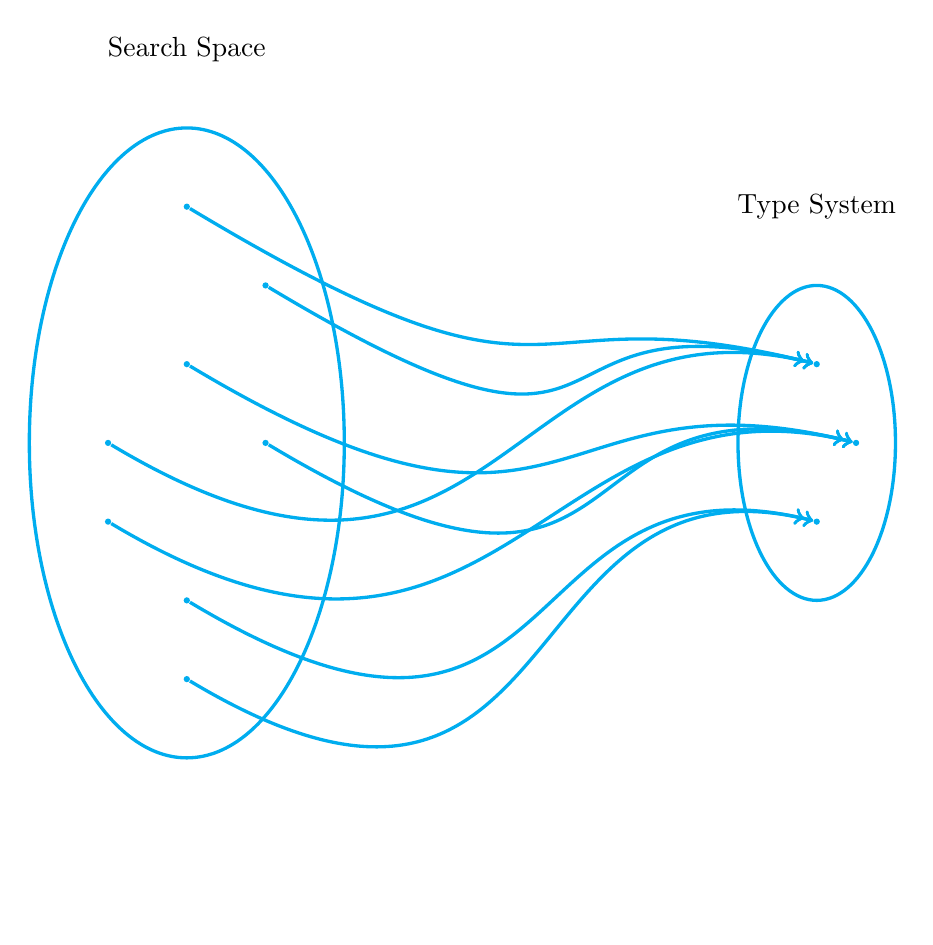
\begin{tikzpicture}

% -- center, xdim, ydim
\draw[very thick,cyan] \boundellipse{-2,0}{2}{4};
\draw[very thick,cyan] \boundellipse{6,0}{1}{2};
	
  % First, define nodes
% -- points F  
  
  \draw (-2,3) node[circle, inner sep=0.8pt, fill=cyan, label={{}}] (E) {};  
  \draw (6,1) node[circle, inner sep=0.8pt, fill=cyan, label={{}}] (F) {}; 

  \draw[very thick,cyan, ->>]  (E) .. controls +(5,-3) and +(-4,1).. (F);
  \path  ($(E)+(0,0.2)$) .. controls +(5,-3) and +(-4,1)..  ($(F)+(0,0.2)$) 
     {\foreach \i in {1,...,40} {  coordinate[pos=0.15+0.75*\i/40] (p\i) } };

  \draw (-1,2) node[circle, inner sep=0.8pt, fill=cyan, label={{}}] (A) {};
  \draw[very thick,cyan, ->>]  (A) .. controls +(5,-3) and +(-4,1).. (F);
  \path  ($(A)+(0,0.2)$) .. controls +(5,-3) and +(-4,1)..  ($(F)+(0,0.2)$) 
     {\foreach \i in {1,...,40} {  coordinate[pos=0.15+0.75*\i/40] (p\i) } };
	
  \draw (-3,0) node[circle, inner sep=0.8pt, fill=cyan, label={{}}] (B) {};
  \draw[very thick,cyan, ->>]  (B) .. controls +(5,-3) and +(-4,1).. (F);
  \path  ($(B)+(0,0.2)$) .. controls +(5,-3) and +(-4,1)..  ($(F)+(0,0.2)$) 
     {\foreach \i in {1,...,40} {  coordinate[pos=0.15+0.75*\i/40] (p\i) } };
	
% -- points in G

  \draw (-2,1) node[circle, inner sep=0.8pt, fill=cyan, label={{}}] (C) {};
  \draw (6.5,0) node[circle, inner sep=0.8pt, fill=cyan, label={{}}] (G) {};
  \draw[very thick,cyan, ->>]  (C) .. controls +(5,-3) and +(-4,1).. (G);
  \path  ($(C)+(0,0.2)$) .. controls +(5,-3) and +(-4,1)..  ($(G)+(0,0.2)$) 
     {\foreach \i in {1,...,40} {  coordinate[pos=0.15+0.75*\i/40] (p\i) } };	

\draw (-1,0) node[circle, inner sep=0.8pt, fill=cyan, label={{}}] (D) {};	
\draw[very thick,cyan, ->>]  (D) .. controls +(5,-3) and +(-4,1).. (G);
  \path  ($(C)+(0,0.2)$) .. controls +(5,-3) and +(-4,1)..  ($(G)+(0,0.2)$) 
     {\foreach \i in {1,...,40} {  coordinate[pos=0.15+0.75*\i/40] (p\i) } };	

\draw (-3,-1) node[circle, inner sep=0.8pt, fill=cyan, label={{}}] (H) {};	
\draw[very thick,cyan, ->>]  (H) .. controls +(5,-3) and +(-4,1).. (G);
  \path  ($(C)+(0,0.2)$) .. controls +(5,-3) and +(-4,1)..  ($(G)+(0,0.2)$) 
     {\foreach \i in {1,...,40} {  coordinate[pos=0.15+0.75*\i/40] (p\i) } };
	
% -- X
\draw (-2,-2) node[circle, inner sep=0.8pt, fill=cyan, label={{}}] (J) {};
  \draw (6,-1) node[circle, inner sep=0.8pt, fill=cyan, label={{}}] (X) {};
  \draw[very thick,cyan, ->>]  (J) .. controls +(5,-3) and +(-4,1).. (X);
  \path  ($(C)+(0,0.2)$) .. controls +(5,-3) and +(-4,1)..  ($(G)+(0,0.2)$) 
     {\foreach \i in {1,...,40} {  coordinate[pos=0.15+0.75*\i/40] (p\i) } };

\draw (-2,-3) node[circle, inner sep=0.8pt, fill=cyan, label={{}}] (K) {};
\draw[very thick,cyan, ->>]  (K) .. controls +(5,-3) and +(-4,1).. (X);
  \path  ($(C)+(0,0.2)$) .. controls +(5,-3) and +(-4,1)..  ($(G)+(0,0.2)$) 
     {\foreach \i in {1,...,40} {  coordinate[pos=0.15+0.75*\i/40] (p\i) } };

$\node [xshift=1cm,yshift=2cm] (A) at (-3,3) {Search Space};$

$\node [xshift=1cm,yshift=2cm] (A) at (5,1) {Type System};$
	
\end{tikzpicture}
\caption{Type system and the search space representation.} \label{fig:ss_ts}
\end{figure}

\subsection{Type System}
The \textit{Type System} is a partition of the states in the state space. It is calculated based of any property of each node in the search tree. \cite{Lelis2013CC}

A common misconception is think of \textit{type system} as state$-$space abstractions. \cite{Prieditis93} defines a state$-$space abstraction as a simplified version of the problem in which:
\begin{itemize}
\item The cost of the least$-$cost path between two abstracted states must less than or equal to the cost of the least$-$cost path between the corresponding two states in the original state$-$space.
\item Goal states in the original state$-$space must be goal states in the abstracted state$-$space.
\end{itemize}

In contrast with state$-$space abstractions, a \textit{type system} does not have these two requeriments. A \textit{type system} is just a partition of the nodes in the search tree.

The \textit{type system} can not be represented as a graph since \textit{type system} does not necessarily define relation between the types.

The relation between \textit{type system} and abstractions is the following: The \textit{type system} can not necessarily be used as abstractions, abstractions can always be used as \textit{type system}.

\subsection{Search Space and Search Tree}
\cite{lelis2013predicting} defines the search space and search tree in the following way: Let the \textit{underlying search tree} (\textit{UST}) be the full brute$-$force tree created from a connected, undirected and implicitely defined \textit{underlying search graph} (\textit{USG}) describing a state space. Some search algorithms expand a subtree of the \textit{UST} while searching for a solution (\textsf{e.g.,} a portion of the \textit{UST} might not be expanded due to heuristic guidance); we call this subtree the \textit{expanded search tree} \textit{(EST)}.\\

Let $G = (N,E)$ be a graph representing an \textit{ESG} where $N$ is its set of states and for each $n \in N op(n) = {op_{i}|(n, n_i) \in E}$ is its set of operators.

\theoremstyle{definition}
\begin{definition}{Type System}
Let S = (N,E) be a UST. $T = \{t_{1},...,t_{n} \}$ is a type system for S if it is a disjoint partitioning of N. If $n \in N$ and $t \in T$ with $n \in t$, we write $T(n) = t$.
\end{definition}

\texttt{SS} is a general method for approximating any function of the form $\varphi = \sum_{n \in S}z(n)$, where $z$ is any function assigning a numerical value to a node.  $\varphi$ represents a numerical property of the search tree rooted at $n\sp{*}$. For instance, if $z(n)=1$ for all $n \in S$, then $\varphi$ is the size of the tree.\\

Instead of traversing the entire tree and summing all $z-$values, \texttt{SS} assumes subtrees rooted at nodes of the same type will have equal values of $\varphi$ and so only one node of each type, chosen randomly, is expanded. This is the key to $\texttt{SS}$'s efficiency since the search trees of practical interest have far too many nodes to be examined examined exhaustively.\\

Given a search tree $S$ and a type system $T$, \texttt{SS} estimates $\varphi$ as follows. First, it samples the tree and returns a set $A$ of $representative-weight$ pairs, with one such pair for every unique type seen during sampling. In the pair $\left\langle s,w \right\rangle$ in $A$ for type $t \in T$, $n$ is the unique node of type $t$ that was expanded during search and $w$ is an estimate of the number of nodes type $t$ in the tree. $\varphi$ is then approximated by $\hat{\varphi}$, defined as, $\hat{\varphi} =  \sum_{\left\langle s,w \right\rangle \in A}w \times z(n)$.\\

By making $z(n) = 1$ for all $n \in S$ \texttt{SS} prooduces an estimate $\hat{J}$ of $J$. Similarly to our approach with \texttt{CS}, we obtain $\hat{T}$ by multiplying $\hat{J}$ by the heuristic evaluation time.


\begin{algorithm}
\SetKwInOut{Input}{Input}
\SetKwInOut{Output}{Output}
\Input{root $n\sp{*}$ of a tree and a type system $T$}
\Output{an array of sets $A$, where $A[i]$ is the set of pairs $<n,w>$ for the nodes $n$ expanded at level $i$.}

$A[0] \leftarrow \{\left\langle  n\sp{*},1 \right\rangle \}$

$i \leftarrow 0$

\While{A[i] is not empty} {
	\For{each element $\left\langle n,w \right\rangle$ in $A[i]$} {
		\For{each child $\hat{n}$ of n} {
			\If{$g(\hat{n}) + h(\hat{n}) \leq d$} {
				\If{$A[i+1]$ contains an element $\left\langle n\sp{'}, w\sp{'} \right\rangle$ with $T(n\sp{'}) = T(\hat{n})$} {
				$w\sp{'} \leftarrow w\sp{'} + w$\\ 
				with probability $w/w\sp{'}$, replace $\left\langle n\sp{'}, w\sp{'} \right\rangle$ in\\ $A[i+1]$ by $\left\langle \hat{n},w\sp{'} \right\rangle$
				} \Else {	
					insert new element $\left\langle \hat{n},w\sp{'} \right\rangle$	 in $A[i+1]$
				}
			}
		}
	}
	$i \leftarrow i + 1$
}
\caption{SS, a single probe}
\label{alg:ss_algorithm}
\end{algorithm}

In \texttt{SS} the types are required to be partially ordered: a node's type must be strictly greater than the type of its parent. This can be guaranteed by adding the depth of a node to the type system and then sorting the types lexicographically. That is why in our implementation of \texttt{SS} types at one level are treated separately from types ate another level by the division of $A$ into groups $A[i]$, where $A[i]$ is the set of representative$-$weight pairs for the types encountered at level $i$. If the same type occurs on differente levels the occurrences will be treated as if they were different types $-$ the depth of search is implicitly included into all of our type systems.\\

Algorithm \ref{alg:ss_algorithm} shows \texttt{SS} in detail. Representative nodes from $A[i]$ are expanded to get representative nodes for $A[i+1]$ as follows. $A[0]$ is initialized to contain only the root of the search tree to be probed, with weight 1 (Line 1). In each iteration (Lines 4 through 11), all nodes in $A[i]$ are expanded. The children of each node in $A[i]$ are considered for inclusion in $A[i+1]$ if their $f-$value do not exceed an upper bound $d$ provided as input to \texttt{SS}. If a child $\hat{n}$ has a type $t$ that is already represented in $A[i+1]$ by another node $n\sp{'}$, then a $merge$ action on $\hat{n}$ and $n\sp{'}$ is performed. In a merge action we increase the weight in the corresponding representative$-$weight pair of type $t$ by the weight $w(n)$ of $\hat{n}$'s parent $n$ (from level $i$) since there were $w(n)$ nodes at level $i$ that are assumed to have children of type $t$ at level $i+1$. $\hat{n}$ will replace $n\sp{'}$ according to the probability shown in Line 9. \cite{chen1992heuristic} proved that this probability reduces the variance of the estimation. Once all the states in $A[i]$ are expanded, we move to the next iteration.\\

One run of the \texttt{SS} algorithm is called a $probe$. \cite{chen1992heuristic} proved that the expected value of $\hat{\varphi}$ converges to $\varphi$ in the limit as the number of probes goes to infinity. As \cite{lelis2014estimating}, \texttt{SS} is not able to detect duplicated nodes in its sampling process. As a result, since A$\sp{*}$ does not expanded duplicates, \texttt{SS} usually overestimates the actual number of nodes A$\sp{*}$ expands. Thus, in the limit, as the number of probes grows large, \texttt{SS}'s prediction converges to a number which  is likely to overestimate the A$\sp{*}$ search tree size. We test empirically whether \texttt{SS} is able to allow \texttt{RGHS} to make good subset selects despite being unable to detect duplicated nodes during sampling.\\

Similarly to \texttt{CS}, we also define a time$-$limit to run \texttt{SS}. We use \texttt{SS} with an iterative$-$deepening approach in order to ensure an estimate of $\hat{J}$ and $\hat{T}$ before reaching the time limit. We set the upper bound $d$ to the heuristic value of the start state and, after performing $p$ probes, if there is still time, we increase $d$ to twice its previous value. The values of $\hat{J}$ and $\hat{T}$ is given by the prediction produced for the last $d-$value in which \texttt{SS} was able to perform all $p$ probes.\\

\texttt{SS} must also be able to estimate the values of $\hat{J}(\zeta\sp{'})$ and $\hat{T}(\zeta\sp{'})$ for any subset $\zeta\sp{'}$ of $\zeta$. This is achieved by using \texttt{SS} to estimate b$-$culprits (See Definition \ref{def:def_bculprits}) instead of the search tree size directly. Similarly to \texttt{CS, SS} used $h_{min}$ of the heuristics in $\zeta$ to decide when to prune a node (See Line 6 \ref{alg:ss_algorithm}) while sampling. This ensures that \texttt{SS} expands a node $n$ if A$\sp{*}$ employing at least one of the heuristics in $\zeta$ would expand $n$ according to bound $d$. The $C_{B}$ counter of each b$-$culprit $B$ encountered during $SS$'s probe is given by,

\begin{equation}
C_{B} = \sum_{\left\langle n,w \right\rangle \in A \wedge B(n) = B}w
\label{eq:eq_CB}
\end{equation}

We recall that to compute $B(n)$ for node $n$ one needs to define a bound $b$. Here we use the bound $d$ used by \texttt{SS}. The average value of $C_{B}$ across $p$ probes is used to predict the search tree size for a given subset $\zeta\sp{'}$. As explained for \texttt{CS}, this can be done by traversing over all b$-$culprits once.\\

\section{8-tile-puzzle Case Using type system}
\noindent
In this thesis we use \textit{type system} based only in heuristics.\cite{zahavi2010predicting} use the simpliest heuristic$-$based \textit{type system} in which two nodes $n$ and $n\sp{'}$ are of the same type if they have the same heuristic value. \\

\begin{figure}[htb]
\centering
\begin{forest}
 [\usebox\myboxc \hspace*{1.4in} \usebox\myboxb]
\end{forest}
\caption{The heuristic value is the position of the empty tile in a Specific state.} \label{fig:type_system}
\end{figure}

Let's explain how \textit{type system} works through an example. The problem of 8$-$tile$-$puzzle in the Figure \ref{fig:type_system}, the center tile is labeled with the letter \texttt{M}, the corners labeled with \texttt{C} and the mediums with \texttt{E}. For this problem, we can define the \textit{type system} based on the position of the empty tile regarding the position of the empty tile in the goal state. For this case, two nodes $n$ and $n\sp{'}$ would be of the same type if $n$ and $n\sp{'}$ have the empty tile with the same letter and with the same distance to the empty tile of the goal state.\\

In the Figure \ref{fig:empty_space_ts}, each row represent a type. The first board shows the empty tile in the center with distance to the empty tile in the goal state equal to 2. The shortest path to get to the empty tile in the goal state would be doing: down$-$left or right$-$down. Which both moves represent the same cost. Then, the type would be (2,\texttt{M}). In the next board, the empty tile is in the left top, and use the letter \texttt{C}. The minimum distance is 4 because to get the goal empty tile is necessary to do: down$-$down$-$right$-$right or right$-$right$-$down$-$down, etc. So the type would be (4, \texttt{C}). In the next board, there are two tiles that have the same type, because both have the same letter \texttt{M} with distance equal to 3. Then, both have the type (3,E). The fourth row have two boards with the same type, because both have the same letter \texttt{C} with distance equal to 2. Then, both have the type (2, \texttt{C}). The fifth row have two boards with the same type, because both have the same letter \texttt{E} with distance equal to 1. Then, both have the type (1, \texttt{E}). In the last row the empty tile is in the goal empty tile. So, the distance is zero and the letter is \texttt{C}. The type would be (0, \texttt{C}).

% print types
\begin{figure}[htb]
\centering
\begin{forest}
 [\usebox\myboxcenter]
 $\node [xshift=1cm,yshift=2cm] (A) at (2,0) {(2, M)};$
\end{forest}

\begin{forest}
 [\usebox\myboxcornerone]
 $\node [xshift=1cm,yshift=2cm] (A) at (2,0) {(4, C)};$
\end{forest}

\begin{forest}
 [\usebox\myboxmediumleft \hspace*{0.2in} \usebox\myboxmediumup]
 $\node [xshift=1cm,yshift=2cm] (A) at (4,0) {(3, E)};$
\end{forest}

\begin{forest}
 [\usebox\myboxcornerthree \hspace*{0.2in} \usebox\myboxcornertwo]
 $\node [xshift=1cm,yshift=2cm] (A) at (4,0) {(2, C)};$
\end{forest}

\begin{forest}
 [\usebox\myboxmediumdown \hspace*{0.2in} \usebox\myboxmediumright]
 $\node [xshift=1cm,yshift=2cm] (A) at (4,0) {(1, E)};$
\end{forest}

\begin{forest}
 [\usebox\myboxcornerfour]
 $\node [xshift=1cm,yshift=2cm] (A) at (2,0) {(0, C)};$
\end{forest}
\caption{Each row has one or two states that represent the same type.} \label{fig:empty_space_ts}
\end{figure}

\section{SS step by step}
\noindent
% -- Explaining Stratified Sampling
In the Figure \ref{fig:ts_search_tree}, we can see how \textit{Type System} works. In the Level 1, we have the root node, the $w$ initialized with one. Let's suppose that three nodes are generated by the root node in the Level 2. The nodes in the Level 2 have the following types: red, blue and red from left to right respectively, and each node recive the same $w$ of the father. In the Level 2 we apply \texttt{SS}'s assumption, two nodes in the same level that have the same type (The same color) root subtrees of the same size and so only one node of each type must be chosen randomly to be expanded. There are two nodes with type red in Level 2. In that way, we choose randomly one of them. Let's suppose we choose the right red node. Then, we have to update the number of nodes with the type red using the $w$, both red node types have $w=1$, then we sum the $w$ and the new $w=2$. As a result, in the Level 2 we will have two nodes of red type and one node with blue type. \\

\begin{figure}[htb]
\centering
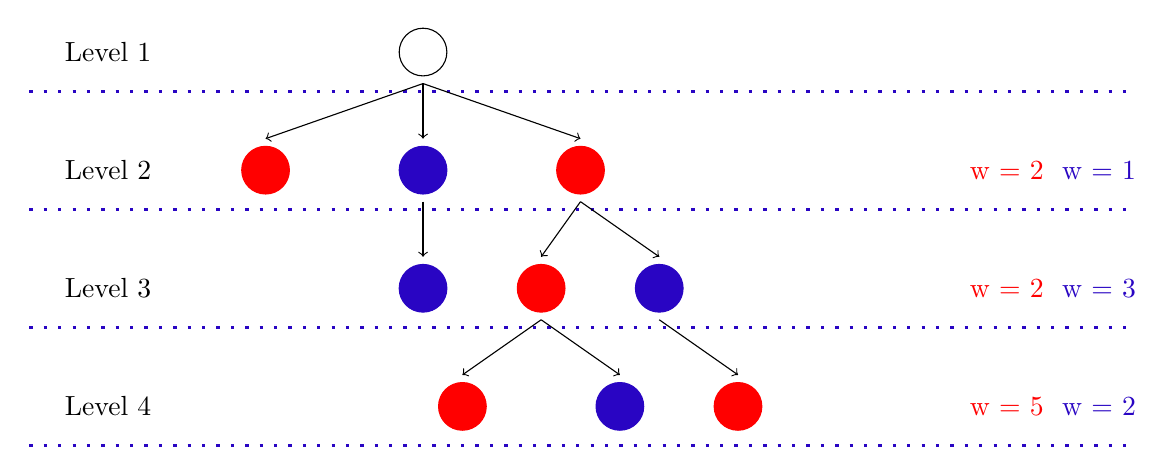
\begin{tikzpicture}

\draw[very thick,blue,loosely dotted] (-2,0) -- (12,0);
\draw[very thick,blue,loosely dotted] (-2,-1.5) -- (12,-1.5);
\draw[very thick,blue,loosely dotted] (-2,-3) -- (12,-3);
\draw[very thick,blue,loosely dotted] (-2,-4.5) -- (12,-4.5);

\node [xshift=1cm,yshift=2cm] (A) at (-2,-1.5) {Level 1};
\node [xshift=1cm,yshift=2cm] (A) at (-2,-3) {Level 2};
\node [xshift=1cm,yshift=2cm] (A) at (-2,-4.5) {Level 3};
\node [xshift=1cm,yshift=2cm] (A) at (-2,-6) {Level 4};

% -- level 1
\draw[black,fill=white] (3,0.5) circle (2ex);

% -- level 2
\draw[red,fill=red] (1,-1) circle (2ex);
\draw[blue,fill=blue] (3,-1) circle (2ex);
\draw[red,fill=red] (5,-1) circle (2ex);

% -- level 3
\draw[blue,fill=blue] (3,-2.5) circle (2ex);
\draw[red,fill=red] (4.5,-2.5) circle (2ex);
\draw[blue,fill=blue] (6,-2.5) circle (2ex);

% -- level 4
\draw[red,fill=red] (3.5,-4) circle (2ex);
\draw[blue,fill=blue] (5.5,-4) circle (2ex);
\draw[red,fill=red] (7,-4) circle (2ex);

% -- draw arrows
\draw[->] (3,0.1) -- (1,-0.6);
\draw[->] (3,0.1) -- (3,-0.6);
\draw[->] (3,0.1) -- (5,-0.6);

\draw[->] (3,-1.4) -- (3,-2.1);

\draw[->] (5,-1.4) -- (4.5,-2.1);
\draw[->] (5,-1.4) -- (6,-2.1);

\draw[->] (4.5,-2.9) -- (3.5,-3.6);
\draw[->] (4.5,-2.9) -- (5.5,-3.6);

\draw[->] (6,-2.9) -- (7,-3.6);

\node [xshift=1cm,yshift=2cm] (A) at (10,-3) {\textcolor{red}{w = 2 } \textcolor{blue}{w = 1}};
\node [xshift=1cm,yshift=2cm] (A) at (10,-4.5) {\textcolor{red}{w = 2 } \textcolor{blue}{w = 3}};
\node [xshift=1cm,yshift=2cm] (A) at (10,-6) {\textcolor{red}{w = 5 } \textcolor{blue}{w = 2}};
\end{tikzpicture}
\caption{Search tree using Type System} \label{fig:ts_search_tree}
\end{figure}

When nodes in the Level 2 are expanded. The blue node expands one node of type blue and the red node expands two nodes of type red and blue. The question here is how many nodes would be generated in the Level 3? The answer is: $1 \times \textcolor{blue}{blue} + 2 \times \textcolor{red}{red} + 2 \times \textcolor{blue}{blue}$. So, in the Level 3 we will have 2 nodes of red type and 3 nodes of type blue.\\ 

In the Level 3 the $w$ of the node blue would have the same $w$ of the father. The father has $w = 1$, then the child has $w = 1$. The $w$ of the red type and blue type would be 2. Once the $w$ has been updated for each node in the Level 3 we apply the \texttt{SS}'s assumption again. There are two nodes with type blue. So, we choose randomly one of them and update their $w$. Let's choose the right blue type and the updated $w$ would be 3 because 1 from the left blue type plus the 2 from the right blue type.\\

When nodes in the Level 3 are expanded. They are expanded in the following way: The red node expands two nodes of types red and blue and the blue node expands one of red type. How many nodes would be generated at Level 4, then? The answer is: $2 \times \textcolor{red}{red} + 3 \times \textcolor{red}{red} + 2 \times \textcolor{blue}{blue}$. Therefore, in the Level 4, we will have five nodes of type red and two nodes of type blue.\\

Finally, the number of nodes expanded in the search tree is obtained summing all $w$ plus one (The root node). As a result, the number of nodes expanded in the search tree would be $ 15 + 1 = 16$.\\

\section{Comparison between SS and IDA*}
\noindent
\texttt{SS} is an algorithm that estimates the number of nodes expanded performed by heuristic search algorithm seeking solutions in state space. We apply \texttt{SS} to predict the number of nodes expanded by IDA$\sp{*}$ in a given $f-$layer when using a consistent heuristics.\\

We first ran IDA$\sp{*}$ for Fast$-$Downward benchmark for optimal domains. Our evaluation metric is coverage, \texttt{i.e.,} number of problems solved within 30 minutes time limit. We note that in 30 minutes non all the instances for a specific domain using a consistent heuristic can be solved. Afterwards, run \texttt{SS} using as a threshold the $f-$layer for each instance of each domain, this process is executed using different number of probes \texttt{i.e.,} 1, 10, 100, 1000 and 5000.\\

\begin{equation}
\frac{\sum_{s\in PI} \frac{Pred(s, d) - R(s, d)}{R(s, d)}}{|PI|}
\label{eq:eq_comparison}
\end{equation}

Where $PI$ is the set of problem instances, $Pred(s,d)$ and $R(s,d)$ are the predicted and actual number of nodes expanded by IDA$\sp{*}$ for start state $s$ and cost bound $d$. A perfect score according to the measure is $0.00$.\\

The Table \ref{tb:comparison} shows how the relative$-$error behavies when \texttt{SS} makes prediction of the number of nodes expanded by IDA$\sp{*}$ when it is searching with a specific heuristic and cost thresold. The heuristic used in this experiment is $hmax$. Five probes were used: 1, 10, 100, 1000 and 5000. The average value of IDA$\sp{*}$ and time were used. The relative$-$error gets a perfect score while increasing the number of probes. For Barman, the relative$-$error goes from $0.60$ for 1 probe to $0.45$ for 10 probes, $0.20$ for 100 probes, $0.07$ for 1000 probes and $0.04$ for 5000 probes. In the case of time, while the number of probes increase, \texttt{SS} need to spend more time calculating the size of the search tree. Then, the time increase. For Barman, the time goes from $0.06\ seconds$ for 1 probe to $0.32\ seconds$ for 10 probes, $3.21\ seconds$ for 100 probes, $32.57\ seconds$ for 1000 probes and $214.59\ seconds$ for 5000 probes. There are domains such as: Parcprinter, Parking, Pegsol and Visitall that have perfect score using 5000 probes. In the case of Tidybot, the relative$-$error using 1 probe is smaller than using 10 probes. The reason might be the search tree generated for some instances or the stochastic behavior of \texttt{SS} that sometimes it will choose a node that expand a search tree that will be more expensive to expand. The last column \textsf{n} represent the number of instances where IDA$\sp{*}$ found the number of nodes expanded when it is searching with $hmax$ and cost threshold. The 2011 \texttt{IPC} domains contains 20 instances per domain. Floortile only have 2 instances, it means that when running IDA$\sp{*}$ for all the instances of Floortile only two instances (opt$-$p01$-$001.pddl and opt$-$p03$-$006.pddl) have found number of nodes expanded under some threshold. In summary, we proved that for 2011 \texttt{IPC} domains, \texttt{SS} estimations converges to the real search tree size generated by IDA$\sp{*}$ when the number of probes goes to infinity.

% Please add the following required packages to your document preamble:
% \usepackage{multirow}
\begin{table}[]
\footnotesize\setlength{\tabcolsep}{1.2pt}
\centering
\caption{Comparison between \texttt{SS} and IDA$\sp{*}$ for 1, 10, 100, 1000 and 5000 probes using $hmax$ heuristic.}
\label{tb:comparison}
\begin{tabular}{lccccccccccccc}
\hline
\multirow{3}{*}{Domain} & \multicolumn{13}{c}{$hmax$}                                                                                                                     \\ \cline{2-14} 
                        & \multirow{2}{*}{IDA$\sp{*}$} & \multirow{2}{*}{time} & \multicolumn{5}{c}{relative$-$error} & \multicolumn{5}{c}{time}   & \multirow{2}{*}{n} \\ \cline{4-13}
                        &                              &                       & 1   & 10   & 100   & 1000   & 5000   & 1 & 10 & 100 & 1000 & 5000 &                    \\ \hline
Barman & 8835990.00& 6016.38& 0.60& 0.45& 0.20& 0.07& 0.04& 0.06& 0.32& 3.21& 32.57& 214.59& 20\\
Elevators & 1012570.00& 4987.57& 0.84& 0.42& 0.23& 0.13& 0.10& 1.40& 9.85& 96.37& 994.33& 4425.93& 20\\
Floortile & 30522300.00& 3919.72& 2.02& 0.62& 0.40& 0.14& 0.11& 0.01& 0.07& 0.69& 6.93& 36.60& 2\\
Nomystery & 6565740.00& 3256.86& 0.53& 0.26& 0.07& 0.03& 0.01& 0.07& 0.38& 3.63& 36.35& 181.03& 20\\
Openstacks & 80108.50& 4017.19& 0.03& 0.03& 0.03& 0.03& 0.03& 94.79& 774.86& 1067.84& 10929.00& 11174.30& 20\\
Parcprinter & 1.00& 0.00& 0.00& 0.00& 0.00& 0.00& 0.00& 0.01& 0.04& 0.35& 3.48& 17.29& 20\\
Parking & 374925.00& 5607.50& 0.17& 0.04& 0.01& 0.00& 0.00& 1.79& 11.36& 114.28& 1196.83& 5835.03& 20\\
Pegsol & 68763.70& 5.00& 0.17& 0.04& 0.02& 0.01& 0.00& 0.01& 0.04& 0.37& 3.69& 17.88& 20\\
Scanalyzer & 8449890.00& 4920.58& 0.43& 0.25& 18.63& 0.02& 0.01& 3.13& 28.79& 273.74& 3033.06& 10254.00& 20\\
Sokoban & 3118530.00& 3932.69& 0.41& 0.26& 0.11& 0.05& 0.04& 0.31& 2.00& 21.42& 222.47& 1056.61& 20\\
Tidybot & 444473.00& 5632.08& 300.86& 1072.40& 5.88& 0.01& 0.01& 4.40& 26.48& 238.76& 2747.10& 11925.40& 20\\
Transport & 2622880.00& 2253.51& 0.63& 0.54& 0.24& 0.15& 0.11& 0.09& 0.61& 5.89& 59.37& 290.31& 20\\
Visitall & 71032400.00& 3704.78& 0.12& 0.04& 0.01& 0.00& 0.00& 0.00& 0.05& 0.56& 5.77& 28.07& 20\\
Woodworking & 5139070.00& 4944.76& 1.28& 0.69& 0.27& 0.17& 0.07& 0.15& 1.33& 13.21& 130.82& 664.08& 20\\ \hline
\end{tabular}
\end{table}

\section{Comparison between SS and A*}
\noindent
The Table \ref{tb:ipdb_lmcut_mands} shows that \texttt{SS} is not a good predictor for A$\sp{*}$ and that is because \texttt{SS} does not count for duplicate nodes and A$\sp{*}$ does. \texttt{SS} overestimate the A$\sp{*}$ search tree size. As a result, \texttt{SS} often overestimates by several orders of magnitude the actual A$\sp{*}$ search tree.\\

Three heuristics were used: ipdb, \texttt{LM-Cut} and M$\&$S.  The last column \textsf{n} represent the number of instances solved by A$\sp{*}$ using the three heuristics. For this experiment we decided to use only the instances that are solved by the three heuristics at the same time. The columns with A$\sp{*}$ represents the average of number of nodes expanded by A$\sp{*}$ using a specific heuristic. The column with \texttt{SS}$-$error represents the relative$-$error formula \ref{eq:eq_comparison}.\\

For Barman: Using M$\&$S, A$\sp{*}$ expands in average 6.67e$+$06 which is less nodes than ipdb$-$1.72e$+$07 and \texttt{LM-Cut}$-$7.45e$+$06. However, using M$\&$S, \texttt{SS}$-$error is 1.26e$+$36, ipdb$-$8.68e$+$31 and \texttt{LM-Cut}$-$2.21e$+$30. Which indicates that the number of nodes expanded by \texttt{SS} in average is in the order of magnitude of 30 to 40. In Visitall, \texttt{SS}$-$error shows that \texttt{SS} overestimates A$\sp{*}$ highly, which represent a very bad prediction of \texttt{SS}. In Openstack: Using the three heuristics, A$\sp{*}$ expands almost the same number of nodes for the 4 instances solved. And \texttt{SS}$-$error shows a score near to the perfect and the reason is because \texttt{SS} expands less nodes than A$\sp{*}$. 



% Please add the following required packages to your document preamble:
% \usepackage{multirow}
\begin{table}[]
\footnotesize\setlength{\tabcolsep}{1.2pt}
\centering
\caption{Poor prediction of SS against A* using ipdb, \texttt{LM-Cut} and M$\&$S with 500 probes}
\label{tb:ipdb_lmcut_mands}
\begin{tabular}{lC{2cm}C{2cm}C{2cm}C{2cm}C{2cm}C{2cm}C{2cm}}
\hline
\multirow{2}{*}{Domain} & \multicolumn{2}{c}{ipdb} & \multicolumn{2}{c}{\texttt{LM-Cut}} & \multicolumn{2}{c}{M$\&$S} & \multirow{2}{*}{n} \\ \cline{2-7}
                     & A*          & SS$-$error         & A*                & SS$-$error                & A*           & SS$-$error          &                    \\ \hline
Barman               & 1.72e+07    & 8.68e+31   & 7.45e+06          & 2.21e+30          & 6.67e+06     & 1.26e+36    & 4                  \\
Floortile            & 1.40e+07    & 1.74e+18   & 702435            & 4.68e+14          & 4.46e+06     & 1.90e+12    & 4                  \\
Nomystery            & 40169.7     & 6.71e+32   & 267100            & 6.14e+19          & 8236         & 1.20e+20    & 9                  \\
Openstacks           & 570099      & 0.61884    & 570099            & 0.677425          & 569984       & 0.672143    & 4                  \\
Parcprinter          & 1157        & 2.56e+22   & 1363.67           & 2.33e+21          & 766.333      & 6.36e+20    & 3                  \\
Pegsol               & 841693      & 2901.39    & 398221            & 6859.86           & 933430       & 779.017     & 16                 \\
Scanalyzer           & 337894      & 3.94e+33   & 334747            & 7.58e+31          & 337833       & 2.42e+31    & 3                  \\
Sokoban              & 376755      & 1.04e+07   & 45374             & 2.74e+06          & 739775       & 5.60e+08    & 9                  \\
Transport            & 1.89e+06    & 2.91e+38   & 1.49e+06          & 1.15e+25          & 1.73e+06     & 1.50e+29    & 2                  \\
Visitall             & 253710      & 1.69e+46   & 253195            & 1.69e+46          & 253521       & 1.71e+46    & 8                  \\
Woodworking          & 3.21e+06    & 2.53e+18   & 3.20e+06          & 2.76e+18          & 3.21e+06     & 2.48e+18    & 3                  \\ \hline
\end{tabular}
\end{table}

\section{Approximation Analysis for SS and A*}
\noindent
In order to understand how \texttt{SS} and A$\sp{*}$ behaves we have created plots with the fixed range of 2 . This way we are going to have 4 different regions as shown in the Figure a. Points on regions 2 and 3 are heuristics that \texttt{SS} correctly chose to be used with A$\sp{*}$. Points following on the other regions are those choices \texttt{SS} made incorrectly.



\begin{figure}[!htb]
\minipage{0.32\textwidth}
  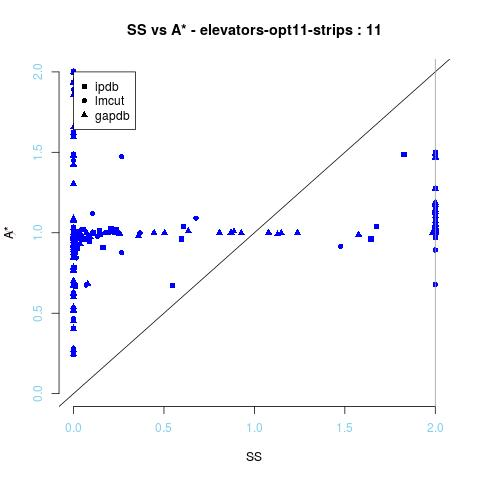
\includegraphics[width=\linewidth]{images/elevators-opt11-strips}
\endminipage\hfill
\minipage{0.32\textwidth}
  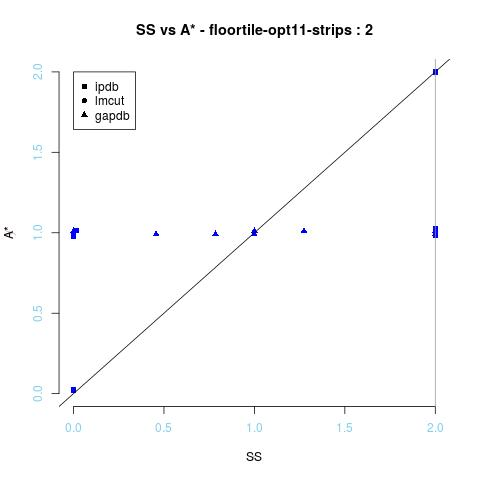
\includegraphics[width=\linewidth]{images/floortile-opt11-strips}
\endminipage\hfill
\minipage{0.32\textwidth}%
  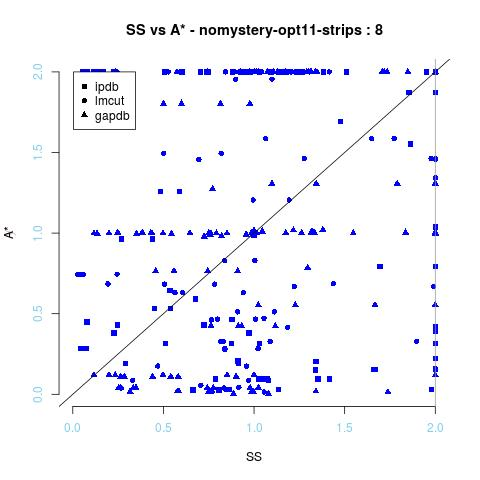
\includegraphics[width=\linewidth]{images/nomystery-opt11-strips}
\endminipage

%jump
\minipage{0.32\textwidth}
  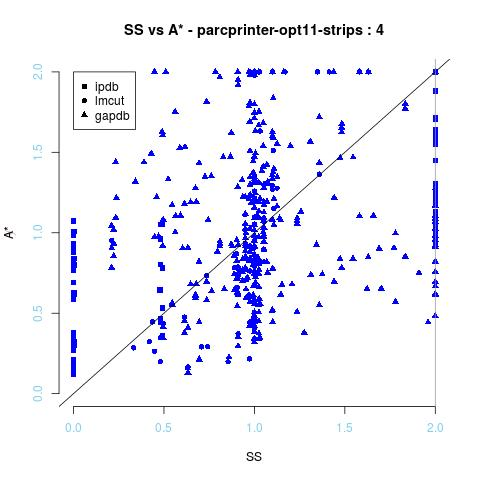
\includegraphics[width=\linewidth]{images/parcprinter-opt11-strips}
\endminipage\hfill
\minipage{0.32\textwidth}
  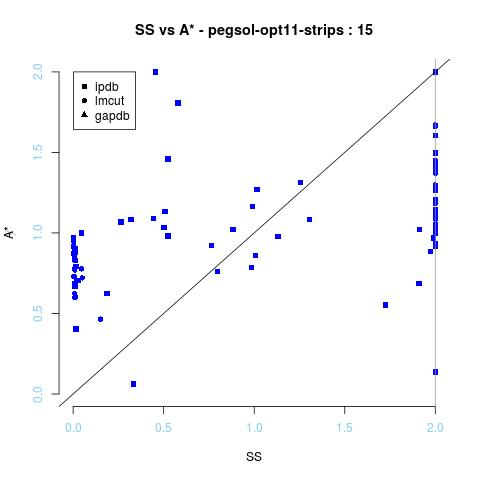
\includegraphics[width=\linewidth]{images/pegsol-opt11-strips}
\endminipage\hfill
\minipage{0.32\textwidth}
  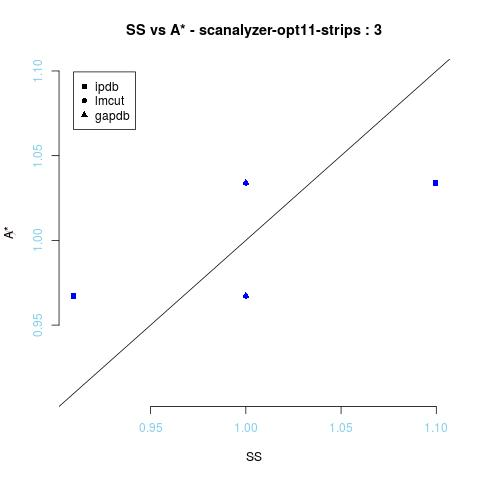
\includegraphics[width=\linewidth]{images/scanalyzer-opt11-strips}
\endminipage\hfill

%jump
\minipage{0.32\textwidth}
  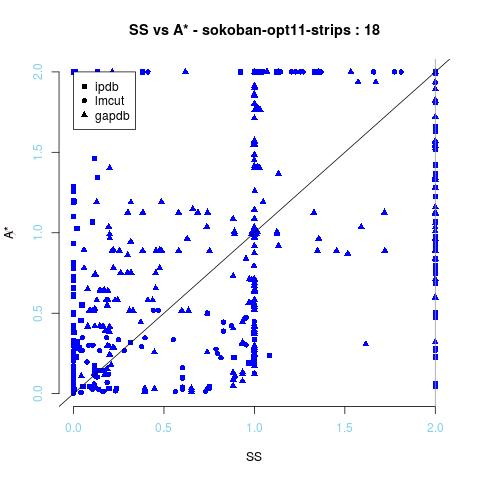
\includegraphics[width=\linewidth]{images/sokoban-opt11-strips}
\endminipage\hfill
\minipage{0.32\textwidth}
  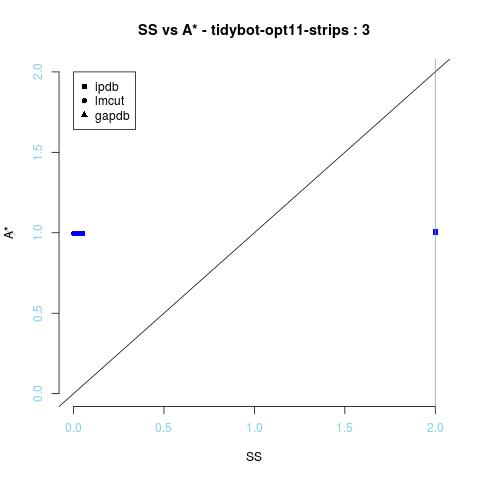
\includegraphics[width=\linewidth]{images/tidybot-opt11-strips}
\endminipage\hfill
\minipage{0.32\textwidth}
  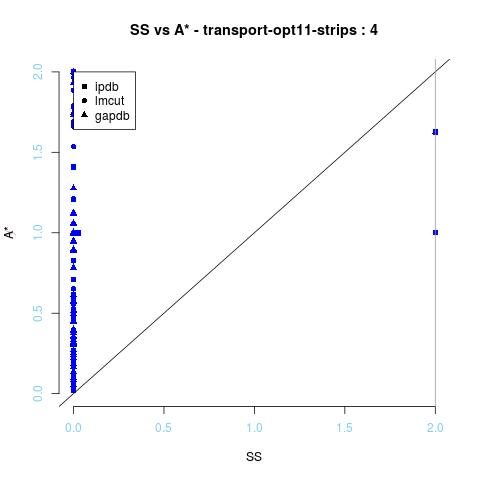
\includegraphics[width=\linewidth]{images/transport-opt11-strips} 
\endminipage\hfill

%jump
\minipage{0.32\textwidth}
  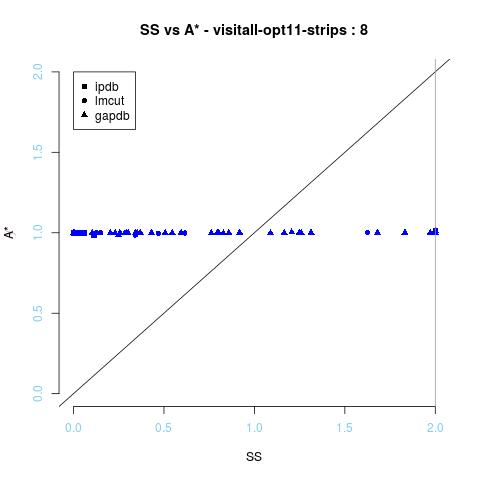
\includegraphics[width=\linewidth]{images/visitall-opt11-strips}
\endminipage\hfill
\minipage{0.32\textwidth}
  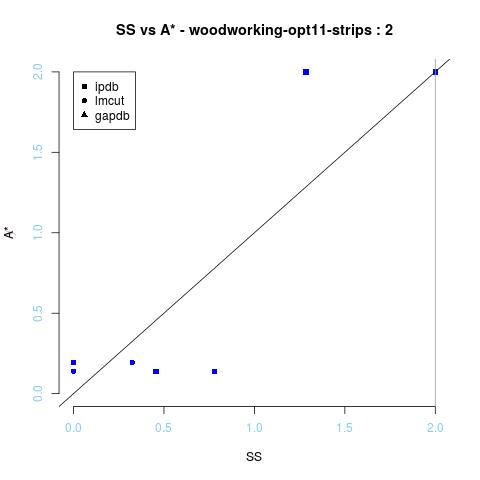
\includegraphics[width=\linewidth]{images/woodworking-opt11-strips}
\endminipage\hfill
\caption{\texttt{SS} vs A$\sp{*}$ for the optimal domains.}\label{fig:img_analysis_domains}
\end{figure}

\begin{table}[!htb]
\centering
\caption{My caption}
\label{my-label}
\begin{tabular}{lc}
\hline
Domain      & I and IV \\ \hline
Elevators   & 78.57    \\
Floortile   & 96.08    \\
Nomystery   & 71.82    \\
Parcprinter & 70.50    \\
Pegsol      & 96.83    \\
Scanalyzer  & 100.00   \\
Sokoban     & 89.31    \\
Tidybot     & 100.00   \\
Transport   & 51.78    \\
Visitall    & 98.05    \\
Woodworking & 100.00   \\ \hline
\end{tabular}
\end{table}



\clearpage
% ---

% PARTE
% ----------------------------------------------------------
\part{Empirical Evaluation}
% ----------------------------------------------------------
%% abtex2-modelo-include-comandos.tex, v-1.9.5 laurocesar
%% Copyright 2012-2015 by abnTeX2 group at http://www.abntex.net.br/ 
%%
%% This work may be distributed and/or modified under the
%% conditions of the LaTeX Project Public License, either version 1.3
%% of this license or (at your option) any later version.
%% The latest version of this license is in
%%   http://www.latex-project.org/lppl.txt
%% and version 1.3 or later is part of all distributions of LaTeX
%% version 2005/12/01 or later.
%%
%% This work has the LPPL maintenance status `maintained'.
%% 
%% The Current Maintainer of this work is the abnTeX2 team, led
%% by Lauro César Araujo. Further information are available on 
%% http://www.abntex.net.br/
%%
%% This work consists of the files abntex2-modelo-include-comandos.tex
%% and abntex2-modelo-img-marca.pdf
%%

% ---
% Este capítulo, utilizado por diferentes exemplos do abnTeX2, ilustra o uso de
% comandos do abnTeX2 e de LaTeX.
% ---

\externaldocument[I-]{chapter03}

\chapter{Empirical Evaluation}\label{ch:empirical_evaluation}
\noindent

\section{Comparison between SS and IDA*}
\noindent
\texttt{SS} was shown to produce good predictions of the IDA$\sp{*}$ search tree size (Lelis et al., \citeyear{lelis2013predicting}). Iterative-Deepening A$\sp{*}$ (IDA$\sp{*}$) is a heuristic search algorithm that uses cost function for looking the solution in the search space and in each iteration uses \texttt{DFS} to prune the branch until reaching the cost threshold (Korf, Reid and Edelkamp, \citeyear{korf2001timecomplexity}).
 
\texttt{SS} is able to produce good predictions for IDA$\sp{*}$ also in domain-independent planning, and we will show that it produces very inaccurate predictions for A$\sp{*}$

In this experiment \texttt{SS} estimates the search tree size generated by IDA$\sp{*}$ using a consistent heuristic. \texttt{SS} estimates the size of the search tree up to some defined $f$-layer in the tree.

We first run IDA$\sp{*}$ in domain-independent planning benchmark problems within 30 minutes time limit. Then we run \texttt{SS} limited by different $f$-layers encountered in the IDA$\sp{*}$ searches. We experiment with the following number of probes: 1, 10, 100, 1000 and 5000.

We use the \textit{relative unsigned error} (Lelis et al., \citeyear{lelis2012fast}), which we call relative-error, for short, to measure prediction accuracy. The relative-error is shown in Equation \ref{eq:eq_comparison} below.

\begin{equation}
\frac{\sum_{s\in PI} \frac{Pred(s, d) - R(s, d)}{R(s, d)}}{|PI|}
\label{eq:eq_comparison}
\end{equation}

\begin{itemize}
  \item $PI$ represent all the instances for a domain.
  \item $Pred(s,d)$ is the estimation of the search tree size expanded by IDA$\sp{*}$ for start state $s$ and cost bound $d$.
  \item $R(s,d)$ is the real number of nodes expanded by IDA$\sp{*}$ for start state $s$ and cost bound $d$.
\end{itemize}
A relative error of 0.0 means that SS was able to produce perfect predictions.

% Please add the following required packages to your document preamble:
% \usepackage{multirow}
\begin{table}[]
%\footnotesize\setlength{\tabcolsep}{1.2pt}
\tiny\setlength{\tabcolsep}{2pt}
\centering
\caption{Comparison between \texttt{SS} and IDA$\sp{*}$ for 1, 10, 100, 1000 and 5000 probes using $hmax$ heuristic.}
\label{tb:comparison}
\begin{tabular}{lrrrrrrrrrrrrr}
\hline
\multirow{3}{*}{Domain} & \multicolumn{13}{c}{$hmax$}                                                                                                                     \\ \cline{2-14} 
                        & \multirow{2}{*}{IDA$\sp{*}$} & \multirow{2}{*}{time} & \multicolumn{5}{c}{relative$-$error} & \multicolumn{5}{c}{time}   & \multirow{2}{*}{n} \\ \cline{4-13}
                        &                              &                       & 1   & 10   & 100   & 1000   & 5000   & 1 & 10 & 100 & 1000 & 5000 &                    \\ \hline
Barman & 8835990.00& 6016.38& 0.60& 0.45& 0.20& 0.07& 0.04& 0.06& 0.32& 3.21& 32.57& 214.59& 20\\
Elevators & 1012570.00& 4987.57& 0.84& 0.42& 0.23& 0.13& 0.10& 1.40& 9.85& 96.37& 994.33& 4425.93& 20\\
Floortile & 30522300.00& 3919.72& 2.02& 0.62& 0.40& 0.14& 0.11& 0.01& 0.07& 0.69& 6.93& 36.60& 2\\
Nomystery & 6565740.00& 3256.86& 0.53& 0.26& 0.07& 0.03& 0.01& 0.07& 0.38& 3.63& 36.35& 181.03& 20\\
Openstacks & 80108.50& 4017.19& 0.03& 0.03& 0.03& 0.03& 0.03& 94.79& 774.86& 1067.84& 10929.00& 11174.30& 20\\
Parcprinter & 1.00& 0.00& 0.00& 0.00& 0.00& 0.00& 0.00& 0.01& 0.04& 0.35& 3.48& 17.29& 20\\
Parking & 374925.00& 5607.50& 0.17& 0.04& 0.01& 0.00& 0.00& 1.79& 11.36& 114.28& 1196.83& 5835.03& 20\\
Pegsol & 68763.70& 5.00& 0.17& 0.04& 0.02& 0.01& 0.00& 0.01& 0.04& 0.37& 3.69& 17.88& 20\\
Scanalyzer & 8449890.00& 4920.58& 0.43& 0.25& 18.63& 0.02& 0.01& 3.13& 28.79& 273.74& 3033.06& 10254.00& 20\\
Sokoban & 3118530.00& 3932.69& 0.41& 0.26& 0.11& 0.05& 0.04& 0.31& 2.00& 21.42& 222.47& 1056.61& 20\\
Tidybot & 444473.00& 5632.08& 300.86& 1072.40& 5.88& 0.01& 0.01& 4.40& 26.48& 238.76& 2747.10& 11925.40& 20\\
Transport & 2622880.00& 2253.51& 0.63& 0.54& 0.24& 0.15& 0.11& 0.09& 0.61& 5.89& 59.37& 290.31& 20\\
Visitall & 71032400.00& 3704.78& 0.12& 0.04& 0.01& 0.00& 0.00& 0.00& 0.05& 0.56& 5.77& 28.07& 20\\
Woodworking & 5139070.00& 4944.76& 1.28& 0.69& 0.27& 0.17& 0.07& 0.15& 1.33& 13.21& 130.82& 664.08& 20\\ \hline
\end{tabular}
\end{table}

The Table \ref{tb:comparison} shows the relative-error, the heuristic used in this experiment is $hmax$. The column \textsf{n} shows the number of problems that were used to compute the relative-error, the average number of nodes expanded by IDA$\sp{*}$, and the average running time of the algorithms. The table of results also shows the average number of nodes expanded by A$\sp{*}$ and IDA$\sp{*}$'s average running time. The relative-error tends to reduce as one increases the number of probes. For example, in Barman, the relative-error goes from $0.60$ for 1 probe to $0.45$ for 10 probes, $0.20$ for 100 probes, $0.07$ for 1000 probes and $0.04$ for 5000 probes. In the case of running time, while the number of probes increase, \texttt{SS} need to spend more time approximating the size of the search tree. That is why the overall running time of \texttt{SS} increases as one increases the number of probes. For example, in Barman, the time goes from $0.06\ seconds$ for 1 probe to $0.32\ seconds$ for 10 probes, $3.21\ seconds$ for 100 probes, $32.57\ seconds$ for 1000 probes and $214.59\ seconds$ for 5000 probes. There are domains such as: Parcprinter, Parking, Pegsol and Visitall that have perfect score using 5000 probes. In the case of Tidybot, the relative-error using 1 probe is smaller than using 10 probes, which happens due to the stochastic nature of \texttt{SS}.

The 2011 \texttt{IPC} domains contains 20 instances per domain. Floortile only have 2 instances, it means that when running IDA$\sp{*}$ for all the instances of Floortile only two instances (opt-p01-001.pddl and opt-p03-006.pddl) have found the solution. In summary, we showed that for 2011 \texttt{IPC} domains, \texttt{SS} is able to produce good predictions of the search tree expanded by IDA$\sp{*}$ when the number of probes goes to infinity.

\section{Comparison between SS and A*}
\noindent
The Table \ref{tb:ipdb_lmcut_mands} shows that \texttt{SS} is not a good estimator for A$\sp{*}$. This is because \texttt{SS} does not account for duplicate nodes and A$\sp{*}$ does. As a result \texttt{SS} usually overestimates by a several orders of magnitude the A$\sp{*}$ search tree size.

% Please add the following required packages to your document preamble:
% \usepackage{multirow}
\begin{table}[!htb]
\footnotesize\setlength{\tabcolsep}{1.2pt}
\centering
\caption{Poor prediction of SS against A* using ipdb, \texttt{LM-Cut} and M$\&$S with 500 probes}
\label{tb:ipdb_lmcut_mands}
\begin{tabular}{lR{2cm}R{2cm}R{2cm}R{2cm}R{2cm}R{2cm}C{2cm}}
\hline
\multirow{2}{*}{Domain} & \multicolumn{2}{c}{ipdb} & \multicolumn{2}{c}{\texttt{LM-Cut}} & \multicolumn{2}{c}{M$\&$S} & \multirow{2}{*}{n} \\ \cline{2-7}
                     & A*          & SS$-$error         & A*                & SS$-$error                & A*           & SS$-$error          &                    \\ \hline
Barman               & 1.72e+07    & 8.68e+31   & 7.45e+06          & 2.21e+30          & 6.67e+06     & 1.26e+36    & 4                  \\
Floortile            & 1.40e+07    & 1.74e+18   & 702435            & 4.68e+14          & 4.46e+06     & 1.90e+12    & 4                  \\
Nomystery            & 40169.7     & 6.71e+32   & 267100            & 6.14e+19          & 8236         & 1.20e+20    & 9                  \\
Openstacks           & 570099      & 0.61884    & 570099            & 0.677425          & 569984       & 0.672143    & 4                  \\
Parcprinter          & 1157        & 2.56e+22   & 1363.67           & 2.33e+21          & 766.333      & 6.36e+20    & 3                  \\
Pegsol               & 841693      & 2901.39    & 398221            & 6859.86           & 933430       & 779.017     & 16                 \\
Scanalyzer           & 337894      & 3.94e+33   & 334747            & 7.58e+31          & 337833       & 2.42e+31    & 3                  \\
Sokoban              & 376755      & 1.04e+07   & 45374             & 2.74e+06          & 739775       & 5.60e+08    & 9                  \\
Transport            & 1.89e+06    & 2.91e+38   & 1.49e+06          & 1.15e+25          & 1.73e+06     & 1.50e+29    & 2                  \\
Visitall             & 253710      & 1.69e+46   & 253195            & 1.69e+46          & 253521       & 1.71e+46    & 8                  \\
Woodworking          & 3.21e+06    & 2.53e+18   & 3.20e+06          & 2.76e+18          & 3.21e+06     & 2.48e+18    & 3                  \\ \hline
\end{tabular}
\end{table}

Three heuristics were used: iPDB (Haslum et al., \citeyear{haslum2007domain}), \texttt{LM-Cut} (Pommerening and Helmert, \citeyear{PommereningH13}) and M$\&$S (Nissim et al., \citeyear{nissim2011computing}). The last column \textsf{n} shows the number of instances solved by A$\sp{*}$ using the three heuristics. For this experiment we use only the instances that are solved by the three heuristics at the same time. The columns with A$\sp{*}$ represents the average of number of nodes expanded by A$\sp{*}$ for the instances solved using a specific heuristic. The column with \texttt{SS}-error represents the relative-error for the solved instances.

\texttt{SS} usually overestimates the number of nodes expanded by A$\sp{*}$ by several orders of magnitude, for example, in Barman with M$\&$S, A$\sp{*}$ expands on average $6.67\times10\sp{6}$ which is less nodes than iPDB$-1.72\times10\sp{7}$ and \texttt{LM-Cut}$-7.45\times10\sp{6}$. However, using M$\&$S, \texttt{SS}$-$error is $1.26\times10\sp{36}$, iPDB$-8.68\times10\sp{31}$ and \texttt{LM-Cut}$-2.21\times10\sp{30}$, which indicates that the number of nodes expanded by \texttt{SS} in average is in the order of magnitude from 30 to 40. In Visitall, \texttt{SS}-error shows that \texttt{SS} overestimates A$\sp{*}$ highly, which represent a very bad prediction of \texttt{SS}. In Openstack: Using the three heuristics, A$\sp{*}$ expands almost the same number of nodes for the 4 instances solved, and \texttt{SS}-error shows a score near to the perfect and the reason is that \texttt{SS} expands less nodes than A$\sp{*}$. 

\iffalse
Looking in the instances solved, the number of nodes expanded by \texttt{SS} using ipdb, \texttt{LM-Cut} and M$\&$S for the 4 instances of Openstack are close to the number of nodes expanded by A$\sp{*}$ using the same heuristics. For example, for the first instance (p01.pddl) using ipdb \texttt{SS} expands 10977 and A$\sp{*}$ expands 4862.23, using \texttt{LM-Cut} \texttt{SS} expands 10977 and A$\sp{*}$ expands 2729.12, using M$\&$S \texttt{SS} expands 10977 and A$\sp{*}$ expands 2729.12. The same behavior is observed in other instances. In consequence, applying relative-error Formula the result will tend to be the perfect score for this domain.
\fi

\section{Approximation Analysis for SS and A*}
\noindent
Although \texttt{SS} is not able to produce good predictions of the A$\sp{*}$ search tree size, here we show empirically that \texttt{SS} allows one to make good heuristic selections. Again we use iPDB, \texttt{LM-Cut}, and \texttt{GA-PDBs} (Edelkamp, \citeyear{edelkamp2007automated}) in this experiment.

In order to select heuristics the predictions produced by \texttt{SS} do not have to be accurate in absolute terms, but they have to be accurate in relative terms. That is, if A$\sp{*}$ using heuristic $h_{1}$ expands fewer nodes than when using $h_{2}$, then \texttt{SS}'s predictions could be arbitrarily inaccurate for both $h_{1}$ and $h_{2}$ as long as its prediction estimated that $h_{1}$ is better than $h_{2}$ then one is able to select $h_{1}$ over $h_{2}$. 

In order to investigate whether \texttt{SS} is able to allow one to select the best heuristic in a set of size two: $\{h_{1} and h_{2}\}$, we construct a graph where the y-axis is the value of $J(h_{1})/J(h_{2})$ (the actual number of nodes generated by A$\sp{*}$ using $h_{1}$ over the number of nodes generated by A$\sp{*}$ using $h_{2}$); and the x-axis is the value of $\hat{J}(h_{1})/\hat{J}(h_{2})$ (the predicted search tree size of $h_{1}$ over the predicted search tree size of $h_{2}$).

We limit our plot to the value of 2, and any fraction that is greater than 2 is set to 2. The plot is divided in four quadrants, as shown in Figure \ref{fig:img_cartesian_plane}. If a point falls in quadrants II and III it means that SS is able to correctly select the heuristic that will make A* expand the fewer number of nodes. If the point falls in quadrants I or IV it means that SS was unable to select the heuristic that expands fewer nodes. 


Points that fall in each of the regions:
\begin{enumerate}[label=\Roman*] 
\item $J(h_{1}) > J(h_{2})$ for A$\sp{*}$, $\hat{J}(h_{2}) > \hat{J}(h_{1})$ according to \texttt{SS}.
\item $J(h_{1}) > J(h_{2})$ for A$\sp{*}$ and \texttt{SS} agrees.
\item $J(h_{2}) > J(h_{1})$ for A$\sp{*}$ and \texttt{SS} agrees.
\item $J(h_{2}) > J(h_{1})$ for A$\sp{*}$, $\hat{J}(h_{1}) > \hat{J}(h_{2})$ according to \texttt{SS}.
\end{enumerate}

\pagestyle{empty}

\begin{figure}[!htb]
\centering  
\begin{tikzpicture}[scale=2]
  \draw[->] (-0.2,0) -- (3,0) node[right] {($\hat{J}(h_{1})$/$\hat{J}(h_{2})$)};
  \draw[->] (0,-0.2) -- (0,3) node[above] {($J(h_{1})$/$J(h_{2})$)};

  \draw[densely dotted] (-0.1,1) -- (3,1);
  \draw[densely dotted] (1,-0.1) -- (1,3);
  
  \draw[densely dotted] (-0.1,2) -- (3,2);
  \draw[densely dotted] (2,-0.1) -- (2,3);

  \draw[shift={(0.5,1.5)}] node[below] {I};
  \draw[shift={(1.5,1.5)}] node[below] {II};
  \draw[shift={(0.5,0.5)}] node[below] {III};
  \draw[shift={(1.5,0.5)}] node[below] {IV};


  \foreach \x/\xtext in {1/1, 2/2}
    \draw[shift={(\x,0)}] (0pt,2pt) -- (0pt,-2pt) node[below] {$\xtext$};

  \foreach \y/\ytext in {1/1, 2/2}
    \draw[shift={(0,\y)}] (2pt,0pt) -- (-2pt,0pt) node[left] {$\ytext$};

\end{tikzpicture}
  \caption{Cartesian Plane with domain $\left\langle 0, 2\right\rangle$ and range $\left\langle 0, 2\right\rangle$ }\label{fig:img_cartesian_plane}
\end{figure}

\iffalse
In the Figure \ref{fig:img_analysis_domains} we can see the distribution of the points for different domains. We use three different heuristics ratios: ipdb, \texttt{LM-Cut}(lmcut) and 10 different \texttt{GA-PDBs}(gapdb) which are represented by the symbols \ding{110} , \ding{108} and \ding{115} respectively. The ipdb ratio is the result of divide two search tree size generated by $h_{1} =$ ipdb and $h_{2} =$ ipdb. The \texttt{LM-Cut} ratio is the result of divide two search tree size generated by $h_{1} =$ \texttt{LM-Cut} and $h_{2} =$  \texttt{LM-Cut}. When at least one heuristic $h_{1}$ or $h_{2}$ is \texttt{GA-PDB} then the heuristic ratio is \texttt{GA-PDB}. This experiment was done using 5000 probes for \texttt{SS} and during 30 minutes.

The eleven plots displayed show the distribution of the heuristic ratios in the four quadrants. We drew the function $y = x$ because \texttt{SS} yields a perfect fraction if the point fall on that line. We are interested in the percentage of points that fall in the quadrants II and III. In the case of Tidybot and Woodworking all the points are in the quadrant II or III.

\begin{figure}[!htb]
\minipage{0.32\textwidth}
  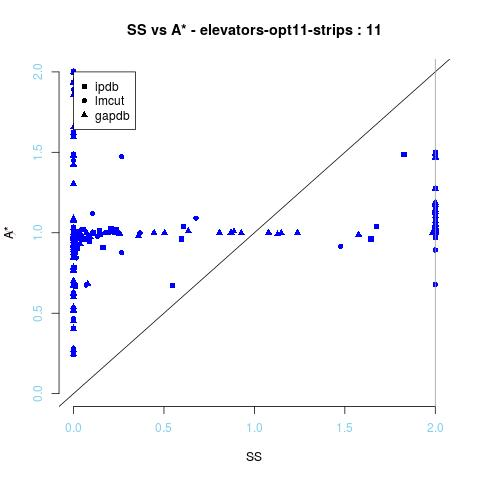
\includegraphics[width=\linewidth]{images/elevators-opt11-strips}
\endminipage\hfill
\minipage{0.32\textwidth}
  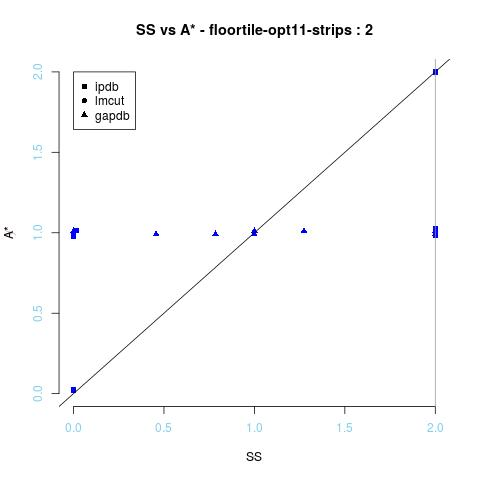
\includegraphics[width=\linewidth]{images/floortile-opt11-strips}
\endminipage\hfill
\minipage{0.32\textwidth}%
  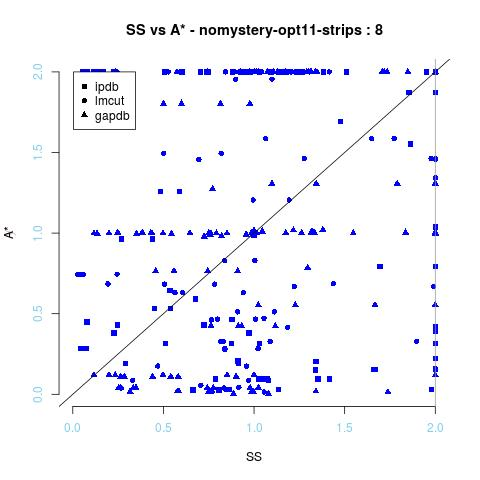
\includegraphics[width=\linewidth]{images/nomystery-opt11-strips}
\endminipage

%jump
\minipage{0.32\textwidth}
  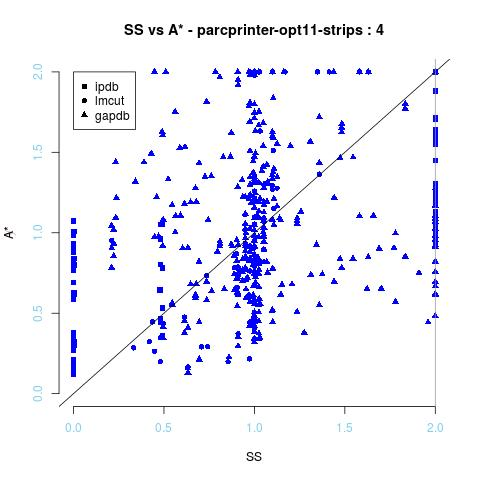
\includegraphics[width=\linewidth]{images/parcprinter-opt11-strips}
\endminipage\hfill
\minipage{0.32\textwidth}
  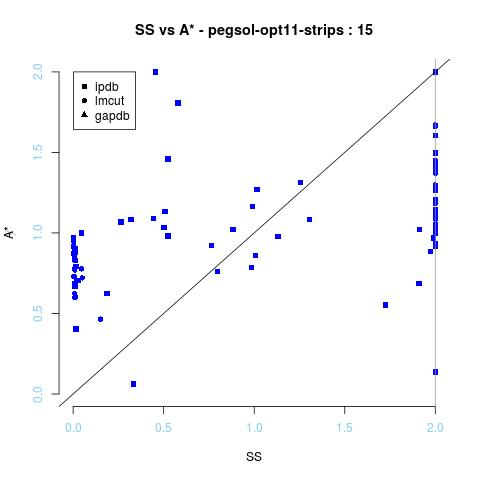
\includegraphics[width=\linewidth]{images/pegsol-opt11-strips}
\endminipage\hfill
\minipage{0.32\textwidth}
  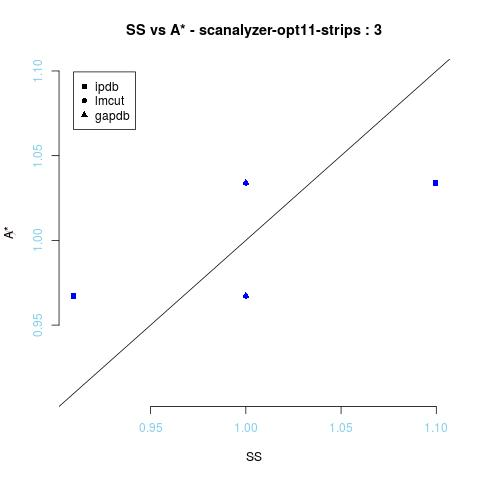
\includegraphics[width=\linewidth]{images/scanalyzer-opt11-strips}
\endminipage\hfill

%jump
\minipage{0.32\textwidth}
  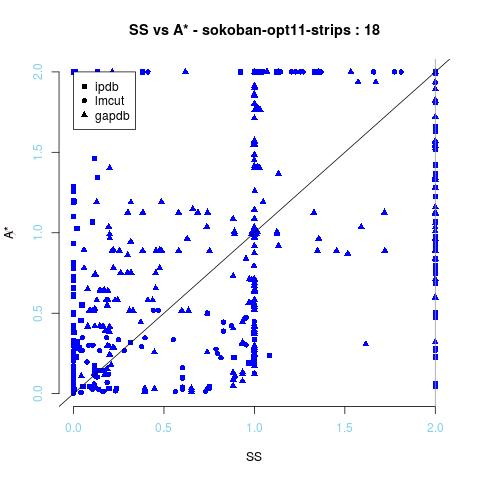
\includegraphics[width=\linewidth]{images/sokoban-opt11-strips}
\endminipage\hfill
\minipage{0.32\textwidth}
  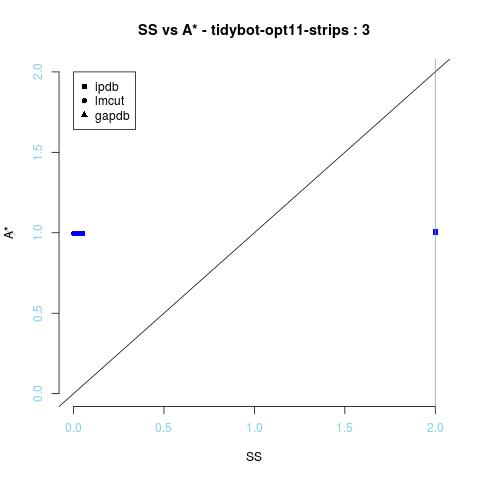
\includegraphics[width=\linewidth]{images/tidybot-opt11-strips}
\endminipage\hfill
\minipage{0.32\textwidth}
  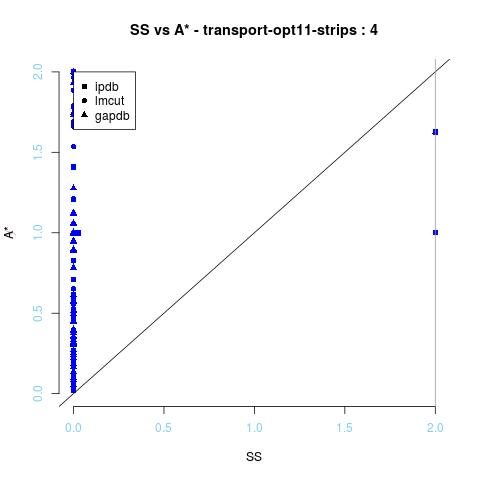
\includegraphics[width=\linewidth]{images/transport-opt11-strips} 
\endminipage\hfill

%jump
\minipage{0.32\textwidth}
  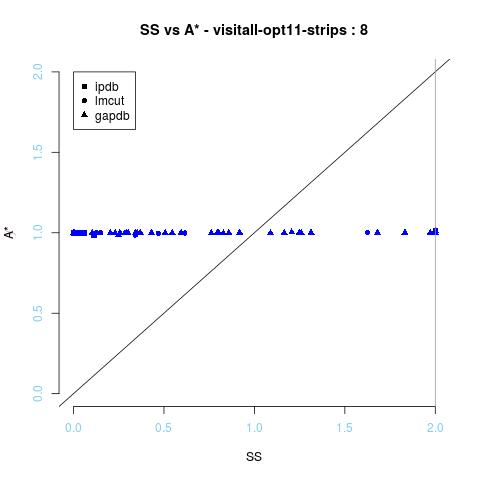
\includegraphics[width=\linewidth]{images/visitall-opt11-strips}
\endminipage\hfill
\minipage{0.32\textwidth}
  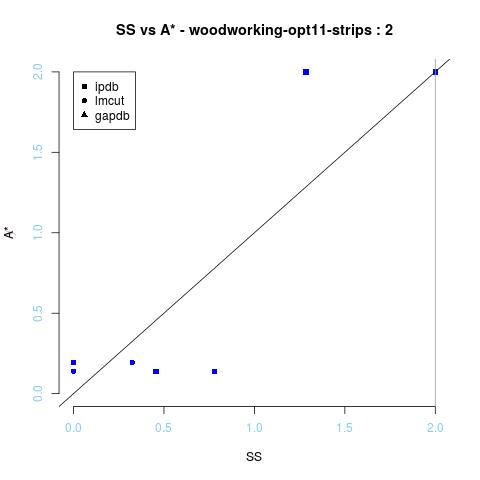
\includegraphics[width=\linewidth]{images/woodworking-opt11-strips}
\endminipage\hfill
\caption{\texttt{SS} vs A$\sp{*}$ ratios for the optimal domains $-$ The number of instances used in each domain are showed next to the name of the Domain.}\label{fig:img_analysis_domains}
\end{figure}
\newpage
\fi

\begin{table}[htb]
\centering
\begin{tabular}{lc}
\hline
Domain      & II and III ($\%$) \\ \hline
Elevators   & 78.57    \\
Floortile   & 96.08    \\
Nomystery   & 71.82    \\
Parcprinter & 70.50    \\
Pegsol      & 96.83    \\
Scanalyzer  & 100.00   \\
Sokoban     & 89.31    \\
Tidybot     & 100.00   \\
Transport   & 51.78    \\
Visitall    & 98.05    \\
Woodworking & 100.00   \\ \hline
\end{tabular}
\caption{Percentage of choices \texttt{SS} made correctly.}
\label{tb:per_ss_made_correctly}
\end{table}

In Table \ref{tb:per_ss_made_correctly} we present a single number for each domain representing the percentage of choices \texttt{SS} make correctly. From all the domains all are above of the 50$\%$ which means that at least the half of the points represent good relation of heuristics. With this experiment we prove that \texttt{SS} is not as bad as we thought it would be when we want to make selection.

\section{Explanation of the Experiments}
In order to verify the practical effectiveness of \texttt{GHS} we have implemented the algorithm in Fast Downward (Helmert, \citeyear{helmert2006fast}) and tested the A$\sp{*}$ performance using subsets of heuristics selected by \texttt{GHS} while minimizing different objective funcions.

We run two sets of experiments. In the first set we verify whether the approximations $\hat{J}$ and $\hat{T}$ provided by \texttt{CS} and \texttt{SS} allow \texttt{GHS} selects good subset selections for A$\sp{*}$ search tree size and running time. In the second set of experiments we test the effectiveness of \texttt{GHS} by measuring the total number of problem instances solved by A$\sp{*}$ using a heuristic subset selected by \texttt{GHS}.

\iffalse
In all our experiments we use a type system that assigned the same type for a node with the same $f-$value. Such a type system has shown to be effective in guiding \texttt{SS} to produce accurate tree size predictions in other application domains Lelis et al., (\citeyear{lelis2013predicting}), Lelis et al., (\citeyear{lelis2014memory}).
\fi

We ran our experiments on the 2011 International Planning Competition (\texttt{IPC}) instances. We used the 2011 instances instead of the 2014 instances because the former do not have problems with conditional effects, which are currently not handled by \texttt{PDB} heuristics. All experiments are run on $2.67$ GHz machines with 4GB, and are limited to 1,800 seconds of running time.

% ---
\section{Empirical Evaluation of $\hat{J}$ and $\hat{T}$}
\noindent
% ---
We test whether the approximation $\hat{J}$ provided by \texttt{CS} and \texttt{SS} allows \texttt{GHS} to make good subset selections. This test is made by comparing $J(\zeta\sp{'})$ with $J(\zeta)$, which is minimal. In contrast with objective function $J$, there is no easy way to find the minimum of $T$ for a subset in general. 

\iffalse
We experiment then with the special case in which all heuristics in $\zeta$ have the same evaluation time. This way we are able to test whether the estimates $\hat{T}$ are allowing \texttt{GHS} to make good subset selections while minimizing the A$\sp{*}$ running time. This is because by only selecting heuristics which have the same evaluation time, if \texttt{GHS} is making good subset selections with respect to $J$, then \texttt{GHS}, also must be making good subset selections with respect to $T$.
\fi

We collect values of $J(\zeta)$ and $J(\zeta\sp{'})$ as follows. For each problem instance $\nabla$ in our test set we generate a set of \texttt{PDB} heuristics using the \texttt{GA-PDB} algorithm (Edelkamp, \citeyear{edelkamp2007automated}) as described by Barley et al., (\citeyear{BarleySantiagoOver}) $-$ we call each \texttt{PDB} generated by this method a \texttt{GA-PDB}. The number of \texttt{GA-PDBs} generated is limited in this experiment by 1,200 seconds and 1GB of memory. Also, all \texttt{GA-PDBs} we generate have 2 millions entries each. The \texttt{GA-PDBs} generated form our $\zeta$ set. \texttt{GHS} then selects a subset $\zeta\sp{'}$ of $\zeta$. Finally, we use $h_{max}(\zeta\sp{'})$ and $h_{max}(\zeta)$ to independently try to solve $\nabla$. We call the system which uses A$\sp{*}$ with $h_{max}(\zeta)$ the \texttt{Max} approach. For \texttt{GHS} we allow 600 seconds for selecting $\zeta\sp{'}$ and for running A$\sp{*}$ with $h_{max}(\zeta\sp{'})$, and for \texttt{Max} we allow 600 seconds for running A$\sp{*}$ with $h_{max}(\zeta)$. Since we used 1,200 seconds to generate the heuristics, both \texttt{Max} and \texttt{GHS} were allowed 1,800 seconds in total for solving each problem. In this experiment we test both \texttt{CS} and \texttt{SS}.

% Please add the following required packages to your document preamble:
% \usepackage{multirow}
\begin{table}[]
\centering
\caption{Ratios of the number of nodes generated using $h_{max}(\zeta\sp{'})$ to the number of nodes generated using $h_{max}(\zeta)$}
\begin{tabular}{lrrrrrr}
\hline
\multirow{2}{*}{Domain} & \multicolumn{2}{c}{\texttt{SS}} & \multicolumn{2}{c}{\texttt{CS}}   & \multirow{2}{*}{|$\zeta$|} & \multirow{2}{*}{n} \\ \cline{2-5}
                        & Ratio    & |$\zeta\sp{'}$|   & Ratio  & |$\zeta\sp{'}$| &                            &                    \\ \hline
Barman                  & 1.11     & 17.70       & 1.50   & 30.25           & 5168.50                    & 20                 \\
Elevators               & 11.50     & 2.00       & 1.03   & 21.00           & 168.00                     & 1                  \\
Floortile               & 1.02     & 43.07       & 1.01   & 42.35           & 151.28                     & 14                 \\
Openstacks              & 1.00     & 1.00        & 1.00   & 1.00            & 390.69                     & 13                 \\
Parking                 & 1.00     & 5.52        & 1.01   & 7.26            & 21.73                      & 19                 \\
Pegsol                  & 1.00     & 31.00       & 1.00   & 57.00           & 90.00                      & 2                  \\
Scanalyzer              & 1.22     & 30.57       & 1.56   & 19.42           & 72.85                      & 7                  \\
Tidybot                 & 1.00     & 2.35        & 1.00   & 8.58            & 3400.17                    & 17                 \\
Transport               & 1.00     & 14.70        & 1.02   & 14.30           & 171.7                     & 10                  \\
Visitall                & 1.02     & 99.33       & 1.18   & 48.66           & 256.33                     & 3                  \\
Woodworking             & 32.42     & 3.00       & 199.65 & 5.00           & 1289.00                     & 5                  \\ \hline
\end{tabular}
\label{tb_one}
\end{table}


In this experiment we refer to the approach that runs A$\sp{*}$ guided by a heuristic subset selected by \texttt{GHS} using \texttt{CS} as \texttt{GHS+CS}. Similarly, we write \texttt{GHS+SS} when \texttt{SS} is used as predictor to make the heuristic subset selection.

Table \ref{tb_one} shows the average ratios of $J(\zeta\sp{'})$ to $J(\zeta)$ for both \texttt{SS} and \texttt{CS} in different problem domains. The value of $J$, for a given problem instance, is computed as the number of nodes expanded up to the largest $f$-layer which is fully expanded by all approaches tested (\texttt{Max, GHS} using \texttt{SS} and \texttt{GHS} using \texttt{CS}). We only present results for instances that are not solved during \texttt{GHS}'s \texttt{CS} sampling process. The column ``$n$'' shows the number of instances used to compute the averages of each row. We also show the average number of \texttt{GA-PDBs} generated (|$\zeta$|) and the average number of \texttt{GA-PDBs} selected by \texttt{GHS} (|$\zeta\sp{'}$|). This experiment shows that for most of the problems \texttt{GHS}, using \texttt{CS} or \texttt{SS}, is selecting good subset of $\zeta$ for A$\sp{*}$ search tree size and running time. For example, in Tidybot \texttt{GHS} selects only a few \texttt{GA-PDBs} out of thousands when using either \texttt{SS} or \texttt{CS}.

The exceptions in Table \ref{tb_one} are the ratios for Elevators, Scanalyzer and Woodworking. In Elevators \texttt{SS} has an average ratio of $11.50$ and \texttt{CS} of $1.03$. By looking at the ratios of \texttt{SS} for individual instances of Scanalyzer (results now show in Table \ref{tb_one}), we noticed that \texttt{SS} is able to make good selections for all but 3 of the 7 instances considered in this experiment. Since we do not know a priori what is the instance's optimal solution cost, \texttt{SS} samples nodes with $f$-values much larger than the instance's optimal solution cost.

\begin{table}[]
\centering
\caption{Coverage of \texttt{SS}, \texttt{CS} and \texttt{Max} on the 2011 IPC benchmarks. For GHS using only \texttt{GA-PDBs} heuristics.}
\label{my-label}
\begin{tabular}{lccc}
\hline
Domain      & SS & CS & Max \\ \hline
Barman      & 8          & 7          & 4           \\
Elevators   & 19         & 19         & 19          \\
Floortile   & 10         & 10         & 9           \\
Nomystery   & 20         & 20         & 20          \\
Openstacks  & 17         & 17         & 11          \\
Parcprinter & 17         & 15         & 14          \\
Parking     & 1          & 1          & 1           \\
Pegsol      & 19         & 19         & 19          \\
Scanalyzer  & 10         & 10         & 10          \\
Sokoban     & 20         & 20         & 20          \\
Tidybot     & 14         & 13         & 11          \\
Transport   & 14         & 14         & 14          \\
Visitall    & 18         & 18         & 18          \\
Woodworking & 12         & 11         & 12          \\ \hline
Total       & 199        & 194        & 182         \\ \hline
\end{tabular}
\label{tb_onlygapdbs}
\end{table}

The \texttt{SS}'s ability of sampling deep into the search space is not always harmful. For example, \texttt{SS} allows \texttt{GHS} to make good selections for instances of the Woodworking domain. By contrast, \texttt{CS}'s systematic approach to sampling only allow a shallow sample of the A$\sp{*}$ search tree. As a result, \texttt{GHS} makes a limited selection of heuristics to guide A$\sp{*}$ search. While \texttt{GHS} using \texttt{SS} selects an average of 3 heuristics in Woodworking instances, \texttt{GHS} using \texttt{CS} selects only an average of 5 heuristics. This difference on sampling strategies reflects on the number of problems solved by A$\sp{*}$. While \texttt{GHS+SS} solves 12 instances of the Woodworking domain, \texttt{GHS+CS} solves only 11. In total, out of the 280 instances of the \texttt{IPC} 2011 benchmark set, \texttt{GHS+SS} solves 199 problem instances in this experiment, while \texttt{GHS+CS} only solves 194 problem instances. (The numbers of instances solved are shown in Table \ref{tb_onlygapdbs}).

\section{Comparison with Other Planning Systems}
\noindent
The objective of this second set of experiments is to test the quality of the subset of heuristics \texttt{GHS} selects while optimizing different objective functions. Our evaluation metric is coverage, i.e., number of problems solved within a 1,800 second time limit. We note that the 1,800-second limit includes the time to generate $\zeta$, select $\zeta\sp{'}$, and run A$\sp{*}$ using $h_{max}(\zeta\sp{'})$. The $\zeta$ set of heuristics is composed of a number of different \texttt{GA-PDBs}, a \texttt{PDB} heuristic produced by the \texttt{iPDB} method Haslum et al., (\citeyear{haslum2007domain}) and the \texttt{LM-Cut} heuristic (Pommerening and Helmert, \citeyear{PommereningH13}). The generation of \texttt{GA-PDBs} is limited by 600 seconds and 1GB of memory. We use one fourth of 600 seconds to genetate \texttt{GA-PDBs} with each of the following number of entries: $\{2 \cdot 10\sp{3}, 2 \cdot 10\sp{4}, 2 \cdot 10\sp{5}, 2 \cdot 10\sp{6}\}$. Our approach allows one to generate up to thousands of \texttt{GA-PDBs}. For every problem instance, we use exactly the same $\zeta$ set for \texttt{Max} and all \texttt{GHS} approaches.

\section{Systems Tested}
\noindent
\texttt{GHS} is tested while minimizing the A$\sp{*}$ search tree size (\texttt{Size}) and the A$\sp{*}$ running time (\texttt{Time}). We also use \texttt{GHS} to maximize the sum of heuristic values in the state space (\texttt{Sum}), as suggested by Rayner et al., (\citeyear{raynersss13}). Rayner et al., (\citeyear{raynersss13}) assumed that one could uniformly sample states in the state space in order to estimte the sum of the heuristic values for a given heuristic subset. Since we are not aware of any method to uniformly sample the state space of domain-independent problems, we adapted the Rayner et al., (\citeyear{raynersss13})'s method by using \texttt{SS} to estimate the sum of heuristic values in the search tree rooted at $\nabla$'s start state. We write \texttt{Size+SS} to refer to the approach that used A$\sp{*}$ guided by a heuristic selected by \texttt{GHS} while minimizing an estimate of the search tree size provided by \texttt{SS}. We follow the same pattern to name the other possible combinations of objective functions and prediction algorithms (e.g., \texttt{Time}+\texttt{CS}).

In addition to experimenting with all combinations of prediction algorithms (\texttt{CS} and \texttt{SS}) and objective functions (\texttt{Time}, \texttt{Size}), we also experiment with an approach that minimizes both the search tree size and the running time as follows. First we create a pool of heuristics $\zeta$ composed solely of \texttt{GA-PDB} heuristics, then we apply \texttt{GHS} while minimizing tree size and using \texttt{SS} as predictor. We call the selection of a subset of \texttt{GA-PDBs} as the \textit{first selection}. Once the first selection is made, we test all possible combinations of the resulting $h_{max}(\zeta\sp{'})$ added to \texttt{iPDB} and \texttt{LM-Cut} heuristics while minimizing the running time as estimated by \texttt{CS}$-$we call this step the \textit{second selection}. We call the overall approach \texttt{Hybrid}.
%As explained above, in this setting \texttt{GHS} minimizes $J$ and $T$ simultaneaously, as all heuristics in $\zeta$ have the same evaluation time (Theorem \ref{th:theorem_evaluation_time_heuristic})

The intuition behind \texttt{Hibrid} is that we apply \texttt{GHS} with its strongest settings. \texttt{GHS} makes good selections respect to $J$ and $T$ when selecting from a pool of heuristics with the same evaluation time. After such a selection is made, we reduce the size of the pool of heuristics from possible thousands to only three (the maximum of a subset of the initial \texttt{GA-PDBs, iPDB}, and \texttt{LM-Cut}). With only three heuristics we are able to choose the exact combination that minimizes the A$\sp{*}$ running time the most. The reason we chose to use \texttt{SS} instead of \texttt{CS} for the first selection in \texttt{Hybrid} is that the former is able to make better subset selections in this setting, as suggested by the results discussed in the previous Chapter \ref{ch:rghs}. Finally, as we show below, \texttt{CS} is more effective if one is interested in minimizing the A$\sp{*}$ running time while selecting from a pool of heuristic with different evaluation times. That is why we use \texttt{CS} as predictor for the second selection in \texttt{Hybrid}.

We compare the coverage of the \texttt{GHS} approaches with several other state-of-the-art planners. Namely, we experiment with RIDA$\sp{*}$ Barley et al., (\citeyear{BarleySantiagoOver}), two variants of StoneSoup (StSp1 and StSp2) as described by Nissim et al., (\citeyear{nissim2011computing}), two versions of Symba (SY1 and SY2) (Torralba, \citeyear{torralba2015phd}), and A$\sp{*}$ being independently guided by the maximum of all heuristics in $\zeta$ (\texttt{Max}), \texttt{iPDB}, \texttt{LM-cut} and \texttt{Merge $\&$ Shrink} (\texttt{M$\&$S}) Nissim et al., (\citeyear{nissim2011computing}). The results are presented in Table \ref{tb_two}.

\section{Discussion of the Results}
\noindent
The system that solves the largest number of instances is \texttt{Hybrid}---it solves 219 problems on average. As explained above, we combine in \texttt{Hybrid} the strengths of both \texttt{SS} and \texttt{CS} in a single system. \texttt{GHS} uses \texttt{SS} to select heuristics from a pool of heuristics with similar evaluation time, and only then \texttt{CS} is used for selecting heuristics with different evaluation times. This strategy has proven particularly effective on the Barman domain where \texttt{Hybrid}'s first selection is able to select good subsets of \texttt{GA-PDBs} and its second selection is able to recognize that it must not include the \texttt{iPDB} and \texttt{LM-Cut} heuristics to the subset selected by its first selection. As a result, \texttt{Hybrid} solves more problems on this domain than any other \texttt{GHS} approach.

\texttt{Time}+\texttt{CS} also performed well in our experiments$-$the approach solves 214 problems on average. Clearly \texttt{Hybrid} and \texttt{Time}+\texttt{CS} are far superior to all other approaches tested. For example, \texttt{Size}+\texttt{SS} and \texttt{Sum} solves only 204 and 207 problems, respectively. While minimizing the search tree size or maximizing the sum of heuristic values, \texttt{GHS} will tend to add accurate heuristics to the selected subset, independently of their evaluation time. As a result, if not minimizing the running time, \texttt{GHS} often adds the \texttt{LM-Cut} heuristic to $\zeta\sp{'}$ as \texttt{LM-Cut} is often the heuristic that is able to reduce the most the search tree size and to increase the most the sum of heuristic values. However, \texttt{LM-Cut} is very computationally expensive, and in various cases the search is faster if \texttt{LM-Cut} is not in $\zeta\sp{'}$. Both \texttt{Hybrid} and \texttt{Time}+\texttt{CS} are able to recognize when \texttt{LM-Cut} should not be included in $\zeta\sp{'}$ because they account for the heuristics' evaluation time.

% Please add the following required packages to your document preamble:
% \usepackage{multirow}
\begin{table}[htb]
\footnotesize\setlength{\tabcolsep}{1.8pt}
\centering
\caption{Coverage of different planning systems on the 2011 \texttt{IPC} benchmarks. For the \texttt{GHS} and \texttt{Max} approaches we also present the average number of heuristics \texttt{GHS} selects (|$\zeta\sp{'}$|).}
\begin{tabular}{lrrrrrrrrrrrrrrr}
\hline
\multirow{2}{*}{Domains} & 
\multirow{2}{*}{\texttt{Hybrid}} & 
\multicolumn{2}{c}{\texttt{CS}} & 
\multicolumn{2}{c}{\texttt{SS}} & 
\multirow{2}{*}{\texttt{Sum}} & 
\multirow{2}{*}{\texttt{Max}} &
\multirow{2}{*}{RIDA$\sp{*}$} & 
\multirow{2}{*}{SY1} & 
\multirow{2}{*}{SY2} & 
\multirow{2}{*}{StSp1} & 
\multirow{2}{*}{StSp2} & 
\multirow{2}{*}{iPDB} & 
\multirow{2}{*}{LM-Cut} & 
\multirow{2}{*}{M$\&$S} \\ \cline{3-6}
                         &                                    & \texttt{Time} & \texttt{Size} & \texttt{Time} & \texttt{Size} &                                 &                       &                      &                      &                        &                        &                                 &                       &                         &                         \\ \hline
Barman&         7&      5&     4&    4&    4&    4&   4&    4&    10&  11&    4&    4&    4&     4&   4\\
Elevators&     19&     19&    19&   19&   19&   19&  19&   19&    20&  20&   18&   18&   18&    17&  12\\
Floortile&     15&     14&    14&   14&   14&   14&  14&   14&    14&  14&   14&   14&   14&     8&  10\\
Nomystery&     20&     20&    20&   19&   19&   20&  20&   20&    16&  16&   20&   20&   14&    19&  18\\
Openstacks&    17&     17&    15&   17&   15&   15&  11&   15&    20&  20&   17&   17&   15&    17&  17\\
Parcprinter&   18&     18&    18&   16&   15&   19&  18&   18&    17&  17&   18&   18&   17&    16&  16\\
Parking&        7&      7&     2&    7&    2&    2&   2&    7&     2&   1&    5&    5&    2&     7&   7\\
Pegsol&        18&     18&    19&   19&   19&   19&  19&   19&    19&  20&   19&   19&   17&    20&  19\\
Scanalyzer&    13&     14&    12&   11&   14&   14&  14&   14&     9&   9&   14&   14&   12&    10&  11\\
Sokoban&       20&     20&    20&   20&   20&   20&  20&   20&    20&  20&   20&   20&   20&    20&  20\\
Tidybot&       17&     16&    16&   16&   16&   16&  15&   17&    15&  17&   16&   16&   16&    14&   9\\
Transport&     14&     13&    10&   11&   13&   11&   9&   10&    10&  11&    7&    8&    6&     8&   7\\
Visitall&      18&     18&    18&   15&   18&   18&  18&   18&    12&  12&   16&   16&   10&    16&  16\\
Woodworking&   16&     15&    15&   12&   16&   16&  16&   15&    20&  20&   15&   15&   15&     9&   9\\ \hline
Total&        219&    214&   202&  200&  204&  207& 199&  210&   204& 208&  203&  204&  180&   185& 175\\ \hline
\end{tabular}
\label{tb_two}
\end{table}

Note that the difference on the number of problems solved by \texttt{Time}+\texttt{CS} and \texttt{Time}+\texttt{SS}: While the former solves 214 instances, the latter solved only 200. We conjecture that this happens because \texttt{SS} is not able to detect duplicated nodes during sampling. As a result, \texttt{SS} often overestimates by several orders of magnitude the actual A$\sp{*}$'s running time. Similarly to the \texttt{Size} and \texttt{Sum} approaches, due to \texttt{SS}'s overestimations, \texttt{Time}+\texttt{SS} often mistakenly adds the accurate but expensive \texttt{LM-Cut} heuristic in cases where the A$\sp{*}$ search would be faster without \texttt{LM-Cut}'s guidence. 
\iffalse
For example, although \texttt{iPDB} tends to prune fewer nodes than \texttt{LM-Cut} in Woodworking instances, \texttt{iPDB} is the heuristic of choice in that domain. This is because its evaluation time is much smaller than \texttt{LM-Cut}'s. \texttt{Time}+\texttt{CS} solves 7 Parking instances on average as it correctly selects \texttt{iPDB} and leaves \texttt{LM-Cut} out of $\zeta\sp{'}$. By contrast, likely due to its prediction overestimation, \texttt{Time}+\texttt{SS} solves 7 parking instances because wrongly estimates \texttt{LM-Cut} that will reduce overall search time and adds the heuristic to its selected subset. Notice, that \texttt{Size+CS} and \texttt{Size+SS} also do poorly Parking instances as they also always select \texttt{LM-Cut}.
\fi

RIDA$\sp{*}$ is the most similar system to \texttt{GHS}, as it also selects a subset of heuristics from a pool of heuristics by using an evaluation method similar to \texttt{CS}. RIDA$\sp{*}$ uses a systematic approach for selecting a subset of heuristics. Namely, it starts with an empty subset and evaluates all subsets of size $i$ before evaluating subsets of size $i+1$. This procedure allows RIDA$\sp{*}$ to consider only tens of heuristics in their pool. By contrast, \texttt{GHS} is able to consider thousands of heuristics while making its selection.

The ability to handle large set of heuristics can be helpful, even if most of the heuristics in the set are redundant with each other$-$as is the case with the \texttt{GA-PDBs}. The process of generating \texttt{GA-PDBs} is stochastic, thus one increases the chances of generating helpful heuristic by generating a large number of them. \texttt{GHS} is an effective method for selecting a small set of informative heuristics from a large set of mostly uninformative ones. This is illustrated in Table \ref{tb_two} on the Transport domain. Compared to systems which use multiple heuristics (StSp1 and 2, and RIDA$\sp{*}$), \texttt{Time}+\texttt{CS} solves the largest number of Transport instances, which is due to the selection of a few key \texttt{GA-PDBs}.

The best \texttt{GHS} approach, \texttt{Hybrid}, substantially outperforms the number of instances solved by \texttt{Max}; \texttt{Hybrid} solves on average more than 20 instances than \texttt{Max}. Finally, \texttt{Hybrid} and \texttt{Time}+\texttt{CS} substantially outperforms all other approaches tested, with RIDA$\sp{*}$ being the closest competitor with 210 instances solved.

\clearpage
% ---


% ---
%\section{Vestibulum ante ipsum primis in faucibus orci luctus et ultrices posuere cubilia Curae}
% ---

%\lipsum[21-22]

% ---
% segundo capitulo de Resultados
% ---
%\chapter{Nam sed tellus sit amet lectus urna ullamcorper tristique interdum
%elementum}
% ---

% ---
%\section{Pellentesque sit amet pede ac sem eleifend consectetuer}
% ---

%\lipsum[24]

% ----------------------------------------------------------
% Finaliza a parte no bookmark do PDF
% para que se inicie o bookmark na raiz
% e adiciona espaço de parte no Sumário
% ----------------------------------------------------------
\phantompart

% ---
% Conclusão
% ---
%\chapter{Conclusão}
% ---
% PARTE
% ----------------------------------------------------------
\part{Conclusion}
% ----------------------------------------------------------
%% abtex2-modelo-include-comandos.tex, v-1.9.5 laurocesar
%% Copyright 2012-2015 by abnTeX2 group at http://www.abntex.net.br/ 
%%
%% This work may be distributed and/or modified under the
%% conditions of the LaTeX Project Public License, either version 1.3
%% of this license or (at your option) any later version.
%% The latest version of this license is in
%%   http://www.latex-project.org/lppl.txt
%% and version 1.3 or later is part of all distributions of LaTeX
%% version 2005/12/01 or later.
%%
%% This work has the LPPL maintenance status `maintained'.
%% 
%% The Current Maintainer of this work is the abnTeX2 team, led
%% by Lauro César Araujo. Further information are available on 
%% http://www.abntex.net.br/
%%
%% This work consists of the files abntex2-modelo-include-comandos.tex
%% and abntex2-modelo-img-marca.pdf
%%

% ---
% Este capítulo, utilizado por diferentes exemplos do abnTeX2, ilustra o uso de
% comandos do abnTeX2 e de LaTeX.
% ---
 
\chapter{Concluding Remarks}\label{ch:conclusions}

\iffalse
\chapterprecis{The purpose of this section is to introduce the meta-reasoning proposed.}\index{sinopse de capítulo}
\fi

% ---
%\section{Conclusions}
% ---
\noindent
This dissertation showed that the problem of finding the optimal subset of a set of heuristics $\zeta$ for a given problem task is solved using the models of A$\sp{*}$ search tree size and, under mild assumptions, with respect to the A$\sp{*}$ running time. Thus, the \texttt{GHS} algorithm which selects heuristics from $\zeta$ one at a time is able to produce a subset $\zeta\sp{'}$ such that the number of nodes expanded by A$\sp{*}$ while guided by the heuristics $\zeta\sp{'}$ is 10\% optimal. Furthermore, if all heuristics in $\zeta$ have the same evaluation time, then we have the same good subset selection with respect to running time. In addition to minimizing the search tree size and the running time, we also experimented with an objective function that accounts for the sum of heuristic values in the state-space, as suggested by Rayner et al., (\citeyear{raynersss13}).

Since we cannot compute the values of the objective functions exactly, \texttt{GHS} effectiveness depends on the quality of the approximations we can obtain. We tested two prediction algorithms, \texttt{CS} and \texttt{SS}, for estimating the values of the objective functions and showed empirically that both \texttt{CS} and \texttt{SS} allow \texttt{GHS} to make near-optimal and good subset selections with respect to the search tree size and running time respectively.

Finally, experiments on optimal domain-independent problems showed that \texttt{GHS} minimizing approximations of the A$\sp{*}$ running time outperformed all the other approaches tested, which demostrates the effectiveness of our method for the heuristic subset selection problem.

\clearpage
% ---


%\lipsum[31-33]

% ----------------------------------------------------------
% ELEMENTOS PÓS-TEXTUAIS
% ----------------------------------------------------------
\postextual
% ----------------------------------------------------------

% ----------------------------------------------------------
% Referências bibliográficas
% ----------------------------------------------------------
\bibliography{abntex2-modelo-references}

% ----------------------------------------------------------
% Glossário
% ----------------------------------------------------------
%
% Consulte o manual da classe abntex2 para orientações sobre o glossário.
%
%\glossary

% ----------------------------------------------------------
% Apêndices
% ----------------------------------------------------------

\if false
% ---
% Inicia os apêndices
% ---
\begin{apendicesenv}

% Imprime uma página indicando o início dos apêndices
\partapendices

% ----------------------------------------------------------
\chapter{Quisque libero justo}
% ----------------------------------------------------------

\lipsum[50]

% ----------------------------------------------------------
\chapter{Nullam elementum urna vel imperdiet sodales elit ipsum pharetra ligula
ac pretium ante justo a nulla curabitur tristique arcu eu metus}
% ----------------------------------------------------------
\lipsum[55-57]

\end{apendicesenv}
% ---

\fi

% ----------------------------------------------------------
% Anexos
% ----------------------------------------------------------

\if false
% ---
% Inicia os anexos
% ---
\begin{anexosenv}

% Imprime uma página indicando o início dos anexos
\partanexos

% ---
\chapter{Morbi ultrices rutrum lorem.}
% ---
\lipsum[30]

% ---
\chapter{Cras non urna sed feugiat cum sociis natoque penatibus et magnis dis
parturient montes nascetur ridiculus mus}
% ---

\lipsum[31]

% ---
\chapter{Fusce facilisis lacinia dui}
% ---

\lipsum[32]

\end{anexosenv}

\fi
%---------------------------------------------------------------------
% INDICE REMISSIVO
%---------------------------------------------------------------------
\phantompart
\printindex
%---------------------------------------------------------------------

\end{document}